% ------------------------------------------------------------
% This latex template is based on the version created by Xiao Xiong (NTU).
% Compile main_QE_report.tex to generate the QE report.
%
% Author: Tan Zheng Hui Ernest, NTU, Singapore
% Date: 8 Apr 2020
% ------------------------------------------------------------


% \input{setting}     % Input Global settings
% 1. Define your report format here
\documentclass[12pt,a4paper,twoside]{report}

% 2. Specify the packages to be included
\usepackage{amssymb,amsmath,epsfig,fancyheadings,cite}

\oddsidemargin  +0.10in %
\evensidemargin +0.00in %
\topmargin      +0.15in %
\textheight     +8.50in %
\textwidth      +6.25in %

\pagestyle{plain}

\font\Bold=cmbx10 scaled \magstep3
\def\EndOfProof{\nolinebreak\ \hfill\rule{1.5mm}{2.7mm}}
\def\endOfProof{\ \hfill\rule{1.5mm}{2.7mm}}
\def\proof{\noindent \textbf{Proof:}\quad}

\newcounter{theorem}
\newtheorem{theorem}{Theorem}
\renewcommand{\thetheorem}{\thechapter.\arabic{theorem}}

\newcounter{lemma}
\newtheorem{lemma}{Lemma}
\renewcommand{\thelemma}{\thechapter.\arabic{lemma}}

\newcounter{corollary}
\newtheorem{corollary}{Corollary}
\renewcommand{\thecorollary}{\thechapter.\arabic{corollary}}

\newcounter{definition}
\newtheorem{definition}{Definition}
\renewcommand{\thedefinition}{\thechapter.\arabic{definition}}
\renewcommand{\bibname}{References}

% Define some new macros
%\def\addnotation #1: #2#3{$#1$\indent \parbox{5in}{#2 \dotfill  \pageref{#3}}}
\def\addnotation #1: #2#3{$#1$ & #2 & \pageref{#3}}
\def\newnot#1{\label{#1}}

\usepackage{amsmath}
\usepackage[cmintegrals]{newtxmath}
\usepackage{longtable}
\usepackage{graphicx}
\usepackage{subcaption}

\begin{document}    % Start of the text

% -------------------------------------------------------------------------------- %
% --------------------------- Part I. Front Matters ------------------------------ %
% -------------------------------------------------------------------------------- %

\title{\sc
\vspace{-0.5in} Find Better Trajectory for Diffusion Model Fast Sampling\\
\vspace*{0.3in} \centering
\resizebox*{0.5\textwidth}{!}{
\includegraphics{figure/NTU_new_logo.eps}}\\[1em]}

\author{
Qualifying Examination Report\\
Submitted to the School of Computer Science and Engineering\\
of the Nanyang Technological University\\[1em]
by\\[1em]
{\rm\bf Xu Shifeng}\\[1.5em]
for the Confirmation for Admission \\
to the Degree of Doctor of Philosophy\\[1.5em]
}

\date{\today}
\maketitle
\thispagestyle{empty}        % no page number on this front cover page
       % Input the Cover page

\setlength{\baselineskip}{20pt plus 1pt minus 1pt} % Use 1-1/2 spacing for whole document
\pagenumbering{roman}   % Use small roman digits for the page number of front matters

\chapter* {Abstract}
\addcontentsline{toc}{section}{\numberline{}\hspace{-0.35in}{\bf Abstract}}
% Add the Abstract to the table of contents using the specified format

Diffusion models are emerging generative models with promising performance. They inject noise into training data progressively in forward process, and then remove noise from perturbed data iteratively in reverse process. The reverse process is for sample generation and therefore is also called sampling process.
Typically, sampling process requires hundreds to thousands of steps, which is very slow and not applicable to time-sensitive scenario. Several prior works have made efforts to speed up the sampling process for efficiency. And in those efficiency-focused works, the main goal is to use fewer steps in sampling trajectory.
However, in most cases, fewer sampling steps are achieved at the expense of sampling quality. In this work, it proposes a practical post-hoc method to improve the sampling quality: given a predefined trajectory, it searches for a new trajectory with the same step count but generates better result.
During trajectory optimization, it focuses on the prediction error of diffusion model with a novel variance-reduction guidance (VRG). VRG reduces the impact of prediction error by optimizing the step size in sampling trajectory, and consequently improves the sampling quality.
VRG is model-agnostic and training-free. It is suitable for continuous-time and discrete-time sampling process, and also applicable to conditional and unconditional generation. Experiments are conducted on state-of-the-art works, and the result comparison demonstrates that VRG can improve sampling quality significantly.
    % Input the abstract and acknowledgement
\chapter* {Acknowledgments}
\addcontentsline{toc}{section}{\numberline{}\hspace{-.35in}{\bf
Acknowledgments}}

I would like to express my sincere thanks and appreciation to my supervisor, A/P Adams Wai Kin Kong, for his guidance and patience in imparting valuable knowledge to me. I would also like to extend my thanks to RSS fund for the support and stipend of my Ph.D program. 
Last, but not least, I want to thank my family for their strong support and encouragement as I undertake this Ph.D career.



\setcounter{secnumdepth}{3} % section numbering depth
\setcounter{tocdepth}{4}    % count to the depth of sections
\tableofcontents            % table of contents appears here

\newpage
\addcontentsline{toc}{section}{\numberline{}\hspace{-.35in}{\bf List of Figures}}
\listoffigures              % list of figures appears here

\newpage
\addcontentsline{toc}{section}{\numberline{}\hspace{-.35in}{\bf List of Tables}}
\listoftables              % list of tables appears here

% \newpage
% \addcontentsline{toc}{section}{\numberline{}\hspace{-.35in}{\bf List of Abbreviations}}
% \chapter* {List of Abbreviations}
%\addcontentsline{toc}{section}{\numberline{}\hspace{-.35in}{\bf List
%of Abbreviations}}

\begin{longtable}{ll}		
A/A	& Air-to-Air\\
A/G	& Air-to-Ground \\
ACARS	& Aircraft Communications Addressing and Reporting System \\
ACS	& Aeronautical Communication System\\
ADS-B	& Automatic Dependent Surveillance - Broadcast\\
AeroMACS	& Aeronautical Mobile Airport Communications System\\
AMACS	& All-purpose Multichannel Aviation Communication System \\
APNT	& Alternative Positioning, Navigation and Timing\\
AS	& Air-Station\\
ATM	& Air Traffic Management\\
AWGN	& Additive White Gaussian Noise\\
B-AMC	& Broadband-Aeronautical Mobile Communications\\
BER	& Bit Error Rate\\
BICM	& Bit Interleaved Coded Modulation\\
CDF	& Cumulative Distribution Function\\
CDM	& Code Domain Multiplexing\\
CDMA	& Code Division Multiple Access\\
CR	& Cognitive Radio\\
CSI	& Channel State Information\\
D2D	& Device-to-Device\\
D8PSK	& Differential 8 Phase Shift Keying\\
DME	& Distance Measurement Equipment \\
DMT	& Diversity-Multiplexing Tradeoff\\
EUROCONTROL	& European Organization for the Safety of Air Navigation\\
FAA	& Federal Aviation Administration\\
FCI	& Future Communications Infrastructure\\
FD	& Full-Duplex\\
FDD	& Frequency Division Duplex\\
FDMA	& Frequency Division Multiple Access\\
G/A	& Ground-to-Air\\
GPS	& Global Positioning System\\
GS	& Ground Station\\
GSM	& Global Systems for Mobile\\
HBD	& Hybrid-Duplex\\
HD	& Half-Duplex\\
HF	& High Frequency\\
IBFD	& In-Band Full Duplex\\
II	& Interference Ignorant\\
JD	& Joint Detection\\
LDACS	& L-band Digital Aeronautical Communication System\\
LDS	& Low Density Signature\\
LO	& Local Oscillator\\
LOS	& Line-of-Sight\\
LTE	& Long Term Evolution\\
MGR	& Multiplexing Gain Region\\
MIMO	& Multiple-Input Multiple-Output\\
MPA	& Message Passing Algorithm\\
MUSA	& Multi User Shared Access\\
NLOS	& Non Line-of-Sight\\
NOMA	& Non-Orthogonal Multiple Access\\
OMA	& Orthogonal Multiple Access\\
PDF	& Probability Density Function\\
PDM	& Power Domain Multiplexing\\
PU	& Primary User\\
QoS	& Quality-of-Service\\
QS-PQPSK	& Quad State-Paired QPSK\\
RHS	& Right Hand Side\\
RSSI	& Received Signal Strength Indicator\\
RV	& Random Variable\\
SCMA	& Sparse Code Multiple Access\\
SESAR	& Single European Sky ATM Research\\
SI	& Self Interference\\
SIC	& Successive Interference Cancellation\\
SNR	& Signal-to-Noise Ratio\\
SOI	& Signal-of-Interest\\
SSD	& Signal Space Diversity\\
SSR	& Secondary Surveillance Radar \\
STBC QS-PQPSK	& Space-Time Block Coded QS-PQPSK\\
SU	& Secondary User\\
TACAN	& Tactical Air Navigation \\
TDD	& Time Division Duplex\\
TDMA	& Time Division Multiple Access\\
UAT	& Universal Access Transceiver \\
UAV	& Unmanned Aerial Vehicle\\
UMTS & Universal Mobile Telecommunications System\\
VDL	& VHF Data Link\\
VDL-2	& VDL-Mode 2\\
VDL-3	& VDL-Mode 3\\
VDL-4	& VDL-Mode 4\\
VHF	& Very High Frequency\\
\end{longtable}


%\begin{tabular}{p{100pt}l}
  %% after \\: \hline or \cline{col1-col2} \cline{col3-col4} ...
		%
%A/A	& Air-to-Air\\
%A/G	& Air-to-Ground \\
%ACARS	& Aircraft Communications Addressing and Reporting System \\
%ACS	& Aeronautical Communication System\\
%ADS-B	& Automatic Dependent Surveillance - Broadcast\\
%AeroMACS	& Aeronautical Mobile Airport Communications System\\
%AMACS	& All-purpose Multichannel Aviation Communication System \\
%APNT	& Alternative Positioning, Navigation and Timing\\
%AS	& Air-Station\\
%ATM	& Air Traffic Management\\
%AWGN	& Additive White Gaussian Noise\\
%B-AMC	& Broadband-Aeronautical Mobile Communications\\
%BER	& Bit Error Rate\\
%BICM	& Bit Interleaved Coded Modulation\\
%CDF	& Cumulative Distribution Function\\
%CDM	& Code Domain Multiplexing\\
%CDMA	& Code Division Multiple Access\\
%CR	& Cognitive Radio\\
%CSI	& Channel State Information\\
%D2D	& Device-to-Device\\
%D8PSK	& Differential 8 Phase Shift Keying\\
%DME	& Distance Measurement Equipment \\
%DMT	& Diversity-Multiplexing Tradeoff\\
%EUROCONTROL	& European Organization for the Safety of Air Navigation\\
%FAA	& Federal Aviation Administration\\
%FCI	& Future Communications Infrastructure\\
%FD	& Full-Duplex\\
%FDD	& Frequency Division Duplex\\
%FDMA	& Frequency Division Multiple Access\\
%G/A	& Ground-to-Air\\
%GPS	& Global Positioning System\\
%GS	& Ground Station\\
%GSM	& Global Systems for Mobile\\
%HBD	& Hybrid-Duplex\\
%HD	& Half-Duplex\\
%HF	& High Frequency\\
%IBFD	& In-Band Full Duplex\\
%II	& Interference Ignorant\\
%JD	& Joint Detection\\
%LDACS	& L-band Digital Aeronautical Communication System\\
%LDS	& Low Density Signature\\
%LO	& Local Oscillator\\
%LOS	& Line-of-Sight\\
%LTE	& Long Term Evolution\\
%MGR	& Multiplexing Gain Region\\
%MIMO	& Multiple-Input Multiple-Output\\
%MPA	& Message Passing Algorithm\\
%MUSA	& Multi User Shared Access\\
%NLOS	& Non Line-of-Sight\\
%NOMA	& Non-Orthogonal Multiple Access\\
%OMA	& Orthogonal Multiple Access\\
%PDF	& Probability Density Function\\
%PDM	& Power Domain Multiplexing\\
%PU	& Primary User\\
%QoS	& Quality-of-Service\\
%QS-PQPSK	& Quad State-Paired QPSK\\
%RHS	& Right Hand Side\\
%RSSI	& Received Signal Strength Indicator\\
%RV	& Random Variable\\
%SCMA	& Sparse Code Multiple Access\\
%SESAR	& Single European Sky ATM Research\\
%SI	& Self Interference\\
%SIC	& Successive Interference Cancellation\\
%SNR	& Signal-to-Noise Ratio\\
%SOI	& Signal-of-Interest\\
%SSD	& Signal Space Diversity\\
%SSR	& Secondary Surveillance Radar \\
%STBC QS-PQPSK	& Space-Time Block Coded QS-PQPSK\\
%SU	& Secondary User\\
%TACAN	& Tactical Air Navigation \\
%TDD	& Time Division Duplex\\
%TDMA	& Time Division Multiple Access\\
%UAT	& Universal Access Transceiver \\
%UAV	& Unmanned Aerial Vehicle\\
%UMTS & Universal Mobile Telecommunications System\\
%VDL	& VHF Data Link\\
%VDL-2	& VDL-Mode 2\\
%VDL-3	& VDL-Mode 3\\
%VDL-4	& VDL-Mode 4\\
%VHF	& Very High Frequency\\
%
%\end{tabular}
      % Input the list of abbreviations and notations

% \newpage
% \addcontentsline{toc}{section}{\numberline{}\hspace{-.35in}{\bf List of Publications}}
% \chapter* {List of Publications}
%\addcontentsline{toc}{chapter}{\numberline{}\hspace{-0.24in}{\bf
%Publication}}

\section* {International Conferences}
\begin{itemize}
    \item Tan Zheng Hui Ernest, Anoop Kumar Krishna, AS Madhukumar, and Rajendra Prasad Sirigina ``On the efficiency improvements to aeronautical waveforms and integrated modular avionics systems'', Proc IEEE/AIAA 35th Digit. Avionics Syst. Conf. (DASC), 2016. IEEE,
2016, pp. 1–8.
		\item Tan Zheng Hui Ernest, Rajendra Prasad Sirigina, AS Madhukumar, and Anoop Kumar Krishna ``On the Performance Analysis of Hybrid-Duplex Systems for Aeronautical Communications'', IEEE 87th Veh. Technol. Conf., 2018, Accepted.
\end{itemize}

\section* {International Journals}
\begin{itemize}
    \item Tan Zheng Hui Ernest, AS Madhukumar, Rajendra Prasad Sirigina, and Anoop Kumar Krishna ``On the Outage Analysis and Finite SNR
Diversity-Multiplexing Tradeoff of Hybrid-Duplex Systems for Aeronautical Communications'', Under review at IEEE Trans. Wireless Commun.
		\item Tan Zheng Hui Ernest, AS Madhukumar, Rajendra Prasad Sirigina, and Anoop Kumar Krishna ``A Hybrid-Duplex System with Joint Detection
for Interference-Limited UAV Communications'', Under review at IEEE Journ. Selected Areas Comm.
\end{itemize}





% -------------------------------------------------------------------------------- %
% --------------------------- Part II.  The Body ---- ---------------------------- %
% -------------------------------------------------------------------------------- %
\addtolength{\headheight}{3pt}
\pagestyle{fancy}
% \setlength{\headrulewidth}{0.1pt}
\renewcommand{\chaptermark}[1]{\markboth{\chaptername\ \thechapter. #1}{}}
\lhead{\fancyplain{}{\bfseries\footnotesize\sc\leftmark}} \rhead{}
\addtolength{\headsep}{-0.1in}
\cfoot{\fancyplain{}{\bfseries\rm\thepage}}
\pagenumbering {arabic}     % Use arabic number for the page number of main body

%---------------------------------------------------------------------------------
\chapter{Introduction}
\label{chap:introduction}
%---------------------------------------------------------------------------------

%============================================== Background
\section{Background}
Recently, diffusion models \cite{nips_ddpm} \cite{iclr_ddim} \cite{lu2022dpm} have broken the leading performance of Generative Adversarial Networks (GANs) \cite{NIPS2014_5ca3e9b1} on image generation task and become the new state-of-the-art deep generative models. 
They have drawn great attention of AI researchers and have been rapidly applied to various generation tasks, such as image \cite{highresLDM}\cite{diff_autoencoder}, video\cite{videoDM}, audio\cite{oord2016wavenet}, natural language\cite{brown2020language} and multimodality \cite{url_stable} \cite{url_dalle2} \cite{cvpr_tcig}. 
Essentially, diffusion models consist of two processes: forward process and reverse process. In the forward process, a sample $x_0$ is perturbed into $x_T$ by progressively injecting Gaussian noise from time step $t=0$ to $t=T$, where $x_T$ becomes approximate pure noise and loses all structure of $x_0$. In the reverse process, starting from Gaussian noise $x_T$, diffusion models learn to denoise the data gradually until $t=0$, arriving at a new sample. Since the reverse process is to generate samples, it is also called sampling process. 
Unlike other generative counterparts such as GANs, variational autoencoders (VAE)\cite{kingma2013auto}, autoregressive models\cite{van2016conditional} and normalizing flows \cite{kingma2018glow} \cite{rezende2015variational} whose generation process is only one-time pass, diffusion models demand multiple iterative steps to generate sample.

Ideally, diffusion sampling process should be continuous and the step count $T\rightarrow\infty$. This would be convenient for mathematical modeling and analysis \cite{song2020score}.
But in practice sampling process is discretized and $T$ is assigned a reasonable value, such as $T=1000$ in paper \cite{nips_ddpm}. Such discretization will cause error because the discretized trajectory will deviate from the continuous one. Meanwhile, diffusion models themselves also have prediction error: the mismatch between predicted noise (or $x_0$) and the ground truth. And such prediction error will cause fitting error in sampling process.
As elaborated in paper \cite{zhang2022deis}, both of the discretization error and fitting error will thwart the sampling quality. That is illustrated in Fig \ref{fig:error-d-vs-p}.
% So there is dilemma when discretizing the sampling trajectory: more steps mean closer to ground truth trajectory, but slower in generation; and vice versa.

\begin{figure}[t] 
\centering
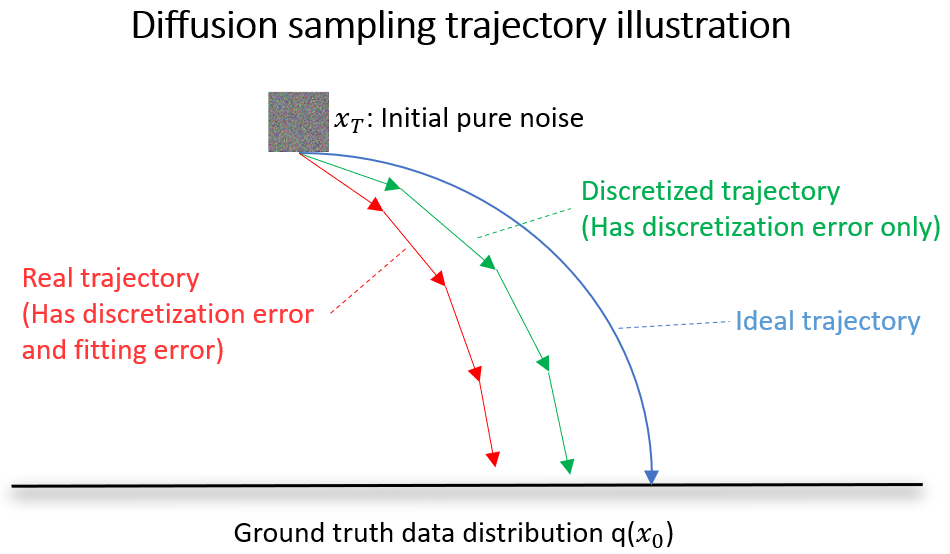
\includegraphics[width=0.45\textwidth]{figure/Error_discretization_vs_prediction.png}
\caption{Sampling trajectory illustration. In diffusion sampling process, there are two kinds of error: discretization error and fitting error. 
    The former happens when discretizing sampling process; and the latter is due to the mismatch between prediction and ground truth.}
\label{fig:error-d-vs-p}
\end{figure}

%============================================== Motivations
\section{Motivations}
Although new candidate technologies have been singled out for possible use in future aeronautical communications, the issue of spectral efficiency still continues to plague the aviation industry. Problems such as the coexistence of, and interference caused, by future and legacy communication systems on a crowded aeronautical spectrum are just a subset of potential issues which must be dealt with. Therefore, tackling the spectral crunch facing the aviation industry is a crucial but necessary step that must be taken in due time. Tackling the spectral efficiency issue will enable aeronautical communication links to better meet future data capacity demands while managing competition for spectral resources between current and future aeronautical communication technologies more efficiently. The urgency of improving spectral efficiency is also not unique to the aviation industry alone and is a challenging research problem in various other industries related to wireless communication systems \cite{dai2015non}. 

The study of spectral efficiency has always been a traditional problem in the communications literature. Related discussions, especially in recent years, have generally tackled the spectral efficiency problem from either a spectral utilization perspective or through employing advanced signal processing algorithms to exploit diversity advantages. Studies related to efficient spectrum utilization approaches have looked at various associated technologies such as Cognitive Radio (CR), enhanced modulation techniques and In-Band Full Duplex (IBFD) radio systems. Many others have also applied spectral efficiency techniques that have been studied in literature to a wide range of fields such as smart grids \cite{kouhdaragh2013cognitive}, wireless sensor networks \cite{he2014cr} and Long Term Evolution (LTE) networks \cite{zulhasnine2010efficient}. 

In terms of spectral efficiency for aeronautical communications, the application of LTE for A/G communications has been proposed in \cite{AlcatelSrat}. Concepts from the communications literature, such as adaptive modulations, have also been adopted for aeronautical usage in the form of AeroMACS \cite{budinger2011aeronautical}. However, the lack of available spectral resources is an underlying problem hampering further development of aeronautical communications technology. Therefore, more can be done in this aspect to further boost spectral efficiency for aeronautical communications.

%============================================== Objective of Work
\section{Objective of Work}
It is clear from the earlier discussions that the communication systems of both manned and unmanned aerial vehicles must utilize the limited aeronautical spectrum efficiently. One way to tackle the aeronautical spectrum crunch is to transmit more data per channel usage. Although an adaptive modulation-based ACS has been proposed in the form of AeroMACS \cite{budinger2011aeronautical}, modulation schemes that are suitable for aeronautical communications can also be studied to improve the data rate per channel usage, which is explored in the current work. To this end, the major milestones pertaining to suitable modulation schemes for aeronautical communications are summarized below.

%==============================================
\subsection{Major Milestones: Modulation Schemes}
\begin{itemize}
	\item The Quad State-Paired QPSK (QS-PQPSK), proposed in \cite{tan2016quad} to improve the data rate of current A/G links, was simulated for various aeronautical communications scenarios. In particular, the bit error rate (BER) of the QS-QPSK was compared against differential 8 phase shift keying (D8PSK) under  combinations of Rician and Rayleigh fading where it was found that the former outperforms the latter.
	\item To further improve the BER performance of QS-PQPSK, a Space Time Block Coded QS-PQPSK (STBC QS-PQPSK) was proposed. The BER of the proposed STBC QS-PQPSK was compared against 8PSK, QS-PQPSK and Rotative QPSK (RQPSK), i.e., bench marked against modulation schemes carrying three bits per symbol. In a Rayleigh flat fading channel, the proposed STBC QS-PQPSK outperforms 8PSK, QS-PQPSK and RQPSK across the simulated SNR ranges. 
	\item When simulated in the various aeronautical communications scenarios, the proposed STBC QS-PQPSK also exhibited superior BER performance when compared against QS-PQPSK and D8PSK.
\end{itemize}

Another alternative to tackle the aeronautical spectrum crunch directly is to transit from half-duplex (HD) based ACSs to hybrid-duplex (HBD) or even full-duplex (FD), i.e., IBFD, based ACSs. HBD-ACSs consist of HD and FD nodes concurrently operating on the same spectrum while FD ACSs requires all nodes to operate in FD mode. Therefore, both HBD-based and FD-based ACSs can provide up to twice the spectral efficiency when compared to existing /legacy HD-based ACSs.

As a step towards transitioning from HD-based ACSs to FD-based ACSs, HBD-based ACSs can be considered to minimize potential disruption to the aviation community. In particular, the current work evaluates the performance of an HBD-ACS from the outage and finite signal-to-noise-ratio (SNR) diversity-multiplexing tradeoff (DMT) perspective. The outage and finite SNR DMT analysis is used to identify suitable operating scenarios for which the HBD-ACS outperforms existing /legacy HD-based ACSs. The major milestones pertaining to HBD-ACS for aeronautical communications are summarized below.

%==============================================
\subsection{Major Milestones: HBD-ACS}
\begin{itemize}
	\item The present work proposes an innovative approach for deriving closed-form expressions for outage probability for a II detector and a two-stage SIC detector in a Rician faded environment.
	\item It is shown that the proposed HBD-ACS attains superior outage performance over existing HD-ACS at low SNRs. At high SNRs, however, the outage performance of the proposed HBD-ACS is eclipsed by HD-ACS as the former becomes interference-limited at asymptotic SNRs. Nonetheless, we show through numerical simulations that the HBD-ACS can meet typical Quality-of-Service (QoS) requirements, e.g., frame error rate $\leq 10^{-3}$, at high SNRs for a range of interference levels through II and SIC detectors. 
	\item Closed-form finite SNR diversity gain expressions are derived for the II and SIC detectors under Rician fading. The asymptotic behavior of the derived finite SNR diversity gains for HBD-ACS and HD-ACS are proven and shown to be consistent with interference-limited outage behaviors at asymptotic SNRs.
	\item The proposed HBD-ACS is shown to achieve better diversity gains than HD-ACS at high multiplexing gains. Finite SNR DMT analysis reveals that operating at higher multiplexing gain causes the Rician $K$ factor, corresponding to the SOI, to have more impact on HBD-ACS outage performance. Additionally, reducing residual SI and interference from AS-1 leads to steeper decay of outage probability, improving the finite SNR DMT curve of the proposed HBD-ACS as a consequence.
\end{itemize}
 
 %============================================== Report Outline
\section{Report Outline}

The remaining part of this report is organized as follows.

The state-of-the-art and suitable spectral efficiency techniques for aeronautical communications are discussed in Chapter II. In particular, future candidate technologies for various flight domains in aeronautical communications are presented as part of the state-of-the-art. Studies on aeronautical channel modeling are then presented, before further discussions on suitable spectral efficiency techniques for aeronautical communications 

In Chapter III, improvements to aeronautical waveforms over aeronautical communication channels are discussed. In particular, a new modulation scheme is proposed, simulated and compared, over various fading environments, against existing modulation schemes used in aeronautical communications.

Discussions on a proposed HBD system for aeronautical communications are presented in Chapter IV. The performance of the proposed HBD system is evaluated from both the outage probability and finite SNR DMT perspective, and is compared against existing HD systems.

Finally, future extensions of the works in Chapter III and Chapter IV are presented before the conclusion of this report in Chapter V.

%
%an overview of aeronautical communication links and systems in Chapter II. Discussions in Chapter II will span VHF-band (Very High Frequency-band), L-band and C-band systems for both A/G and A/A communication links. Channel access methods will also be briefly mentioned. We will then present suitable spectral efficiency techniques and its respective state-of-the-art that can be adopted for aeronautical communications in Section III. Finally, potential research topics will be deliberated in Section IV before the conclusion of this paper in Section V.
%
%This report is organized as follows:
%
%Chapter 2 provides ....................................
%
%Chapter 3 reviews ....................................
%
%Chapter 4 discusses ....................................
%
%In Chapter 5, we propose ....................................
%
%Finally, we conclude in Chapter 6, where we also discuss about the
%directions and schedule of our future research.
         % Include the chapters
%---------------------------------------------------------------------------------
\chapter{Denoising Diffusion Model: A Literature Review}
\label{chap:lit_review}
%---------------------------------------------------------------------------------
\section{Introduction}
To adequately cope with data communications demands, the aviation community have identified several candidate technologies for various flight domains. However, efficiently utilizing the aeronautical spectrum is still an issue, which can be addressed in the context of the following questions.

\begin{itemize}
	\item \textit{Which of the available spectral efficiency techniques can be adopted to improve spectral utilization in an aeronautical context?}
	\item \textit{How can the coexistence of legacy, existing and upcoming aeronautical communication technologies on a common aeronautical spectrum be managed?}
\end{itemize}

To this end, the state-of-the-art in aeronautical communications is first presented in this chapter. Thereafter, studies on aeronautical channel modeling are discussed. In particular, various propagation characteristics, e.g., fading scenarios, are present for different flight domains, which must be properly modeled to provide accurate analysis of any proposed aeronautical communication system (ACS). Suitable spectral efficiency techniques that can be adopted for aeronautical communications that are then presented and discussed from the aeronautical communications perspective.


\section{An Overview of Aeronautical Communications}
% brief history of aeronautical communications
Digital communication systems have long been employed in aeronautical communications for both A/A and A/G communication links. Early ACSs operated in the High Frequency (HF) band, rendering such systems to be susceptible to static and atmospheric noise \cite{stacey2008aeronautical}. Despite the development of Aircraft Communications Addressing and Reporting System (ACARS) and VHF digital link (VDL) from the late 1970's, HF ACSs e.g. HF-ACARS, are still retained \cite{stacey2008aeronautical}. This is because the propagation characteristics of the HF band enabled aircrafts to communicate over long distances in the absence of VHF coverage, particularly for flights over oceans or remote places. 

% motivations for FCI and the identified candidate technologies
Nonetheless, the aviation community has been on the search for newer generations of aeronautical data communication systems to adequately meet data communication demands in the near future. The joint European-American Future Communications Infrastructure (FCI) study, along with NextGen and SESAR as accompanying programs, is one such research initiative \cite{neji2013survey}. Specifically, the FCI study was tasked with recognizing possible communications technologies for future aeronautical communications over three phases. Phase one consists of identifying candidate technologies. Phase two concentrates on further adopting and adapting the selected candidate technologies for aeronautical applications and phase three culminates the FCI study with the implementation of required infrastructure on a global scale. It was noted in \cite{neji2013survey} at the time of publication that phase one had already been concluded, with a range of possible technologies identified. The RF bands used for different flight domains have also been identified. Flight domain in this sense refers to the type of terrain that the aircraft is operating in, e.g., when the aircraft travels on the airport/tarmac surface or fly over continental or remote places e.g. oceans, desert.

For surface communications i.e. airport/tarmac, AeroMACS was chosen \cite{neji2013survey,fistas2009future,ehammer2011aeromacs}. AeroMACS is an OFDM system with adaptive modulation based on the WiMAX standard, with data modulated either via QPSK, 16QAM or 64QAM depending on the link quality, i.e., Received Signal Strength Indicator (RSSI) \cite{budinger2011aeronautical,fistas2009future}. A feedback channel is also used to notify the transmitter of the link quality for the adaptive threshold decision process. When used in the C-band, the short range of AeroMACS signals in the C-band results in a high data rate communications platform with minimum interference. In particular, a performance evaluation of AeroMACS by Ehammer et al. \cite{ehammer2011aeromacs} revealed that for a fixed bit error rate (BER) of $10^{-6}$ and $5\times10^{-5}$, forward link bandwidth utilization of 1379 Kbps and 1738 Kbps were reported respectively. For the reverse link, bandwidth utilization of 684 Kbps and 812 Kbps were reported for a fixed BER of $10^{-6}$ and $5\times10^{-5}$ respectively. Separately, measurements conducted by Bundinger and Hall \cite{budinger2011aeronautical} as a test of the AeroMACS concept revealed an average of 3.89 Mbps to 5.13 Mbps of throughput. Despite noting that the airport surface environment is prone to multipath effects, theoretical channel models were not considered during the measurement tests by the authors.

For flights over remote places, the FCI study decided on satellite communication systems to operate in the L-band \cite{neji2013survey,morlet2011options}. These satellite communication systems are expected to be customized for aeronautical applications due to the inability of conventional or commercial satellite systems to support aeronautical communications \cite{neji2013survey}. One such example of a customized satellite communication system is the Iris program that is currently under development by the European Space Agency \cite{morlet2011options,morlet2010characterisation}. The aim of the Iris program is to enable satellite-based aeronautical communications as a complement to existing terrestrial-based ACSs such as LDACS since the former can cover a wider area than terrestrial-based ACSs \cite{morlet2011options}. Performance evaluation of the Iris program conducted by Morlet et al. \cite{morlet2010characterisation} revealed that for airport/tarmac and continental flight domains, an average throughput of 989 Kbps to 4.4 Mbps can be obtained for the forward link while an average throughput of between 568 Kbps to 728 Kbps can be obtained for the reverse link \cite{morlet2010characterisation}. In \cite{morlet2011options}, computer simulations were conducted for aircrafts operating in different regions (e.g. South and North Atlantic, Europe) and it was found that a maximum forward link throughput of 4.85 Mbps can be obtained. Although the Iris satellite communication system can be used to complement terrestrial ACSs, Morlet et al. \cite{morlet2011options} noted that the Iris satellite communication system can be susceptible to signal reception obstruction, i.e., airframe shadowing, which will be further discussed in the next section, due to aircraft maneuvers. This is on top of potential ground reflection of signals, thus causing multipath propagation effects.

Finally, for continental flights, candidates such as B-AMC and AMACS were noted by Neji et al. \cite{neji2013survey}. In the former, the adaptation of B-AMC for L-band communications was investigated in \cite{rokitansky2007bamc}. In the latter, an L-band All-purpose Multichannel Aviation Communication System (AMACS) based on VDL-4 and cellular GSM technology was considered \cite{eurocontrol2007amacs}, \cite{deneufchatel2007all}. Ultimately LDACS was chosen for continental aeronautical communications although satellite communication systems have not been ruled out completely \cite{neji2013survey}, \cite{fistas2009future}. The selected candidate technology and spectral band for the respective flight domains as part of the FCI study are summarized in Table \ref{table:aeroComms}. Note that the recommendations seen in Table \ref{table:aeroComms} have been agreed upon not only in Europe \cite{budinger2011aeronautical}, \cite{fistas2009future}, \cite{fistas2011future} but also in the United States as well \cite{wichgers2013study}, \cite{budinger2011aeronautical}, \cite{budinger2005technology}. 

%\begin{table}[]
%\centering
%\caption{Spectral bands and candidate technologies identified by the FCI study for various flight phases \cite{neji2013survey}, \cite{fistas2009future}}
%\label{table:aeroComms}
%\begin{tabular}{|p{5cm}|p{5cm}|p{2cm}|}
%\hline
%\textbf{Flight Domain}            & \textbf{Candidate Technology}          & \textbf{Spectral Band} \\ \hline
%Airport/Tarmac                    & AeroMACS                               & C-band                 \\ \hline
%Remote Places e.g. oceans, desert & Satellite Communication Systems        & L-band                 \\ \hline
%Continental                       & LDACS, Satellite Communication Systems & VHF and L-band         \\ \hline
%\end{tabular}
%\end{table}

\begin{table}[]
\centering
\caption{Spectral bands and candidate technologies identified by the FCI study for various flight phases \cite{neji2013survey}, \cite{fistas2009future}.} 
\label{table:aeroComms}\scalebox{0.85}{
\begin{tabular}{ccc}
\hline
\textbf{Flight Domain}            & \textbf{Candidate Technology}          & \textbf{Spectral Band} \\ \hline \hline
Airport/Tarmac                    & AeroMACS                               & C-band                 \\ 
Remote Places, e.g., oceans, desert & Satellite Communication Systems        & L-band                 \\ 
Continental                       & LDACS, Satellite Communication Systems & VHF and L-band         \\ \hline
\end{tabular}}
\end{table}

As a result of the FCI study, continental communications via LDACS has seen gradual increase in research interest. This is because LDACS must be able to handle the tremendous volume of aircrafts communicating on A/G links. In addition, the choice between the two variants of LDACS namely LDACS-1 and LDACS-2, is yet to be made \cite{jain2011analysis}. Although both operate in the L-band at the physical layer, LDACS-1 is based on FDD-OFDM that adaptively switches between QPSK, 16-QAM and 64-QAM modulation on a 498KHz channel \cite{brandes2009physical}. This is on top of adaptive convolutional coding that chooses between 1/2, 2/3 or 3/4 code rate. Thus, LDACS-1 can provide up to 1373Kbps and 1038Kbps in the forward and reverse link respectively \cite{jain2011analysis}, \cite{brandes2009physical}. LDACS-2, based on GSM and AMACS, uses GMSK modulation with TDD for multiuser access \cite{neji2013survey}, \cite{fistas2009future}, \cite{jain2011analysis}, \cite{abdulkarim2013comparison}. Using GMSK, LDACS-2 is able to provide 270Kbps of raw throughput with a bandwidth of 200 KHz \cite{jain2011analysis}. This is lower than that of LDACS-1 which requires close to 500 KHz. In terms of spectral efficiency, Jain et al. \cite{jain2011analysis} noted that LDACS-1 can support up to 2.76 bits/s/Hz and 2.08 bits/s/Hz for forward and reverse links respectively. For LDACS-2, 1.3 bits/s/Hz was reported although this number may be lower when coding and overhead costs are considered \cite{jain2011analysis}.

Invariably, LDACS-1 will be able to provide higher data rate communications at a cost of higher spectral resource requirements. Conversely, LDACS-2 will require less spectral resources albeit at lower data rate communications. Evidently, evaluation studies between LDACS-1 and LDACS-2 are already being carried out \cite{neji2013survey}, with the specifications of LDACS-1 and LDACS-2, appropriate prototype developments, e.g., via simulator frameworks such as in \cite{graupl2015method}, aeronautical channel modeling and most crucially, potential interference from existing L-band legacy systems \cite{neji2013survey}, \cite{jain2011analysis}, \cite{brandes2009physical} \cite{epple2014overview} being taken into consideration. These legacy systems include Distance Measurement Equipment (DME), Tactical Air Navigation (TACAN), Universal Access Transceiver (UAT), Secondary Surveillance Radar (SSR), satellite systems, e.g., Global Positioning System (GPS), and telecommunication standards, such as Global Systems for Mobile (GSM) communications and Universal Mobile Telecommunications System (UMTS) \cite{neji2013survey}, \cite{epple2014overview}. Of these systems, Jain et al. \cite{jain2011analysis} noted strong interference from DMEs and telecommunication equipments. In particular, Jamal and Matolak \cite{jamal2017fbmc} showed that interference from DMEs and telecommunication equipments can be detrimental, especially to wideband systems such as LDACS-1. 

Improvements to the proposed LDACS-1 system have also been studied. For instance, Brandes et al. \cite{brandes2009physical} proposed oversampling and zero-padding (referred to as Pulse Blanking in \cite{brandes2009physical}) to mitigate interference from legacy systems. However, this reduces the overall throughput. Similarly, works such as \cite{bhaindl2013overview} and \cite{mschnell2014current} have proposed to extend LDACS-1 for navigational purposes to replace navigation systems in a bid to reduce congestion on the L-band. The adaptation of LDACS-1 as an Alternative Positioning, Navigation and Timing (APNT) solution was presented by Schnell et al. \cite{schnell2011using}. Based on signal latency, the relative distance between aircraft and ground station can be estimated via symbol synchronization. In addition to distance, an aircraft's position can also be estimated (via Weighted Least Squares or Extended Kalman Filter) once the distance to at least three ground stations has been estimated. Accuracies of up to 100m have been reported by using the proposed navigation methods. 

Apart from manned A/G communications, LDACS has also been considered for UAV CNPC links. For instance, Matolak \cite{matolak2015unmanned} cited LDACS-1 and LDACS-2 as potential candidates for future CNPC systems. In terms of future ACSs for A/A communications, Schnell et al. \cite{schnell2014ldacs} noted that this was beyond the scope of both SESAR and NextGen although ADS-B might be a possible future A/A communications technology. Nonetheless, despite LDACS being the selected candidate technology for continental A/G communication links, issues such as standardization, interference management and spectral resource allocation are crucial challenges \cite{neji2013survey} that must be tackled by the aviation community in due time. A summary of the studies that have conducted performance evaluations on the candidate technologies can be seen in Table \ref{table:sumCandidateTech}.

\begin{table}[]
\centering
\caption{Performance evaluation studies conducted for candidate technologies}
\label{table:sumCandidateTech}
\scalebox{0.9}{
\begin{tabular}{ccc}
\hline
\textbf{Candidate Technology}   			& \textbf{Performance Metric(s)}  			& \textbf{References} 							\\ \hline \hline
AeroMACS                    					& Throughput 									& \cite{budinger2011aeronautical} 	\\ 
AeroMACS                    					& Throughput 									& \cite{ehammer2011aeromacs}  			\\ 
Satellite Communication System (Iris)	& Throughput, Antenna Gain    & \cite{morlet2011options}        	\\ 
Satellite Communication System (Iris)	& Throughput                  & \cite{morlet2010characterisation} \\ 
LDACS	1, LDACS-2	                    & Throughput                  & \cite{jain2011analysis}           \\ 
LDACS	1, LDACS-2	                    & BER, Power Spectral Density & \cite{jamal2017fbmc}        \\ 
LDACS	1	                    					& Latency, Packet Loss Rate   & \cite{graupl2015method}           \\ 
LDACS	1	                    					& BER													& \cite{brandes2009physical}        \\ \hline
\end{tabular}}
\end{table}

\section{Aeronautical Channel Modeling}
The characterization of accurate aeronautical channel models for common A/G and A/A communications scenarios has been extensively studied in the literature. Statistical channel models for A/G communications was studied by Haas \cite{haas2002aeronautical}. The study involved analyzing the channel model of an aircraft communicating with a ground station in en route, arrival/takeoff, taxi and parking scenarios, as seen in Table \ref{table:haasFading}. 

\begin{table}[]
\centering
\caption{Fading environments for the various flight scenarios \cite{haas2002aeronautical}.} 
\label{table:haasFading}\scalebox{0.9}{
\begin{tabular}{ccc}
\hline
\textbf{Flight Scenario}				& \textbf{Fading Environment(s)}	& \textbf{Average Rician $K$ Factor} \\ \hline \hline
En route												& Rician and Rayleigh 						& $15dB$ \\
Arrival/Takeoff 								& Rician and Rayleigh 						& $15dB$ \\
Taxi														& Rician and Rayleigh 						& $6.9dB$ \\
Parking                 				& Rayleigh 												& - \\ \hline
\end{tabular}}
\end{table}

The en route scenario can be characterized by an aircraft communicating with a ground station while at cruising altitude with a speed of 17m/s to 440m/s. The arrival/takeoff scenario can be characterized by A/G communications between an aircraft and ground station during landing or takeoff with a speed of 25m/s to 150 m/s. For both the en route and arrival/takeoff scenarios, Rician and Rayleigh fading are assumed for the line-of-sight (LOS) and non line-of-sight (NLOS) components respectively with an average $K$ factor of 15dB. The taxi scenario occurs when an aircraft is communicating with a ground station while traveling on the airport surface with a speed of 0m/s to 15m/s. In this scenario, Rician and Rayleigh fading are also assumed for the LOS and NLOS components respectively with an average $K$ factor of 6.9dB. Finally, the parking scenario occurs when an aircraft is stationary on the airport surface. In this scenario, Haas \cite{haas2002aeronautical} assumed only NLOS communications between aircraft and ground station thus Rayleigh fading is assumed in the parking scenario.

Apart from Haas \cite{haas2002aeronautical}, other recent works on aeronautical channel models have been noted. The propagation characteristics of C-band and L-band signal in A/G communications over water, hilly terrains and suburban/near-urban areas have been investigated as a series of papers in \cite{matolak2017air_water},\cite{sun2017air_hilly} and \cite{matolak2017air_suburban} respectively. In each of these studies, measurements were taken by conducting A/G communications with a ground station when the aircraft is flying over the respective terrains. 

For A/G communications over water surfaces, Matolak and Sun \cite{matolak2017air_water} reported that the free space path loss model can be used to model signal propagation effects, with path loss exponents between 1.5 to 2.2 observed. However, at distances of 10km and above, signal measurements showed that the curved earth two-ray model fits the data more accurately due to water surface reflections. To this end, it was found that the respective $K$ factor for both the L-band and C-band signals are 12dB and 27 to 30dB. Other than Matolak and Sun \cite{matolak2017air_water}, an earlier study by Meng and Lee \cite{meng2011measurements} also reported that the two-ray model can be accurately used to model C-band signal propagation over water surfaces.

The study in \cite{matolak2017air_water} was extended to hilly terrains by Sun and Matolak \cite{sun2017air_hilly}. It was found that, by taking the direction of the aircraft (heading towards or away from ground station) into consideration, the modified log-distance path loss model was able to fit the measured signal accurately. To this end, path loss exponents between 1.6 to 1.8 was observed. From the analysis of the signal measurements, it was also reported that signal reflections from hilly terrain follow a Rician distribution, with an average $K$ factor of 29.4dB and 12.8dB for C-band and L-band respectively.

For A/G communications on airport surface or over suburban/near-urban areas, observations similar to those in \cite{sun2017air_hilly} was reported by Matolak and Sun \cite{matolak2017air_suburban}. Notably, signal propagation path losses in suburban/near-urban areas followed the modified log-distance path loss model with path loss exponents between 1.5 to 2 was observed. For near-urban area, an average $K$ factor of 27.4dB and 12dB was observed for C-band and L-band respectively. In suburban areas, the average observed $K$ factor values for C-band and L-band are 28.5dB and 14dB was observed for C-band and L-band respectively. For airport surface communications, Wu et al. \cite{wu2011airport} observed that the two-ray or log-distance model can accurate model path loss, with an average path loss exponent of 4 and 5.6 reported for the LOS and NLOS components respectively. 

In addition to the studies conducted in \cite{matolak2017air_water}, \cite{sun2017air_hilly}, \cite{matolak2017air_suburban}, the effect of airframe shadowing on A/G communication channels was also recently investigated by Sun et al \cite{sun2017air_shadowing}. Airframe shadowing occurs when an aircraft's body temporarily obstructs the LOS A/G channel between the aircraft and the ground station due to aircraft maneuvers. Sun et al \cite{sun2017air_shadowing} was able to model airframe shadowing loss as a function of an aircraft's roll angle. Signal measurements revealed that an average path loss of 15.5 dB and 10.8 dB for C-band and L-band signals. In addition, it was also observed that airframe shadowing can significantly reduce the Rician $K$ factor for LOS components, with measurements showing a drop of up to 35dB. Furthermore, Sun et al \cite{sun2017air_shadowing} reported that airframe shadowing losses are independent of the link distance and ground station environment. Airframe shadowing can be mitigated by placing additional antennas on the aircraft to maintain LOS A/G communication \cite{sun2017air_shadowing}. However, future ACSs will need to explore other practical solutions because the option of having additional antenna mounting points may not always be available.

\begin{table}[]
\centering
\caption{A summary of propagation environments over various types of terrain.} 
\label{table:propTerrain}\scalebox{0.8}{
\begin{tabular}{ccc}
\hline
\textbf{Terrain}					& \textbf{Average Rician $K$ Factor} 					& \textbf{Path Loss Exponent} \\ \hline \hline
Water Surfaces						& 12dB (L-band), 27dB-30dB (C-band) 					& 1.5 - 2.2 \\
Hilly 										& 29.4dB (C-band), 12.8dB (L-band) 						& 1.6 - 1.8 \\
Airport or Urban/Suburban & 27.4dB-28.5dB (C-band), 12dB-14dB (L-band) 	& 1.5 - 2 \\ \hline
\end{tabular}}
\end{table}

In this section, discussion on accurate modeling of aeronautical channels have been presented. In particular, combinations of Rician and Rayleigh fading are commonly encountered aeronautical communications. Important parameters, such as Rician $K$ factors and path loss exponents, have been characterized by various studies for different scenarios/terrains, as summarized in Table \ref{table:haasFading} and Table \ref{table:propTerrain}. It should also be pointed out that the signal models for various aeronautical scenarios in the current work are based on the parameters in Table \ref{table:haasFading} and Table \ref{table:propTerrain}.

%%%%%%%%%%%%%%%%%%%%%%%%%%%%%%%%%%%%%%%%%%%%%%%%%%%%%%%%%%%%%%%%%%%%%%%%%%%%%%%%%%%%%%%%%%%%%%%%%%%%%%%%%%%%%%%%%%%%%%%%%%%%%%%%%%%%%%%%%%
\section{Potential Spectral Efficiency Techniques in Aeronautical Communications}

Spectral efficiency improvements have long been a topic of interest in the literature, with many techniques that can be potentially adopted for aeronautical communications. For instance, the CR paradigm can be applied for ACSs in A/G communications scenarios. In A/G communications scenarios, legacy ACSs on board aircrafts can continue to operate in the designated spectrum as primary users while allowing newer generations of communication systems to operate as secondary users in overlay (interweave) mode \cite{jacobcognitive}. Such an arrangement can keep interference to legacy systems in check while accommodating newer generations of ACSs on board aircrafts. 

The cognitive radio paradigm can also be adopted for A/A communications between aircrafts (manned or unmanned) in the form of Device-to-Device (D2D) communications. D2D communications can be used to relay signals between nearby aircrafts and ground stations for interference cancellation. Therefore, the quality of A/A and even A/G communications is improved while potential interference from legacy ACSs is reduced. When combined with proper spectrum access management, i.e., CR-based techniques seen in \cite{min2011capacity}, \cite{chen2012downlink}, \cite{xu2014dynamic}, an A/A D2D communications system can also be used for data communications over oceanic or polar flight routes where A/G communications is not possible via signal relaying between aircrafts.

\begin{figure}[]
\centering
\vspace{-2cm}
\includegraphics [width=0.8\columnwidth]{chap2_fig/chap2_fd_gs_system_model.eps} 
\vspace{-2.2cm}
\caption{Multi-user system model with a FD ground station and (a) HD receivers or (b) FD receivers.}
%\vspace{-0.5cm}
\label{fig:chap2_fd_gs_system_model}
\end{figure}

\begin{figure}[]
\centering
\vspace{-2cm}
\includegraphics [width=0.8\columnwidth]{chap2_fig/chap2_hd_gs_system_model.eps} 
\vspace{-2cm}
\caption{Multi-user system model with a HD ground station and (a) HD receivers or (b) FD receivers.}
%\vspace{-0.5cm}
\label{fig:chap2_hd_gs_system_model}
\end{figure}

Apart from the techniques discussed earlier, several other spectral efficiency techniques, suitable for aeronautical communications, are available in the literature. However, the current work focuses on improving spectral efficiency in HD and FD-enabled ACSs over A/G links. In HD ACSs, the system model in Fig. \ref{fig:chap2_hd_gs_system_model}a is assumed, where the HD ACS, i.e., avionics, communicates with the ground station (GS). In FD ACSs, as seen in Fig. \ref{fig:chap2_fd_gs_system_model} and Fig. \ref{fig:chap2_hd_gs_system_model}b, self interference (SI) is experienced at the the FD transceivers due to the simultaneous signal transmission and reception. Also, interference at both HD and FD ACSs is also experienced due to the uplink nature of communication. 

Based on the system models seen in Fig. \ref{fig:chap2_fd_gs_system_model} and Fig. \ref{fig:chap2_hd_gs_system_model}, the current work focuses on advanced modulation schemes and In-Band Full-Duplex radio systems to boost spectral efficiency in HD and FD-enabled ACSs, which are practical and efficient spectrum utilization alternatives in aeronautical communications and is discussed in detail in the subsequent subsections.

\subsection{Modulation and Multiplexing Schemes for Aeronautical Communications}
\subsubsection{Modulation Schemes for Aeronautical Communications} 
% Disscuss relevance to aeronautical communications
Current A/G links rely on VDL-2 for data communications. However, the VDL-2 specification employs D8PSK as the modulation of choice to provide for a data rate of 31.5 kbps \cite{stacey2008aeronautical}. Evidently, the achievable data rate of VDL-2 is woefully inadequate if future data communication demands are to be met. To address the low data rate issue of current A/G links, advanced modulation schemes suitable for aeronautical communications can be implemented that either increases the number of bits transmitted per symbol or improves the reliability of communications, i.e., boost the spectral efficiency of ACSs. 

% Discuss techniques that increases the number of bits per transmitted symbol
The hierarchical modulation paradigm has been explored as an alternative to increase the number of bits per transmitted symbol by relying on the quadrant containing the QAM symbol as an additional domain to represent data bits \cite{jiang2005hierarchical,bae2008research} at the cost of signal detection complexity. Modified variants of PSK-based modulation have also been studied to increase the bits carried per symbol. In particular, transmitting additional bits through rotating the QPSK constellation in a specific direction was proposed by Liu et al. \cite{liu1992rotative}. Through the proposed method, an additional bit can be transmitted per QPSK symbol at the cost of higher receiver complexity. More recently, Hong et al. \cite{hong2015additional} proposed rotating the QPSK constellation after the transmission of each block of bits to convey additional bits. Although the detection complexity is not as substantial compared to \cite{liu1992rotative}, the proposed method only achieves a maximum of 16\% boost in throughput.

% Discuss BICM and SSD as techniques that increases reliability
% Present open problems related to aeronautical communications if possible
Apart from increasing transmission rates, enhanced modulation techniques have also been extensively studied to improve reliability. For instance, Bit Interleaved Coded Modulation (BICM) was first proposed by \cite{zehavi19928} to improve the reliability transmissions over Rayliegh fading channels. In particular, the transmitter performs interleaving at the bit level before modulation and vice versa at the receiver \cite{zehavi19928,caire1998bit,li2002bit,zhan2017differential}. BICM has since been extensively studied, with different decoding methods proposed \cite{li2002bit,abotabl2017broadcast} and evaluation over multipath Rayleigh channels conducted \cite{zhan2017differential}. Nonetheless, the increase in reliability for BICM comes at the cost of reduced euclidean distance \cite{li2002bit}.

Signal Space Diversity (SSD), i.e., modulation diversity, is also another technique that has been widely studied to improve communications reliability. SSD was first proposed by Boutros and Viterbo \cite{boutros1998signal} where the in-phase and quadrature phase components of a symbol are rotated and interleaved. The idea is to separately transmit the in-phase and quadrature phase components over a fading channel to diminish the impact of fading \cite{boutros1998signal}. By far, studies pertaining to SSD have looked at code design \cite{mohammed2012modulation} and performance analysis over Nakagami-$m$ \cite{lu2012bit} and Rayleigh \cite{sokun2017spectrally} fading channels. These analysis are useful since Nakagami-$m$ and Rayleigh can be encountered in aeronautical communications. However, suitable code designs for aeronautical communications and the impact of imperfect channel knowledge, particularly for various flight scenarios where Rician fading channels are expected, are open problems that must be addressed.

\subsubsection{Multiplexing Schemes for Aeronautical Communications}

An alternative to meet demands for rising data traffic stemming from aeronautical communications is the non-orthogonal multiple access (NOMA) paradigm. NOMA has been proposed as a next-generation multiple access candidate \cite{dai2015non} in 5G cellular communications. As spectral efficiency is a vital issue that must be addressed in 5G, NOMA, when compared to orthogonal multiple access (OMA) methods, offers spectral efficiency boosts whilst allowing massive connectivity \cite{dai2015non}. Conventional OMA methods such as Frequency Division Multiple Access (FDMA), Time Division Multiple Access (TDMA) and Code Division Multiple Access (CDMA) have traditionally been used to segregate users in terms of channel frequencies (e.g. spectral resources), timeslots or codes. 

However, OMA techniques inherently causes inefficient utilization of spectral resources as users have dedicated resources at the moment of transmitting or receiving signals. NOMA, on the other hand, allows multiple users to simultaneously share the same spectral resources. This is done by allowing an acceptable amount of interference from users simultaneously multiplexed to the same set of spectral resources \cite{dai2015non}. The NOMA paradigm can be well suited for adaptation for aeronautical communications. Interference from nearby aircrafts or ground stations can be canceled while accommodating a large number of aircrafts in the same airspace that are transmitting data via A/G or A/A communication links. To enable resource multiplexing, NOMA techniques can be broadly categorized as Power Domain Multiplexing (PDM) or Code Domain Multiplexing (CDM). 

\begin{figure} []
\centering
\vspace{-0.7in}
\includegraphics [width=0.6\columnwidth]{chap2_fig/NOMA_fig1.eps}  %ZICRSystemModel.eps} % {LAR.eps}\columnwidth   [width=2\columnwidth] 
\vspace{-0.8in}
\caption{Users in power domain multiplexing are partitioned using transmission power levels.}
\label{fig:6}
\end{figure}

In PDM-NOMA, signals are transmitted on the same frequencies using different power levels (Fig. \ref{fig:6}). This method of PDM is known as basic NOMA and was discussed by Saito et al. in \cite{saito2013non}. In particular, basic NOMA was applied for a downlink scenario involving two users, user one and user two with message signals $x_1$ and $x_2$ respectively and one base station. The base station transmits signal $y=x_1+x_2$ to all users simultaneously, with the sum of the transmit powers subjected to power constraints. To recover the signals, the users employ Successive Interference Cancellation (SIC) \cite{saito2013non}. 

Assuming that user 1 has less interference than user 2, user 1 will recover $x_1$ before subtracting $x_1$ from $y$. User 2 will then recover $x_2$ from $y$ after user one recovers $x_1$ \cite{saito2013non}. In general, SIC is used by users for signal detection, based on SINR measurements that is relative to all other nearby users. It was noted by Saito et al. \cite{saito2013non} that the power allocation ratio affects effective user throughput. To address this, flexible RRM is needed to take full advantage of this PDM technique. Similarly, Higuchi and Kishiyama \cite{higuchi2013non} proposed a beamforming PDM technique for MIMO LTE networks. In particular, the proposed technique combined beamforming and SIC for PDM-NOMA. It was however, noted by Song and Wang \cite{song2016comparison} that the main problems concerning SIC is the user delay and the potentially severe error propagation.

In contrast, techniques based on CDMA have been adopted for CDM-NOMA. One such method is Low Density Signature (LDS), seen in a paper by Hoshyar et al. \cite{hoshyar2008novel}. LDS is based on the LDPC spreading technique, that was originally developed for CDMA. The key idea behind LDS is to use sparse spreading sequences to reduce chip interference \cite{dai2015non}, {yuan2016non}. This is in contrast to dense spreading used in CDMA and is the key difference between LDS-based CDM-NOMA and conventional CDMA. In LDS, users recover their own messages by via a message passing algorithm (MPA) \cite{dai2015non}. Apart from LDS, Sparse Code Multiple Access (SCMA) has been explored as an alternative to LDS for CDM-NOMA by Nikopour and Baligh \cite{nikopour2013sparse}. Similar to LDS, SCMA relies on sparsely populated code words form via multi-dimensional constellations for non-orthogonal access \cite{yuan2016non}. Specifically, each user is assigned a sparsely coded codebook and data streams from each user are encoded via the respective codebooks before transmission. At the receiver, user detection is achieved via a MPA. Although both LDS and SCMA enable multi-user non-orthogonal access, the main limitation of both techniques is scalability \cite{yuan2016multi}.

\begin{figure} [!htpb]
\centering
\vspace{-0.6in}
\includegraphics [width=1\columnwidth]{chap2_fig/NOMA_fig2.eps}  %ZICRSystemModel.eps} % {LAR.eps}\columnwidth   [width=2\columnwidth] 
\vspace{-1.5in}
\caption{A complex valued codeword constellation with 4 elements in MUSA. \cite{yuan2016multi}}
\label{fig:noma_fig2}
\end{figure}

An alternative for CDM-NOMA is Multi User Shared Access (MUSA), which was  in \cite{dai2015non}, \cite{yuan2016multi}. In MUSA, short length complex-valued codewords are used to spread user signals before transmission  \cite{yuan2016multi}. The complex valued codewords are constructed from complex valued constellations, with each codeword element picked from the constellation (Fig. \ref{fig:noma_fig2}). User overloading is thus accomplished by increasing the length of the codeword. For a codeword with length of $K$, there will be $4^K$ codewords available thus enabling scalability \cite{yuan2016non}. At the receiver, codeword-level SIC is employed to differentiate user messages. Although MUSA is more scalable then LDS and SCMA, the message recovery process in MUSA introduces the risk of error propagation due to SIC at the receiver. A summary of the discussed NOMA approaches is presented in Table \ref{table:noma}.

\begin{table}[]
\centering
\caption{Summary of discussed NOMA approaches}
\label{table:noma} \scalebox{0.9}{
\begin{tabular}{ccc}
\hline
\textbf{References}					& \textbf{Description}		 			& \textbf{Spectral Efficiency Metric(s)} \\ \hline \hline
\cite{saito2013non} 				& Basic NOMA SIC for PDM-NOMA   & Throughput                             \\ 
\cite{higuchi2013non}       & Beamforming SIC for PDM-NOMA  & Throughput                  \\ 
\cite{hoshyar2008novel}			& LDS for CDM-NOMA							& BER                                    \\
\cite{nikopour2013sparse}		& SCMA for CDM-NOMA							& BER                                    \\
\cite{yuan2016multi}				& MUSA for CDM-NOMA							& BER                                    \\ \hline
\end{tabular}}
\end{table}

%Non-Orthogonal Multiple Access (NOMA), on the other hand, is an alternative technique that can be adopted for spectral efficiency improvements in aeronautical communications. NOMA has been proposed as a next-generation multiple access candidate \cite{dai2015non} in 5G cellular communications. As spectral efficiency is a vital issue that must be addressed in 5G, NOMA, when compared to OMA methods, offers spectral efficiency boosts whilst allowing massive connectivity \cite{dai2015non}.
%
%NOMA allows multiple users to simultaneously share the same spectral resources by allowing an acceptable amount of interference from users simultaneously multiplexed to the same set of spectral resources \cite{dai2015non}. To enable resource multiplexing, NOMA techniques can be broadly categorized as Power Domain Multiplexing (PDM) or Code Domain Multiplexing (CDM).
%
%The NOMA paradigm can be well suited for adaptation for aeronautical communications. PDM-NOMA for instance, can take advantage of the fact that aircrafts on a flight path can be separated by vast distances (e.g. 10km and above). When path loss is considered, interfering signals from nearby aircrafts or ground stations is diminished. Thus, PDM-NOMA can be adopted for both A/G and A/A communications scenarios. CDM-NOMA can also be adopted for aeronautical communications, particularly in congested airspace where a large number of aircrafts are transmitting data via A/G or A/A communication links. In such a scenario, spectral efficiency is improved through simultaneous transmissions achieved via Multi User Shared Access (MUSA) \cite{dai2015non}, \cite{yuan2016multi} or even Sparse Code Multiple Access (SCMA) \cite{nikopour2013sparse}. Interference with legacy aeronautical communications can also be managed if PDM-NOMA or CDM-NOMA techniques are used in combination with D2D/CR related approaches.

\subsubsection{Open Research Problems for Modulation and Multiplexing Schemes in Aeronautical Communications}

The spectral efficiency of ACSs can be improved through suitable modulation schemes. With the current VDL-2 scheme providing low data rates for A/G links, modulation techniques that can transmit more bits per symbol effectively, with simple transceiver designs, can be further investigated. BICM can also be further explored for aeronautical communications usage. In particular, performance analysis of BICM over multipath channels are limited \cite{zhan2017differential}, particularly for combinations of Rician and Rayleigh fading which are expected in aeronautical communications, and can be studied in future works. For SSD, code designs that are suitable for aeronautical communications and the impact of imperfect channel knowledge, particularly for various flight scenarios where Rician fading channels are expected, are also open research problems that must be addressed.

NOMA approaches can also go a long way towards improving the spectral efficiency of ACSs. Although concepts such as frequency reuse, have been applied for aeronautical communications e.g. VDL-2 systems \cite{ribeiro2014framework}, there is further scope to study the feasibility of new NOMA methods for aeronautical communications. By enabling simultaneous sharing of the same frequency band, NOMA provides the capability to support simultaneous transmissions from multiple users in the same channel. When applied to ACSs, NOMA can effectively help to address the scarcity of aeronautical spectrum for communications. 

However, the major downside to such an approach is the inevitable introduction of interference to all NOMA users. In the aeronautical context, this translates to interfering with A/G or even A/A communications. In the worst case, the transmissions of legacy systems in the same band e.g. VHF or L-band, can also be affected. In this aspect, much work will have to be done in the aeronautical context to quantify potential levels of interference to other aircrafts and legacy systems. This is on top of improving PDM-NOMA or CDM-NOMA techniques to reduce delays, error propagation and complexity, which are still open research problems. Finally, future work can also for instance, study the feasibility of incorporating frequency reuse into PDM-NOMA for aeronautical communications.

\subsection{In-Band Full-Duplex Radio Systems for Aeronautical Communications}

% Disscuss relevance to aeronautical communications
The emerging field of In-Band Full-Duplex (IBFD) radio systems can be a direct solution to improve the spectral crunch faced by the aviation community. From the aeronautical communications perspective, IBFD systems enable ACSs, e.g., VDL-2, AeroMACS, LDACS-1 or LDACS-2, the capability to simultaneously transmit and receive signals on the same channel. Therefore, ACSs operating in FD mode can achieve up to twice the spectral efficiency compared to operating in HD mode. Furthermore with proper signal processing techniques, interference and congestion on the aeronautical spectrum between legacy, existing and FD-enabled ACSs can be managed. However, many technical challenges related to interference cancellation/management must be tackled before any aeronautical IBFD communications system can be made feasible.

\subsubsection{SI Cancellation Architectures and the Associated Considerations in Aeronautical Communications}
% Discuss SI technical hurdle and related SI cancellation literature in FD systems
\begin{figure} []
\centering
\vspace{-0.7in}
\includegraphics [width=0.7\columnwidth]{chap2_fig/IBFD_fig2.eps} 
\vspace{-0.8in}
\caption{Overview of SI mitigation architectures. \cite{sahai2013impact}.}
\label{fig:IBFD_2}
\end{figure}

One of the major technical hurdles in IBFD systems is the inherent introduction of self interference (SI). A practical IBFD system requires a sufficient level of SI mitigation before communications can become feasible. In this aspect, SI mitigation architectures can be categorized into either passive suppression or active cancellation \cite{sahai2013impact} (Fig. \ref{fig:IBFD_2}). The former entails SI mitigation via antenna separation (separate antenna IBFD systems) \cite{duarte2014design,ahmed2012simultaneous} or circulator isolation (shared antenna IBFD systems) \cite{bharadia2013full,huberman2015mimo} while the latter cancels SI either in the analog or digital domain. 

Active analog/digital SI cancellation architectures are further categorized as pre-mixer, post-mixer or baseband cancelers. A mixture of pre, post and baseband cancelers in the same architecture is also possible. In a pre-mixer canceler, the processing of the cancellation signal is performed before the RF mixer, e.g., having a parallel radio chain \cite{ahmed2015all}. Likewise, a post-mixer canceler processes the cancellation signal after the RF mixer, e.g., Balun (Balance/Unbalance) cancellation \cite{jain2011practical} while a baseband canceler processes the canceling signal at the baseband level.

% Discuss open problems related to SI mitigation
It should be noted that digital and analog SI cancellation both experience unique limitations \cite{sahai2013impact}. In digital SI cancellation, the strength of the resultant SI signal before it enters the ADC is high. Consequently, SI mitigation becomes ineffective since the SI signal will still be above the receiver noise floor after digital SI cancellation due to limited ADC dynamic range \cite{sabharwal2014band}. In analog SI cancellation, SI mitigation will require complex hardware \cite{everett2016softnull}, thus potentially increasing the physical size of transceivers and contributing to overall size, weight and power requirements for FD-enabled avionics. 

On top of the associated limitations for both digital and analog SI cancellation, residual SI will also be present in the form of phase noise. The residual SI is a result of imperfect SI channel estimation at the FD transceiver \cite{sahai2013impact} and it can be the limiting factor in practical IBFD systems. In addition, suitable SI mitigation architectures of IBFD systems (e.g. active or passive) will need to be investigated to determine a suitable architecture for aeronautical usage, on top of accurate theoretical modeling of SI signals and multipath fading effects in an aeronautical channel e.g. Rician or Rayleigh fading environments \cite{haas2002aeronautical}.

\subsubsection{Hybrid-Duplex Systems for Aeronautical Communications}
% Discuss HBD systems as a way to transition towards a newer generation of FD-enabled ACSs
Apart from suitable SI mitigation architectures and the associated considerations for aeronautical communications, transiting towards a new generation of FD-enabled ACSs is likely to be disruptive as legacy HD ACSs must first be replaced. To ease the transition from legacy HD to a FD-enabled ACS, a hybrid-duplex (HBD) ACS consisting of HD and FD aircrafts/ground stations, e.g., Fig. \ref{fig:chap2_fd_gs_system_model}, is a viable alternative. 

Already, HBD systems have been seen in cognitive radio systems \cite{li2014linear} and cellular systems \cite{yin2013full,jang2015spatial,cirik2016robust} where nodes operating in either HD or FD have been studied. The main obstacle in such a HBD system is the inherent SI as a result of simultaneous signal transmission and reception. As a result, sufficient levels of SI mitigation must be achieved to enable the co-existence of multiple ACSs operating on the same frequency. In this aspect, concepts related to NOMA can be adapted for FD operations. Future studies can look at the suitability of incorporating Successive Interference Cancellation (SIC) from power-domain NOMA \cite{yan2015receiver}, \cite{huang2016full}, \cite{ali2016dynamic}, \cite{zhang2016full} into multi-user IBFD wireless systems. Other studies can also look at using code-domain NOMA concepts such as MUSA or SCMA \cite{yuan2016multi}, \cite{nikopour2013sparse}. 

Apart from SI, HBD systems must also manage interference from nearby HD nodes, e.g., HD avionics, as seen in Fig. \ref{fig:chap2_fd_gs_system_model}a. Interference management strategies have long been an area of active research in the literature, particularly from the information theoretic perspective. For instance, studies investigating interference management approaches that do not consider any inherent structure in the interference, such as interference avoidance, have been noted \cite{qu2014understanding}. Such interference avoidance strategies, which are typically based on either random access, e.g., contention-based channel access, or deterministic access, e.g., orthogonal multiple access, hinders spectral efficiency \cite{qu2014understanding,weber2007transmission}. Therefore, exploiting the structure of interference, i.e., interference management, has been the topic of keen research interest in recent years \cite{qu2014understanding} to achieve better performance \cite{weber2007transmission} and spectral efficiency in multi-user systems. 

In aeronautical communications, the distances between aircrafts affects the level of interference experienced at the HD avionics. Long separation distances between aircrafts results in weak interference scenarios and vice-versa. Accordingly, suitable interference management techniques must be employed for different interference scenarios. For weak interference scenarios, it has been known that the optimal interference management strategy is to treat interference as noise, i.e., interference ignorant (II) \cite{annapureddy2009gaussian,zahavi2017cooperation} detector. In contrast, decoding and then removing interference from the received signal, i.e, successive interference cancellation (SIC) detector, is an effective interference management strategy in strong interference scenarios \cite{qu2014understanding,weber2007transmission}. The joint detection (JD) strategy is also another effective interference management strategy when the interfering signal is sufficiently strong \cite{zahavi2017cooperation,zhou2015mac,shubhi2017joint,blomer2009transmission}. In particular, the joint detector is optimal from the sum-rate perspective, when interference is sufficiently strong, for an additive white Gaussian noise channel \cite{zahavi2017cooperation} at the cost of computational complexity \cite{zhou2015mac,shubhi2017joint}.

To measure the effectiveness of the various interference management strategies in HBD systems, outage probability can be analyzed. In the literature, outage probability for many statistical distributions has been extensively studied. For the II detector, outage probability for Gamma distributed signals \cite{yao1992investigations}, composite fading consisting of exponentially distributed signal-of-interest (SOI) and squared ${\mathcal{K}}$-distributed interfering signals \cite{bithas2015mobile}, and non-centered Chi-squared distributed signals \cite{rached2017unified} are available in closed-form. 

For the SIC detector, closed-form outage probability expressions for combinations of non-centered Chi-squared, exponential or Gamma distributed SOI with exponentially distributed interfering signals were studied in \cite{hasna2003performance,romero2008receive}. However, both \cite{hasna2003performance} and \cite{romero2008receive} assumed partial SIC where at least one interferer remain after interference cancellation and thus, performance analysis involving full SIC cannot be obtained. The outage probability of full SIC with exponentially distributed signals was analyzed in \cite{zhang2017full} and to the best of our knowledge, similar outage analysis for non-centered Chi-squared distribution is not yet available in the literature. Finally, for the joint detector, outage analysis is only available for exponentially distributed signals, as presented in \cite{narasimhan2007individual}, and similar studies involving non-centered Chi-squared distribution are unavailable in the literature.

Finite SNR diversity gain and finite SNR diversity-multiplexing trade-off (DMT) are also metrics that can measure the effectiveness of the various interference management strategies in HBD systems. For fixed transmission rate systems, reliability is quantified through finite SNR diversity gain by computing the outage probability decay rate at a fixed SNR \cite{shin2008diversity}. Reliability in variable transmission rate systems is similarly quantified through finite SNR DMT, with the transmission rate, i.e., multiplexing gain, taken into consideration \cite{narasimhan2006finite}. 

Although diversity gains have long been analyzed at asymptotic SNRs, a gradual shift in research interest towards the low-to-moderate SNR regime has been seen due to the practical relevance in the evaluation of system performance. In particular, wireless systems typically operate at low-to-moderate SNR regimes, and through finite SNR analysis, changes in outage probability behavior can be observed \cite{shin2008diversity}. Knowing a system's outage probability behavior at low-to-moderate SNR regimes is essential in providing accurate system performance analysis as it reveals the SNR needed before a particular level of reliability, i.e., Quality-of-Service (QoS), is attainable through effective code designs, e.g., turbo codes, low-density parity-check codes and space-time codes \cite{narasimhan2006finite}. Finite SNR analysis also allows the identification of the multiplexing gain region (MGR) \cite{karmakar2012generalized}. The MGR indicates the range of multiplexing gains for which non-zero diversity gains is attainable in a multi-user channel. In aeronautical communications, MGRs enable system designers to determine the QoS requirements of ACSs and extensive analysis on this topic is unavailable in the literature.

\subsubsection{Integration of In-Band Full-Duplex Cognitive Radio Systems for Aeronautical Communications}

One of the key reasons behind the shortage of available spectrum for aeronautical communications stems from the inefficient allocation of radio channels \cite{jacob2016cognitive}. In particular, radio channels used in aeronautical communications are often assigned to specific geographical areas \cite{jacob2016cognitive} or ACSs \cite{jamal2017fbmc}, e.g., distance measuring equipment (DME), on a permanent basis. The static allocation of the aeronautical spectrum exasperates the issue of spectral efficiency due to inefficient utilization of spectral resources, where spectrum utilization as low as 5\% has been reported \cite{jacob2016cognitive}. In the L-band, the static allocation of the aeronautical spectrum has resulted in unused spectrum, i.e., white space, between adjacent DMEs \cite{jamal2017fbmc}. Although LDACS-1 and LDACS-2 can be deployed to operate within the white space \cite{schnell2014ldacs,jamal2017fbmc}, spectral efficiency can be further improved through the introduction of FD-enabled cognitive radio (CR) systems in aeronautical communications.  

% elaborate more on what kind of channel models we can use, whether the SU or PU operates in FD, which node (GS or AS?) utilizes CR.
Unlike in HD CR systems, FD-enabled CR systems have the capability to simultaneously transmit signals while sensing the spectrum \cite{amjad2017full}. CR applications in the context of aeronautical communications have been studied in the literature for A/G \cite{wang2010cognitive,zhang2015aeronautical} and unmanned aerial vehicle (UAV) communications \cite{saleem2015integration,chen2011collaborative}, with ground stations (GSs) and air-stations (ASs) alike playing the role of either primary users (PUs) or secondary users (SUs).

The utilization of the white space also differs from HD CR systems. In the underlay mode of operation, the transmissions of the SUs and PUs in HD CR systems are controlled such that the interference experienced by the PUs is sufficiently low \cite{amjad2017full}. The underlay mode of operation in FD-enabled CR systems is similar except that both PUs and SUs transmit on the same spectrum \cite{amjad2017full,gaafar2017underlay}. For the overlay mode of operation, SUs in HD CR systems vary transmission characteristics to avoid interfering with PUs on the same frequency band \cite{amjad2017full}. However, in FD-enabled CR systems, PUs and SUs simultaneously transmit on the same frequency and SUs vary transmission characteristics to reduce SI \cite{amjad2017full,amin2017overlay}. In the interweave mode of operation, SUs only operate when the PUs are not transmitting for both HD and FD-enabled CR systems \cite{amjad2017full,liao2014listen}. The only difference between HD and FD-enabled CR systems in interweave mode is that SUs in the latter simultaneously sense and transmit signals, thus improving spectrum utilization. Finally, hybrid modes of operation are also possible in FD-enabled CR systems, e.g., in \cite{afifi2015incorporating} where SUs either sense-and-transmit or transmit-and-receive signals simultaneously.

The nature of FD-enabled CR systems enables the activities of the PUs and the SUs to be monitored much more effectively than HD CR systems. As such, interference management strategies used in HBD systems can be readily adopted to manage the interference between PUs and SUs. For instance, the II approach to interference management can be adopted for use in FD-enabled CR systems operating in underlay mode. Interference management strategies based on SIC and JD approaches can also be employed for FD-enabled CR systems operating in overlay mode. The performance analysis done for HBD systems, e.g., outage probability and finite SNR diversity gain, can also be applied in FD-enabled CR systems to gauge performance at both node and system level.

\subsubsection{Open Research Problems of In-Band Full-Duplex Systems for Aeronautical Communications}

% Discuss the potential open problems of FD-enabled ACS
Employing the in-band full-duplex paradigm to address spectral efficiency in aeronautical communications is a very attractive solution. As seen in this section, spectrum utilization can be twice as effective in FD-enabled systems than HD systems. From the aeronautical communications perspective, realistic performance analysis of FD-enabled ACSs must take into consideration scenarios involving an aircraft that is en route, landing, taking-off or parking. In addition, the impact of inter-aircraft interference and residual SI must be examined in detail, before a fair assessment of FD-enabled ACSs is made possible. To this end, outage probability and finite SNR diversity gain are effective metrics that can provide system designers with theoretical node and system level performance. These metrics can be adopted for both HBD systems and FD-enabled CR systems in aeronautical communications.

Outage probability computations for FD-enabled ACSs must involve aircrafts and GS communicating in en route, landing, taking-off or parking scenarios, where fading is encountered. Since inter-aircraft interference and SI are also present, outage probability expressions in an interference-limited environment consisting of either Rician fading, Rayleigh fading, or combinations of both, must be derived for interference management strategies based on II, SIC or JD. For Rician fading environments, closed-form outage probability expressions are only available in \cite{rached2017unified} for the II-based interference management strategy. For both SIC and JD interference management strategies in Rician fading environments, closed-form outage probability expressions are not available in the literature. 

In \cite{rached2017unified}, the authors proposed an innovative moment-based approach to evaluate outage probability by expressing the probability density functions (PDFs) of the SOI and the interfering signal into the power series equivalent for various statistical distributions. The same approach can also be extended to evaluate both the SIC and JD interference management approaches to potentially yield closed-form outage probability expressions, along with provisions of the necessary convergence tests. The resultant outage analysis can be used to determine the impact of residual SI and inter-aircraft interference at both node and system level and compared against HD ACSs. For various inter-aircraft interference levels, suitable interference management strategies can also be identified.

The closed-form outage probability expressions, in the form of power series, for the II, SIC and JD approaches can be used as platforms to derive closed-form finite SNR diversity gain expressions. In particular, the finite SNR diversity gains of fixed and variable rate ACSs can be quantified and analyzed in detail to determine reliability, i.e., QoS, under various inter-aircraft interference levels. From the derived closed-form finite SNR diversity gain expressions, the MGR of the II, SIC and JD approaches be plotted to reveal the respective range of supported QoS requirements for A/G and A/A communications.

The resultant conclusions from both outage and finite SNR diversity gain analysis can then be used to identify A/G or A/A communication scenarios in which FD-based ACSs either performs the same as, or outperforms HD-based ACSs. Furthermore, outage and finite SNR diversity gain analysis can be used to determine the upper and lower bound of BER performance for both FD-based and HD-based ACSs. Future studies can also look at simulating various modulation techniques such as BPSK, QPSK, 8-PSK, D8PSK and QAM to determine if any of these modulation techniques are well suited for FD operations. The incorporation of constellation rotation and its effects on BER performance can also be studied for both FD-based and HD-based ACSs. These studies can also identify the ideal operating scenarios for practical systems, e.g., identifying ideal scenarios for constellation rotation in ACSs.

\section{Summary}
With growing air traffic projected in the near future, the issue of spectral efficiency in aeronautical communications will be a critical problem that must be addressed in due time by the aviation industry. In this chapter, works pertaining to the state-of-the-art in aeronautical communications was surveyed, with AeroMACS, satellite communications and LDACS earmarked as candidate technologies for airport, remote and continental communications respectively. Techniques ranging from CR and D2D communications to NOMA and IBFD radio was also surveyed as potential methods to improve spectral efficiency in aeronautical communications. Finally, the possible adaptation of earlier highlighted spectral efficiency approaches to further improve spectral efficiency in the aeronautical context was presented as possible research opportunities in aeronautical communications. The feasibility of employing general spectral efficiency improvement techniques such as IBFD radio systems and NOMA was also discussed, with potential open research problems highlighted.





% %---------------------------------------------------------------------------------
\chapter{Improvements to Aeronautical Waveforms}
\label{chap:improvements_waveforms}
%---------------------------------------------------------------------------------
\section{Introduction}
Techniques enabling efficiency gains in the utilization of the aeronautical spectrum were seen in Chapter \ref{chap:lit_review}. In particular, signal space diversity (SSD), i.e., modulation diversity, was discussed as a potential method to improve the reliability of A/G links. In this chapter, SSD is explored to address the spectrum efficiency of aeronautical communication systems. Specifically, an overview of the Quad State-Paired QPSK (QS-PQPSK) modulated signal \cite{tan2016quad}, noise and the different aeronautical channel models is presented. Thereafter, an evaluation of QS-PQPSK against D8PSK (used in the VDL-2 standard) under different aeronautical channel conditions is conducted. A Space-Time Block Coded QS-PQPSK (STBC QSPQPSK) in combination with STBC and QS-PQPSK is then proposed to further improve BER performance. An evaluation of the proposed STBC QS-PQPSK is also conducted against QS-PQPSK and D8PSK under various aeronautical channels to determine BER performance for various flight scenarios.

%%%%%%%%%%%%%%%%%%%%%%%%%%%%%%%%%%%%%%%%%%%%%%%%%%%%%%%%%%%%%%%%%%%%%%%%%%%%%%%%%%%%%%%%%%%%%%%%%%%%%%%%%%%%%%%%%%%%%%%%%%%%%%%%%%%%%%%%%
\section{Signal, Noise and Aeronautical Channel Model}

%%%%%%%%%%%%%%%%%%%%%%%%%%%%%%%%%%%%%%%%%%%%%%%%%%%%%%%%%%%%%%%%%%%%%%%%%%%%%%%%%%%%%%%%%%%%%%%%%%%%%%%%%%%%%%%%%%%%%%%%%%%%%%%%%%%%%%%%%
\subsection{Signal and Noise Model}

The signal representation of QS-PQPSK is briefly described in this section. In an earlier work \cite{tan2016quad} on the QSPQPSK modulation technique, data bits are grouped into blocks of 6 bits as $b_{i},...,b_{i+5} (i=0,6,12,...)$ transmitted over two symbol periods ($2T_{s}$), with additional data conveyed using one of two QPSK constellations as indices. The signal representation is seen in (\ref{QSPQPSK_eqn1}) to (\ref{QSPQPSK_eqn3}).

%%%%%%%%%%%%%%%%%%%%%%%%%%%%%%%%%%%%%%%%%%%%%%%%%%%%%%%%%%%%%%%%%%%%%%%%%%%%%%%%%
\begin{eqnarray} \label{QSPQPSK_eqn1}
S(t) =
  \begin{cases}
    S_1(t) &\quad 0<t\leq{T_s} \\
    S_2(t) &\quad T_s<t\leq{2T_s}\\
  \end{cases}
\end{eqnarray}
%%%%%%%%%%%%%%%%%%%%%%%%%%%%%%%%%%%%%%%%%%%%%%%%%%%%%%%%%%%%%%%%%%%%%%%%%%%%%%%%%
\begin{eqnarray} \label{QSPQPSK_eqn2}
S_1(t) = \sqrt{\frac{2E_s}{T_s}}\cos(2\pi{f_c}t-\phi(b_4))
\end{eqnarray}
%%%%%%%%%%%%%%%%%%%%%%%%%%%%%%%%%%%%%%%%%%%%%%%%%%%%%%%%%%%%%%%%%%%%%%%%%%%%%%%%%
\begin{eqnarray} \label{QSPQPSK_eqn3}
S_2(t) = \sqrt{\frac{2E_s}{T_s}}\cos(2\pi{f_c}t-\phi(b_5))
\end{eqnarray}
%%%%%%%%%%%%%%%%%%%%%%%%%%%%%%%%%%%%%%%%%%%%%%%%%%%%%%%%%%%%%%%%%%%%%%%%%%%%%%%%%
\begin{eqnarray} \label{QSPQPSK_eqn4}
\phi(b) = 
  \begin{cases}
    \frac{2\pi{m}}{4} & \quad \text{for } b = 0, \text{then } S_1 \text{or } S_2 \in Q_0 \\
    \frac{\pi(2m+1)}{4} & \quad \text{for } b = 1, \text{then } S_1 \text{or } S_2 \in Q_1 \\
  \end{cases}
\end{eqnarray}
%%%%%%%%%%%%%%%%%%%%%%%%%%%%%%%%%%%%%%%%%%%%%%%%%%%%%%%%%%%%%%%%%%%%%%%%%%%%%%%%%
where $m\in{0,1,2,3}$. The signals $S_1(t)$ and $S_2(t)$ each represent bits $b_i$, $b_{i+2}$ and bits $b_{i+2}$, $b_{i+3}$ respectively. The selected QPSK constellations and resultant phases of $S_1(t)$ and $S_2(t)$ are then selected by bits $b_{i+4}$ and $b_{i+5}$ correspondingly using (\ref{QSPQPSK_eqn4}). In this fashion, an effective 3 bits instead of two bits per symbol is transmitted per symbol period. The received signal in a fading channel can be represented as

%%%%%%%%%%%%%%%%%%%%%%%%%%%%%%%%%%%%%%%%%%%%%%%%%%%%%%%%%%%%%%%%%%%%%%%%%%%%%%%%%
\begin{eqnarray} \label{QSPQPSK_eqn5}
r(t) & = & S(t)\ast{h(t)} + n(t)
\end{eqnarray}
%%%%%%%%%%%%%%%%%%%%%%%%%%%%%%%%%%%%%%%%%%%%%%%%%%%%%%%%%%%%%%%%%%%%%%%%%%%%%%%%%
where $\ast$ denote convolution in time domain, $h(t)$ is the impulse response of the aeronautical communications channel and $n(t)$ represents Additive White Gaussian Noise (AWGN).

%%%%%%%%%%%%%%%%%%%%%%%%%%%%%%%%%%%%%%%%%%%%%%%%%%%%%%%%%%%%%%%%%%%%%%%%%%%%%%%%%%%%%%%%%%%%%%%%%%%%%%%%%%%%%%%%%%%%%%%%%%%%%%%%%%%%%%%%%

\subsection{Aeronautical Channel Models}
The A/G communication channels experienced by an aircraft can be categorized into en route, arrival/take-off, taxi and parking scenarios. These scenarios are summarized below, based on the paper by Haas \cite{haas2002aeronautical}.

%%%%%%%%%%%%%%%%%%%%%%%%%%%%%%%%%%%%%%%%%%%%%%%%%%%%%%%%%%%%%%%%%%%%%%%%%%%%%%%%%%%%%%%%%%%%%%%%%%%%%%%%%%%%%%%%%%%%%%%%%%%%%%%%%%%%%%%%%

\subsubsection{En route Scenario}
The en route scenario is present when an aircraft is maintaining A/G communications at cruising altitude with velocity taken as 440m/s. The en route scenario can be modelled as Rician fading for the Line-of-Sight (LOS) path with K factor $\approx$ 15dB and Rayleigh fading for non Line-of-Sight (NLOS) i.e. multipath components.

%%%%%%%%%%%%%%%%%%%%%%%%%%%%%%%%%%%%%%%%%%%%%%%%%%%%%%%%%%%%%%%%%%%%%%%%%%%%%%%%%%%%%%%%%%%%%%%%%%%%%%%%%%%%%%%%%%%%%%%%%%%%%%%%%%%%%%%%%

\subsubsection{Arrival/Take-off Scenario}

The arrival/take-off scenario is present when an aircraft is maintaining A/G communications during the landing or takeoff phase of a flight, with velocity taken as 150m/s. Both the LOS and NLOS components can also be modelled as Rician and Rayleigh fading respectively with K factor $\approx$ 15dB for the LOS component.

%%%%%%%%%%%%%%%%%%%%%%%%%%%%%%%%%%%%%%%%%%%%%%%%%%%%%%%%%%%%%%%%%%%%%%%%%%%%%%%%%%%%%%%%%%%%%%%%%%%%%%%%%%%%%%%%%%%%%%%%%%%%%%%%%%%%%%%%%

\subsubsection{Taxi Scenario}
The taxi scenario occurs when an aircraft is maintaining airport/tarmac communications whilst transiting from runway to terminal and vice versa. The velocity of the aircraft is taken as 15m/s with LOS and NLOS components modelled as Rician and Rayleigh fading respectively. In this scenario, the airport is assumed to be situated in a rural area with K factor $\approx$ 6.9dB for the LOS component.

%%%%%%%%%%%%%%%%%%%%%%%%%%%%%%%%%%%%%%%%%%%%%%%%%%%%%%%%%%%%%%%%%%%%%%%%%%%%%%%%%%%%%%%%%%%%%%%%%%%%%%%%%%%%%%%%%%%%%%%%%%%%%%%%%%%%%%%%%

\subsubsection{Parking Scenario}
The parking scenario ensues when an aircraft is parked or moving (maximum velocity of 5.5m/s) near a terminal whilst maintaining airport/tarmac communications. In this scenario, LOS communications can be assumed absent due to LOS obstructions from surrounding airport buildings thus only multipath Rayleigh fading is considered.

%%%%%%%%%%%%%%%%%%%%%%%%%%%%%%%%%%%%%%%%%%%%%%%%%%%%%%%%%%%%%%%%%%%%%%%%%%%%%%%%%%%%%%%%%%%%%%%%%%%%%%%%%%%%%%%%%%%%%%%%%%%%%%%%%%%%%%%%%
\section{Performance of QS-PQPSK in Aeronautical Communication Channels}

The simulated BER performance of QS-PQPSK and D8PSK (VDL-2) are compared under the various aeronautical channels mentioned earlier. In particular, the average BER performance of 1000 trials were taken, with full channel state information (CSI) assumed for the various scenarios. 

The BER performance of QS-PQPSK and D8PSK in the en route and arrival/take-off scenarios are seen in Fig. \ref{fig:chap3_fig1} and Fig. \ref{fig:chap3_fig2} respectively. One LOS path and one Non-LOS path i.e. Rician fading with one Rayleigh fading component as multipath was considered for the en route scenario. Similarly, one LOS and three NLOS paths were considered for the arrival/take-off scenario. In both scenarios, QS-PQPSK outperformed D8PSK, especially at high SNRs.

\begin{figure} []
\centering
%\vspace{-1.5in}
\includegraphics [width=0.5\columnwidth]{chap3_fig/chap3_fig1.eps} 
%\vspace{-1.5in}
\caption{BER performance of QS-PQPSK and D8PSK (En route).}
\label{fig:chap3_fig1}
\end{figure}

\begin{figure} []
\centering
%\vspace{-1.5in}
\includegraphics [width=0.5\columnwidth]{chap3_fig/chap3_fig2.eps} 
%\vspace{-1.5in}
\caption{BER performance of QS-PQPSK and D8PSK (Arrival/Take-off).}
\label{fig:chap3_fig2}
\end{figure}

The BER performance of QS-PQPSK and D8PSK in the taxi scenario is seen in Fig. \ref{fig:chap3_fig3}. In this scenario, LOS communication is simulated between the moving aircraft on the ground and the airport ground station, with five reflected paths modeled as Rayleigh fading components. It can be observed that the QS-PQPSK outperforms D8PSK, especially at higher SNRs of 30dB. Likewise, the BER performance of QS-PQPSK and D8PSK in the parking scenario is seen in Fig. \ref{fig:chap3_fig4}. In the parking scenario, non-LOS communication is simulated between the stationary aircraft and the airport ground station i.e. the aeronautical channel is modeled as a Rayleigh fading channel with seven NLOS paths. This is because a parked aircraft could be blocked from LOS view from the ground station. Similar to the trends seen in Fig. \ref{fig:chap3_fig1} to Fig. \ref{fig:chap3_fig3}, the performance of QS-PQPSK is observed to be superior to D8PSK for various SNRs. From Fig. \ref{fig:chap3_fig1} to Fig. \ref{fig:chap3_fig4}, it can also be seen that QS-PQPSK outperforms D8PSK under all scenarios and could improve efficiency.

\begin{figure} []
\centering
%\vspace{-1.5in}
\includegraphics [width=0.5\columnwidth]{chap3_fig/chap3_fig3.eps} 
%\vspace{-1.5in}
\caption{BER performance of QS-PQPSK and D8PSK (Taxi).}
\label{fig:chap3_fig3}
\end{figure}

\begin{figure} []
\centering
%\vspace{-1.5in}
\includegraphics [width=0.5\columnwidth]{chap3_fig/chap3_fig4.eps} 
%\vspace{-1.5in}
\caption{BER performance of QS-PQPSK and D8PSK (Parking).}
\label{fig:chap3_fig4}
\end{figure}



%%%%%%%%%%%%%%%%%%%%%%%%%%%%%%%%%%%%%%%%%%%%%%%%%%%%%%%%%%%%%%%%%%%%%%%%%%%%%%%%%%%%%%%%%%%%%%%%%%%%%%%%%%%%%%%%%%%%%%%%%%%%%%%%%%%%%%%%%
\section{Performance of STBC QS-PQPSK in Aeronautical Communication Channels}

The Space Time Block Code (STBC) scheme described by Alamouti \cite{alamouti1998simple} has had a positive impact in wireless communications, with multiple works done in this direction. In essence, Alamouti proposed a two-transmit, one-receive antenna and a two-transmit, two-receive antenna scheme for transmit diversity. In this section, STBC QSPQPSK (Fig. \ref{fig:chap3_fig5}) is proposed by combining the former (two-transmit, one-receive antenna scheme) with QS-PQPSK to further improve BER performance. The proposed method is only simulated and evaluated for air-to-ground (A/G) communication. But the scheme can be extended to ground-to-air (G/A) communication also, the concept of which is outlined below.

%%%%%%%%%%%%%%%%%%%%%%%%%%%%%%%%%%%%%%%%%%%%%%%%%%%%%%%%%%%%%%%%%%%%%%%%%%%%%%%%%%%%%%%%%%%%%%%%%%%%%%%%%%%%%%%%%%%%%%%%%%%%%%%%%%%%%%%%%
\subsection{A/G Communications}
Let $S_i$, $h_i$, $n_i$ and $\ast$ denote the $i^{th}$ QS-PQPSK symbol, $i^{th}$ antenna path gain, $i^{th}$ complex AWGN and the complex conjugate operation respectively. After modulating the outgoing binary data into symbols $S_i$, the symbols are transmitted via two transmit antennas, on the aircraft, simultaneously over two symbol periods ($2T_S$) to the ground station receive antenna. To aid in explaining the concept of the proposed scheme, consider the transmission of the first two symbols $S_1$ and $S_2$ seen in Table \ref{table:chap3_table1} \cite{alamouti1998simple}.

\begin{figure} [!htpb]
\centering
\vspace{-1.5in}
\includegraphics [width=1\columnwidth]{chap3_fig/chap3_fig5.eps} 
\vspace{-1.5in}
\caption{Proposed STBC QS-PQPSK two-transmit, one-receive antenna scheme.}
\label{fig:chap3_fig5}
\end{figure}

\begin{table}[]
\centering
\caption{Symbol Transmission of the Proposed STBC QS-PQPSK Scheme}
\label{table:chap3_table1}
\begin{tabular}{ccc}
\hline
\textbf{Time $t$} & \textbf{Antenna Tx1} & \textbf{Antenna Tx2} \\ \hline \hline
 $0 < t \leq T_s$& $S_1$ & $S_2$            \\ 
 $0 < t \leq T_s$& $-S_2^{\ast}$ & $S_1^{\ast}$            \\ \hline
\end{tabular}
\end{table}

The received signal over $2T_S$ for $0$ $<$ $t$ ${\leq}$ $T_s$ can be written as
%%%%%%%%%%%%%%%%%%%%%%%%%%%%%%%%%%%%%%%%%%%%%%%%%%%%%%%%%%%%%%%%%%%%%%%%%%%%%%%%%
\begin{eqnarray} \label{QSPQPSK_eqn6}
r(t) = r_1 = S_1{h_1} + S_2{h_2} + n_1
\end{eqnarray}
\begin{eqnarray} \label{QSPQPSK_eqn7}
r(t + T_s) = r_2 = S_1^{\ast}{h_2} - S_2^{\ast}{h_1} + n_2.
\end{eqnarray}
%%%%%%%%%%%%%%%%%%%%%%%%%%%%%%%%%%%%%%%%%%%%%%%%%%%%%%%%%%%%%%%%%%%%%%%%%%%%%%%%%

Let $\overline{S_1}$ and $\overline{S_2}$ represent the recovered symbols $S_1$ and $S_2$ respectively. To recover both symbols, $r_1$ and $r_2$ are combined using $h_1$ and $h_2$ (assuming full CSI) as
%%%%%%%%%%%%%%%%%%%%%%%%%%%%%%%%%%%%%%%%%%%%%%%%%%%%%%%%%%%%%%%%%%%%%%%%%%%%%%%%%
\begin{eqnarray} \label{QSPQPSK_eqn8}
\overline{S_1} = r_1{h_1^{\ast}} + r_2^{\ast}{h_2}
\end{eqnarray}
\begin{eqnarray} \label{QSPQPSK_eqn9}
\overline{S_2} = r_1{h_2^{\ast}} - r_2^{\ast}{h_1}
\end{eqnarray}
%%%%%%%%%%%%%%%%%%%%%%%%%%%%%%%%%%%%%%%%%%%%%%%%%%%%%%%%%%%%%%%%%%%%%%%%%%%%%%%%%

Substituting (\ref{QSPQPSK_eqn6}) and (\ref{QSPQPSK_eqn7}) into (\ref{QSPQPSK_eqn8}) and (\ref{QSPQPSK_eqn9}) leads to
%%%%%%%%%%%%%%%%%%%%%%%%%%%%%%%%%%%%%%%%%%%%%%%%%%%%%%%%%%%%%%%%%%%%%%%%%%%%%%%%%
\begin{eqnarray} \label{QSPQPSK_eqn8}
\overline{S_1} = \left(\left|h_1\right|^2 + \left|h_2\right|^2\right)S_1 + n_1h_1^{\ast} + n_2^{\ast}h_2
\end{eqnarray}
\begin{eqnarray} \label{QSPQPSK_eqn9}
\overline{S_2} = \left(\left|h_1\right|^2 + \left|h_2\right|^2\right)S_2 + n_1h_2^{\ast} - n_2^{\ast}h_1
\end{eqnarray}
%%%%%%%%%%%%%%%%%%%%%%%%%%%%%%%%%%%%%%%%%%%%%%%%%%%%%%%%%%%%%%%%%%%%%%%%%%%%%%%%%

After $S_1$ and $S_2$ have been recovered, the QS-PQPSK symbols are demodulated to recover the incoming binary data as seen in Fig. \ref{fig:chap3_fig5}.

\begin{figure} []
\centering
%\vspace{-1.5in}
\includegraphics [width=0.5\columnwidth]{chap3_fig/chap3_fig6.eps} 
%\vspace{-1.5in}
\caption{BER performance of STBC QS-PQPSK, QS-PQPSK, 8PSK and
RQPSK in Rayleigh flat fading channel.}
\label{fig:chap3_fig6}
\end{figure}

In Fig. \ref{fig:chap3_fig6}, a similar comparison, as in \cite{tan2016quad}, of the BER performance (average of 1000 trials with known CSI) of the proposed STBC QS-PQPSK against QS-PQPSK, 8PSK and RQPSK \cite{liu1992rotative} in Rayleigh flat fading channel is shown. It can be observed that the BER performance of QS-PQPSK was further improved when combined with STBC i.e. STBC QS-PQPSK and is evident, even at low SNRs of 5dB.

%%%%%%%%%%%%%%%%%%%%%%%%%%%%%%%%%%%%%%%%%%%%%%%%%%%%%%%%%%%%%%%%%%%%%%%%%%%%%%%%%%%%%%%%%%%%%%%%%%%%%%%%%%%%%%%%%%%%%%%%%%%%%%%%%%%%%%%%%
\subsection{G/A Communications}
It should be noted that the proposed scheme was evaluated for A/G communication. However, the scheme can also be extended for the ground to aircraft communication. This could be realized using a similar two-transmit, one-receive antenna system (Fig. \ref{fig:chap3_fig5}), by incorporating either Time Division Duplex (TDD) or Frequency Division Duplex (FDD) into the proposed STBC QS-PQPSK scheme (Fig. \ref{fig:chap3_fig7}). In fact, TDD has been adopted for use in VDL2 \cite{stacey2008aeronautical} and LDACS2 \cite{neji2013survey} while FDD has been seen in LDACS1 \cite{neji2013survey}. These methods can similarly be applied for the proposed STBC QS-PQPSK scheme for both Air-to-Ground and Ground-to-Air links. Specifically, TDD STBC QS-PQPSK will entail the use of two antennas on both the aircraft and ground station (Fig. \ref{fig:chap3_fig7}a). Under such an arrangement, both aircraft and ground stations are allocated dedicated timeslots for A/G and G/A communications. Alternatively, separate frequency channels for A/G and G/A links can be dedicated via FDD STBC QSPQPSK (Fig. \ref{fig:chap3_fig7}b). Both the TDD and FDD arrangements seen in Fig. \ref{fig:chap3_fig7} do have its own merits and limitations. In the former (Fig. \ref{fig:chap3_fig7}a), the scheduling of timeslots for both A/G and G/A communications will result in half-duplex communication. However, less bandwidth is required and additional antennas will not be needed. In case of FDD STBC QS-PQPSK, the
communication is full duplex, but additional antennas and frequency channels will be required.

\begin{figure} []
\centering
\vspace{-1.0in}
\includegraphics [width=1\columnwidth]{chap3_fig/chap3_fig7.eps} 
\vspace{-2.5in}
\caption{TDD (a) and FDD (b) based communications for the proposed
STBC QS-PQPSK scheme.}
\label{fig:chap3_fig7}
\end{figure}


In this section, simulation results for the STBC QSPQPSK are given for the special case of one path (LOS or NLOS) for the different aeronautical channel models. These are preliminary results in the formulation of STBC QSPQPSK, and further work is ongoing to handle more multipath scenarios. The performance of STBC QS-PQPSK is compared against QS-PQPSK and D8PSK under the same aeronautical channel conditions. The average BER of 1000 trials were taken for each channel condition simulated, with full CSI assumed.

\begin{figure}[]
\centering
%\vspace{-1.0in}
\includegraphics[width=1\columnwidth]{chap3_fig/chap3_fig8.eps}
\vspace{-2.in}
\caption{BER performance of STBC QS-PQPSK, QS-PQPSK and D8PSK in both en route (left) and arrival/take-off (right) scenarios.}
\label{fig:chap3_fig8}
\end{figure}

The proposed STBC QS-PQPSK scheme is compared against QS-PQPSK and D8PSK in both en route and arrival/take-off scenarios (Fig. \ref{fig:chap3_fig8}). In both scenarios, LOS A/G communications is simulated between the flying aircraft and a ground station, with the aeronautical channel modeled as a Rician fading channel. It can be observed that STBC QS-PQPSK outperforms both QS-PQPSK and D8PSK in both en route and arrival/take-off scenarios, even at low SNRs. The BER performance of STBC QS-PQPSK, QS-PQPSK and D8PSK in the taxi scenario is seen in Fig. \ref{fig:chap3_fig9}. In this scenario, LOS communications is simulated between the moving aircraft on the ground and the airport ground station, with STBC QS-PQPSK having superior BER performance at low SNR despite a lower K factor of 6.9dB in this scenario.

\begin{figure} []
\centering
%\vspace{-1.5in}
\includegraphics [width=0.5\columnwidth]{chap3_fig/chap3_fig9.eps} 
%\vspace{-1.5in}
\caption{BER performance of STBC QS-PQPSK, QS-PQPSK and D8PSK in the taxi scenario.}
\label{fig:chap3_fig9}
\end{figure}

\begin{figure} []
\centering
%\vspace{-1.5in}
\includegraphics [width=0.5\columnwidth]{chap3_fig/chap3_fig10.eps} 
%\vspace{-1.5in}
\caption{BER performance of STBC QS-PQPSK, QS-PQPSK and D8PSK in the parking scenario.}
\label{fig:chap3_fig10}
\end{figure}

The BER performance of STBC QS-PQPSK, QS-PQPSK and D8PSK in the parking scenario is seen in Fig. \ref{fig:chap3_fig10}. Non-LOS communications is simulated between the stationary aircraft and airport ground station in this scenario, with the aeronautical channel modeled as a Rayleigh flat fading channel. It is observed that in the parking scenario, STBC QSPQPSK exhibits better BER performance even at low SNRs. It can also be observed that the BER performance of STBC QSPQPSK is consistently superior than QS-PQPSK and D8PSK under the various simulated aeronautical channel models, highlighting the suitability of STBC QS-PQPSK for A/G communications.

%%%%%%%%%%%%%%%%%%%%%%%%%%%%%%%%%%%%%%%%%%%%%%%%%%%%%%%%%%%%%%%%%%%%%%%%%%%%%%%%%%%%%%%%%%%%%%%%%%%%%%%%%%%%%%%%%%%%%%%%%%%%%%%%%%%%%%%%%
\section{Summary}
As a consequence of air travel growth, the move towards an efficient avionic architecture and suitable efficient waveform is a necessity. In this regard, this chapter addresses the spectral efficiency of the communication waveform. The Quad State-Paired QPSK (QS-PQPSK), a more spectrally efficient modulation scheme proposed in our previous work, was compared against D8PSK (VDL-2) under various aeronautical communication channels. Simulations showed that QSPQPSK BER performance outclassed D8PSK under all simulated scenarios. To further improve the efficiency of aeronautical waveforms, a new modulation scheme called the Space Time Block Coded QS-PQPSK (STBC QS-PQPSK) was proposed for A/G communications. Simulations also showed STBC QS-PQPSK having superior BER performance under all simulated scenarios when compared against QSPQPSK and D8PSK, underscoring STBC QS-PQPSK as a suitable efficient aeronautical waveform.








% %---------------------------------------------------------------------------------
\chapter{A Hybrid-Duplex System for Aeronautical Communications}
\label{chap:HBD_ACS}
%---------------------------------------------------------------------------------
\section{Introduction}
In Chapter \ref{chap:lit_review}, the spectral efficiency issue in aeronautical communication systems was highlighted. To address the spectral efficiency problem, a hybrid-duplex (HBD) aeronautical communication system consisting of half-duplex (HD) and full-duplex (FD) nodes was proposed to improve the existing spectral efficiency of aeronautical communication systems. Already, HBD systems have been seen in cognitive radio systems \cite{li2014linear} and cellular systems \cite{yin2013full,jang2015spatial,cirik2016robust} where nodes operating in either HD or FD have been studied. The main obstacle in FD systems is the inherent self-interference (SI) as a result of simultaneous signal transmission and reception. Despite the inherent SI, the practicality of FD systems have been demonstrated in works such as \cite{bharadia2013full} and \cite{sahai2013impact} where it was shown that the mitigation of SI is possible. When sufficient levels of SI mitigation is achieved, the co-existence of multiple aeronautical communication systems operating on the same frequency can be a possibility. 

\subsection{Related Literature}
Apart from SI at FD nodes, HD nodes in HBD systems also experience interference due to transmissions from other HD and FD nodes. In the literature, multiple interference management approaches have been presented. However, this paper focuses on two widely known approaches where interference is either ignored, i.e., interference ignorant (II) detector, or successfully canceled, i.e., successive interference cancellation (SIC) detector. 

To quantify the effectiveness of the II and SIC detectors, many related works in literature have attempted to determine the closed-form outage probabilities of these detectors under various fading models. For the II detector, closed-form outage expressions for Nakagami-m fading \cite{yao1992investigations} and composite fading consisting of exponentially distributed signal-of-interest (SOI) and squared ${\mathcal{K}}$-distributed interfering signals \cite{bithas2015mobile} have been noted. It should be pointed out that \cite{yao1992investigations} and \cite{bithas2015mobile} are only applicable to specific fading environments and may not be applicable for all aeronautical scenarios where Rician fading is experienced. To this end, a recent paper by Rached et al. \cite{rached2017unified} presented generalized outage probability expressions that apply to a wide variety of fading scenarios, including Rician fading.

Multiple works on outage expressions for SIC detectors have been noted. For instance, SIC outage expressions were investigated by Hasna et al. \cite{hasna2003performance} and Romero-Jerez and Goldsmith \cite{romero2008receive}, but these studies only considered partial SIC where at least one interfering signal remains after interference cancellation. A closed-form outage expression for SIC was studied by Weber et al. \cite{weber2007transmission} for nodes distributed via a Poisson point process. The work in \cite{weber2007transmission} did not consider fading and receiver noise in the signal model, and thus, the closed-form expressions are not directly applicable for aeronautical communications. A recent paper by Zhang et al. \cite{zhang2017full} presented outage probability expressions for a two-stage SIC detector. However, the outage expressions are specific for Rayleigh fading scenarios and are not applicable to Rician fading scenarios that are common in aeronautical communications. From the mentioned studies, hitherto closed-form outage probability expressions for SIC detectors in Rician fading aeronautical scenarios remain an open problem.

Apart from outage probability, both finite signal-to-noise ratio (SNR) diversity gain and finite SNR diversity-multiplexing trade-off (DMT) are metrics that can be used to measure the effectiveness of II or SIC detectors in fixed and variable transmission rate systems, respectively. In particular, both finite SNR diversity gain and finite SNR DMT quantifies the slope of outage probability curves at a particular SNR \cite{shin2008diversity}, with the latter considering multiplexing gain \cite{narasimhan2006finite}. Finite SNR analysis can reveal outage deviation behaviors, which are not present at asymptotically high SNRs due to fading statistics \cite{shin2008diversity}. From a practical perspective, analyzing outage probability decay rates, i.e., finite SNR diversity gain, provides an accurate picture of a system's outage performance since wireless communication systems are typically designed to operate at low-to-moderate SNR ranges. It has also been pointed out by Narasimhan \cite{narasimhan2006finite} that finite SNR diversity gain analysis can be used to estimate the SNR needed to achieve a particular rate of error decay, which can be done through turbo codes or low-density parity-check codes. More crucially, outage probability and diversity gain can be used to gauge the upper and lower limits of a system's bit error rate performance \cite{zheng2003diversity,nabar2005diversity}. 

Finite SNR analysis for Nakagami-m \cite{wang2012finite} and Rayleigh fading \cite{lin2013outage,yang2015efficient} scenarios have also been studied. However, the conclusions drawn in these studies are specific to Nakagami-m and Rayleigh fading and are not fully applicable for ACS since Rician fading scenarios, typically encountered by ACS, are not considered. Studies on finite SNR analysis for Rician fading channels have been seen. The impact of Rician $K$ factors on outage behavior and finite SNR DMT for multiple-input multiple-output (MIMO) systems was investigated by Narasimhan \cite{narasimhan2006finite} and Shin et al. \cite{shin2008diversity}. A recent paper by Heidarpour et al. \cite{heidarpour2017finite} saw finite SNR DMT analysis being applied to analyze the performance of a network coded cooperative communication system. Despite the noted studies, there is still room for further work on finite SNR DMT analysis for HBD-ACS. 

In this chapter, outage and finite SNR analysis are conducted for a HBD aeronautical communications system (ACS) consisting of a FD ground station (GS) in an A/G link and two HD air-stations (AS). In particular, closed-form outage probability and finite SNR diversity gain expressions in aeronautical communications over Rician fading channels are derived for a successive interference cancellation (SIC) detector. Similar expressions are also presented for an interference ignorant (II) detector and HD-equivalent modes at GS and ASs.

%%%%%%%%%%%%%%%%%%%%%%%%%%%%%%%%%%%%%%%%%%%%%%%%%%%%%%%%%%%%%%%%%%%%%%%%%%%%%%%%%%%%%%%%%%%%%%%%%%%%%%%%%%%%%%%%%%%%%%%%%%%%%%%%%%%%%%%%%
% Section 2 : System Model
\section{System Model} \label{section:system_model}
\begin{figure} []
\centering
\vspace{-0.5cm}
\includegraphics [width=0.6\columnwidth]{chap4_fig/block_diagram.eps} 
\vspace{-1.0cm}
\caption{Air-Station 1 (AS-1) and Air-Station 2 (AS-2) operating in HD mode while communicating with the FD ground station (GS).}
%\vspace{-1cm}
\label{fig:1}
\end{figure}

In this paper, A/G communications involving an FD-enabled GS node with two HD ASs in an A/G link is studied. Specifically, a scenario with Air-Station 1 (AS-1) transmitting signals to the GS while Air-Station 2 (AS-2) is receiving signals from the GS is assumed. Due to the fact that the GS node is FD-capable, the HD AS-1 and HD AS-2 simultaneously transmits and receives, respectively, signals on the same aeronautical spectrum (e.g. VHF, L-band) as the GS. Therefore, AS-1 interferes with communications at AS-2 when the latter receives signals from GS.

At the FD-enabled GS, a combined pre-mixer and post-mixer SI cancellation architecture is adopted to mitigate inherent SI, as shown in Fig. \ref{fig:1}. An analog domain pre-mixer canceler first mitigates the SI signal before down-conversion occurs. After analog SI mitigation, a digital domain post-mixer canceler further suppresses SI in the digital domain. Combining the pre-mixer and post-mixer cancellation architectures in succession results in less residual SI \cite[Table II]{sahai2013impact}. The main drawback, however, is the need for separate radio chains, which introduces unnecessary carrier phase noise. To mitigate the phase noise effect, the proposed SI cancellation architecture shares a common local oscillator (LO), as seen in Fig. \ref{fig:1}. Assuming SI mitigation at GS, residual SI will be considered due to imperfect SI channel estimation \cite{sahai2013impact}. Thus, an II detector is assumed at GS since signal detection is performed in the presence of residual SI.

Rician fading aeronautical communications channels in an en route scenario is assumed to provide a realistic evaluation of the HBD-ACS \cite{haas2002aeronautical}. Accordingly, we assume that the ASs are communicating with the GS at cruising altitude, with the signal model of this work based on \cite{sahai2013impact}.

\subsection{Ground Station}

Let $x_1[t]$ and $x_{gs}[t]$ be the signals transmitted by AS-1 and GS, respectively, and $h_{1,g}[t]$ be the channel from AS-1 to GS. Additionally, let $x_{si}[t]$ be the SI signal at GS and let $h_{si}$ be the SI channel gain. From the perspective of GS, $x_{si}[t]=x_{gs}[t]$. The received signal at GS can be written as 
%%%%%%%%%%%%%%%%%%%%%%%%%%%%%%%%%%%%%%%%%%%%%%%%%%%%%%%%%%%%%%%%%%%%%%%%%%%%%%%%%
\begin{eqnarray} \label{y_gs}
y_{gs}[t] & = & \sqrt{\Omega_{X}}h_{1,g}[t]x_{1}[t] + \sqrt{\Omega_X\alpha_{g,g}} \cdot |\widetilde{h}_{si}|x_{si}[t] + \sqrt{\Omega_X\alpha_{g,g}}|h_{si}|\gamma_{\phi}w_{\phi}[t] + w_{g}[t],
\end{eqnarray}
%%%%%%%%%%%%%%%%%%%%%%%%%%%%%%%%%%%%%%%%%%%%%%%%%%%%%%%%%%%%%%%%%%%%%%%%%%%%%%%%%
where $\widetilde{h}_{si}$ is the error of the imperfect SI channel gain estimate, defined as $\widetilde{h}_{si}=h_{si}-\widehat{h}_{si}$, and $\widehat{h}_{si}$ is the imperfect estimation of the SI channel gain. In addition, let $\widetilde{h}_{si}$ be modeled as a zero mean, circularly symmetric complex Gaussian random variable (RV) with variance $\epsilon$ to quantify the SI channel estimation error \cite{zlatanov2017capacity}. Modeling $\widetilde{h}_{si}$ as a zero mean Gaussian RV with variance $\epsilon$ enables the system to model the worst case residual SI \cite{zlatanov2017capacity}. Also, let $w_{g}[t]$ be the GS additive white Gaussian noise (AWGN) with zero mean and variance $\sigma^2_{g}$, and let the phase noise term $w_{\phi}[t]$ follow a Gaussian distribution with zero mean and unit variance, scaled by the strength of the phase noise $\gamma_{\phi}$ \cite{sahai2013impact}. 

Let $\Omega_{X}$ be the average received signal power of the signal-of-interest (SOI). The average received signal power is defined based on the free space path loss model and it is defined as
%%%%%%%%%%%%%%%%%%%%%%%%%%%%%%%%%%%%%%%%%%%%%%%%%%%%%%%%%%%%%%%%%%%%%%%%%%%%%%%%%
\begin{eqnarray} \label{Omega_x_soi}
\Omega_{X} = \frac{P_t}{{\left(\frac{4\cdot\pi\cdot{10^9}}{3\cdot10^8}\right)^2}{\cdot}f_{c}^2{\cdot}d_{1,g}^{n}{\cdot}\sigma_g^2},
\end{eqnarray}
%%%%%%%%%%%%%%%%%%%%%%%%%%%%%%%%%%%%%%%%%%%%%%%%%%%%%%%%%%%%%%%%%%%%%%%%%%%%%%%%%
where $P_{t}$, $d$, $f_{c}$ and $n$ are the transmit power (Watts), distance (Km), carrier frequency (MHz) and pathloss exponent, respectively. The received signal power levels are normalized with the receiver noise variance ($\sigma_g^2$). The channel between AS-1 and GS is selected as the reference link and the average received signal power in the other links are expressed relative to the reference link via the multiplicative factor $\alpha_{i,j}$, defined as
%%%%%%%%%%%%%%%%%%%%%%%%%%%%%%%%%%%%%%%%%%%%%%%%%%%%%%%%%%%%%%%%%%%%%%%%%%%%%%%%%
\begin{eqnarray} \label{alpha_i_j}
\alpha_{i,j} = \bigg(\frac{d_{1,g}}{d_{i,j}}\bigg)^n, i\in\left\{g,1\right\}, j\in\left\{g,2\right\}.
\end{eqnarray}
%%%%%%%%%%%%%%%%%%%%%%%%%%%%%%%%%%%%%%%%%%%%%%%%%%%%%%%%%%%%%%%%%%%%%%%%%%%%%%%%%
From (\ref{Omega_x_soi}) and (\ref{alpha_i_j}), the average received SI power at GS can be expressed as $\Omega_X\alpha_{g,g}$. 

\subsection{Air-Station 2}

Let $h_{g,2}[t]$ be the channel between GS and AS-2, $h_{1,2}[t]$ be the channel between AS-1 and AS-2, and $w_{2}[t]$ be the AWGN at AS-2 with zero mean and variance $\sigma^2_2$. From the perspective of AS-2, $x_{gs}[t]$ and $x_1[t]$ are the SOI and interfering signal, respectively. The received signal at AS-2 can be expressed as
%%%%%%%%%%%%%%%%%%%%%%%%%%%%%%%%%%%%%%%%%%%%%%%%%%%%%%%%%%%%%%%%%%%%%%%%%%%%%%%%%
\begin{eqnarray} \label{y_as2}
y_{2}[t] & = & \sqrt{\Omega_{X}\alpha_{g,2}}h_{g,2}[t]x_{gs}[t] + \sqrt{\Omega_{X}\alpha_{1,2}}h_{1,2}[t]x_{1}[t] + w_{2}[t],
\end{eqnarray}
%%%%%%%%%%%%%%%%%%%%%%%%%%%%%%%%%%%%%%%%%%%%%%%%%%%%%%%%%%%%%%%%%%%%%%%%%%%%%%%%%
where $\Omega_{X}\alpha_{g,2}$ and $\Omega_{X}\alpha_{1,2}$ indicate the average received signal powers of the SOI and interfering signal, respectively. 

To handle the interference at AS-2, two approaches are studied. The first approach assumes an II detector at AS-2. The II detector treats $x_1[t]$ as noise. Therefore, interference is effectively ignored. The second approach assumes a SIC detector at AS-2. The two-stage SIC detector first tries to detect and cancel $x_1[t]$ before proceeding to detect $x_{gs}[t]$ \cite{narasimhan2007individual}. 

%%%%%%%%%%%%%%%%%%%%%%%%%%%%%%%%%%%%%%%%%%%%%%%%%%%%%%%%%%%%%%%%%%%%%%%%%%%%%%%%%%%%%%%%%%%%%%%%%%%%%%%%%%%%%%%%%%%%%%%%%%%%%%%%%%%%%%%%%
\section{Calculation of Outage Probabilities} \label{section:outage_prob}
To begin the outage analysis at GS and AS-2, we first define the HBD transmission rates of AS-1 and GS as $R^{HBD}_{1}$ and $R^{HBD}_{gs}$, respectively, and the sum rate of the HBD system as $R^{HBD}_{sum} = R^{HBD}_{1}+R^{HBD}_{gs}$. Similarly, the HD transmission rates of AS-1 and GS are defined as $R^{HD}_{1}$ and $R^{HD}_{gs}$, respectively, and the sum rate of the HD system is defined as $R^{HD}_{sum} = R^{HD}_{1}+R^{HD}_{gs}$. For fair comparison between HBD and HD systems, $R_{i}^{HBD}=\frac{1}{2}R_{i}^{HD}$ for $ i \in \{1, gs\}$ \cite{kwon2010optimal,baranwal2013outage,sofotasios2017full}. The respective HBD and HD outage probabilities at GS and AS-2 are defined in the following subsections.

%%%%%%%%%%%%%%%%%%%%%%%%%%%%%%%%%%%%%%%%%%%%%%%%%%%%%%%%%%%%%%%%%%%%%%%%%%%%%%%%%%%%%%%%%%%%%%%%%%%%%%%%%%%%%%%%%%%%%%%%%%%%%%%%%%%%%%%%%
\subsection{Hybrid-Duplex Outage Probability}
The FD-enabled GS receives $x_1[t]$ while simultaneously transmitting $x_{gs}[t]$ in the same time slot. The simultaneous transmission and reception of signals result in strong SI at GS. Let $X_{1}=\Omega_X|h_{1,g}|^2$ be the instantaneous received signal power of the SOI at GS, modeled as a non-centered Chi-squared distributed RV with Rician $K$ factor $K_{X_{1}}$. Let $Y_{si,1}=\Omega_X\alpha_{g,g}\gamma_{\phi}^2|h_{si}|^2$ and $Y_{si,2}=\Omega_X\alpha_{g,g}|\widetilde{h}_{si}|^2$ be the instantaneous received signal power corresponding to SI components. In particular, $Y_{si,1}$ is modeled as a non-centered Chi-squared distributed RV with Rician $K$ factor $K_{Y_{si,1}}$ and $Y_{si,2}$ is modeled as a exponentially distributed RV.

Concurrently, AS-2 also experiences interference from AS-1. Let $X_{gs} = \Omega_{X}\alpha_{g,2}|h_{g,2}|^2$ and $Y_{1}=\Omega_{X}\alpha_{1,2}|h_{1,2}|^2$ be the instantaneous received signal power of the SOI and interference at AS-2, respectively, where $X_{gs}$ and $Y_{1}$ are independent non-centered Chi-squared distributed RV with respective Rician $K$ factors $K_{X_{gs}}$ and $K_{Y_1}$, respectively. Additionally, let $\alpha\big(q,\Omega,K,\gamma\big)$ be defined as
%%%%%%%%%%%%%%%%%%%%%%%%%%%%%%%%%%%%%%%%%%%%%%%%%%%%%%%%%%%%%%%%%%%%%%%%%%%%%%%%%
\begin{eqnarray} \label{alpha_func}
\alpha\big(q,\Omega,K,\gamma\big) = (-1)^q \exp(-K) \frac{{L_q}^{(0)}(K)}{(1+q)!} \Bigg(\frac{(1+K)}{\Omega}\gamma\Bigg)^{q+1},
\end{eqnarray}
%%%%%%%%%%%%%%%%%%%%%%%%%%%%%%%%%%%%%%%%%%%%%%%%%%%%%%%%%%%%%%%%%%%%%%%%%%%%%%%%%
where $q$, $\Omega$, $K$ and $\gamma$ represent an arbitrary non-negative integer, average received power of the signal, Rician $K$ factor, and threshold, respectively. The function ${L_q}^{(0)}(\bullet)$ represents the $q$-th degree, zero-order Laguerre polynomials \cite{andras2011generalized} while $\alpha\big(q,\Omega,K,\gamma\big)$ in (\ref{alpha_func}) represents the Rician power cumulative distribution function (CDF) expansion due to Rician faded signal parameters. 

%%%%%%%%%%%%%%%%%%%%%%%%%%%%%%%%%%%%%%%%%%%%%%%%%%%%%%%%%%%%%%%%%%%%%%%%%%%%%%%%%%%%%%%%%%%%%%%%%%%%%%%%%%%%%%%%%%%%%%%%%%%%%%%%%%%%%%%%%
\subsubsection{Ground Station}
At GS, let the HBD threshold be $\gamma_{th,gs}^{HBD} = 2^{R_{1}^{HBD}}-1$, with HBD outage event $\mathcal{O}_{gs}^{HBD} = \Big\{ h_{1,g}, h_{si} : R_{1}^{HBD} \geq \log_{2}\Big(1 + \frac{X_{1}}{Y_{si,1} + Y_{si,2} + 1}\Big)\Big\}$. By substituting $X_{1}, Y_{si,1}$ and $Y_{si,2}$ into \cite[eq. (12)]{rached2017unified}, the closed-form outage probability at GS can be expressed as
%%%%%%%%%%%%%%%%%%%%%%%%%%%%%%%%%%%%%%%%%%%%%%%%%%%%%%%%%%%%%%%%%%%%%%%%%%%%%%%%%
\begin{eqnarray} \label{P_out_gs_II}
Pr\big(\mathcal{O}_{gs}^{HBD}\big) & = & \sum_{q\geq0}\sum_{l_1+l_2+l_3=q+1} \alpha\big(q,\Omega_X,K_{X_1},\gamma_{th,gs}^{HBD}\big) \frac{(q+1)!}{l_1! \cdot l_2! \cdot l_3!} E\{Y_{si,1}^{l_1}\} E\{Y_{si,2}^{l_2}\}, \nonumber\\
\end{eqnarray}
%%%%%%%%%%%%%%%%%%%%%%%%%%%%%%%%%%%%%%%%%%%%%%%%%%%%%%%%%%%%%%%%%%%%%%%%%%%%%%%%%
where $\alpha\big(q,\Omega_X,K_{X_1},\gamma_{th,gs}^{HBD}\big)$ is the Rician SOI power CDF expansion at GS, as defined in (\ref{alpha_func}). In addition, $E\{Y_{si,1}^{l_1}\}$ and $E\{Y_{si,2}^{l_2}\}$ are the $l_1^{th}$ and $l_2^{th}$ moments of $Y_{si,1}$ and $Y_{si,2}$, respectively. From \cite[Table II]{rached2017unified}, $E\{Y_{si,1}^{l_1}\} = \Gamma(1+l_1) \Big(\frac{\alpha_{g,g}\gamma_{\phi}^2}{1+K_{Y_{si,1}}}\Big)^{l_1}{}_1{F_1}(-l_1,1;-K_{Y_{si,1}})(\Omega_X)^{l_1}$ and $E\{Y_{si,2}^{l_2}\} = \Gamma(1+l_2) (\alpha_{g,g}\epsilon\big)^{l_2} (\Omega_X)^{l_2}$. The function ${}_1{F_1}(\bullet)$ represents the confluent Hypergeometric function \cite{gradshteyn2014table} and summation on the right hand side (RHS) of (\ref{P_out_gs_II}) is convergent if $\gamma_{th,gs}^{HBD} \leq \frac{\Omega_X}{3(1+K_{X_{1}})(\Omega_X\alpha_{g,g}\epsilon)}$ \cite[eq. (14)]{rached2017unified}. In (\ref{P_out_gs_II}), $E\{Y_{si,1}^{l_1}\}$ and $E\{Y_{si,2}^{l_2}\}$ quantifies the strength of residual SI, with phase noise and SI channel estimation errors quantified by $E\{Y_{si,1}^{l_1}\}$ and $E\{Y_{si,2}^{l_2}\}$, respectively. To show the impact of residual SI on the FD-enabled GS, we evaluate the limit of the $\alpha_{g,g}$ term in $E\{Y_{si,1}^{l_1}\}$ from (\ref{P_out_gs_II}) as follows.
%%%%%%%%%%%%%%%%%%%%%%%%%%%%%%%%%%%%%%%%%%%%%%%%%%%%%%%%%%%%%%%%%%%%%%%%%%%%%%%%%
\begin{equation} \label{limit_alpha_g_g}
\lim_{\alpha_{g,g} \to L} E\{Y_{si,1}^{l_1}\} =
  \begin{cases}
    \infty \hspace{6.2cm} \text{if } L=\infty, l_1>0\\
    \Gamma(1+l_1) \Big(\frac{\Omega_X\gamma_{\phi}^2}{1+K_{Y_{si,1}}}\Big)^{l_1}{}_1{F_1}(-l_1,1;-K_{Y_{si,1}}) \hspace{0.2cm} \text{if } L\in\{0,\infty\}, l_1=0 \\
		0 \hspace{6.3cm} \text{if } L=0, l_1>0
  \end{cases}
\end{equation}
%%%%%%%%%%%%%%%%%%%%%%%%%%%%%%%%%%%%%%%%%%%%%%%%%%%%%%%%%%%%%%%%%%%%%%%%%%%%%%%%%

Similar results are also yielded when the limit of $\alpha_{g,g}$ in $E\{Y_{si,2}^{l_2}\}$ is evaluated. We do not expect $\alpha_{g,g}$ to approach infinity as the distance on the SI link ($d_{g,g}$) cannot be zero. However, it is possible for the average received SI power to be strong if $d_{g,g}$ is short. From (\ref{limit_alpha_g_g}), the impact of residual SI is diminished as $\alpha_{g,g} \to 0$ and hence, proper SI mitigation strategies is crucial at the FD-enabled GS. 

%%%%%%%%%%%%%%%%%%%%%%%%%%%%%%%%%%%%%%%%%%%%%%%%%%%%%%%%%%%%%%%%%%%%%%%%%%%%%%%%%%%%%%%%%%%%%%%%%%%%%%%%%%%%%%%%%%%%%%%%%%%%%%%%%%%%%%%%%
\subsubsection{Air-Station 2 (Interference Ignorant Detector)} \label{AS2_II_subsect}
At AS-2, let the HBD threshold be $\gamma_{th,2}^{HBD} = 2^{R_{gs}^{HBD}}-1$ and the HBD outage event be $\mathcal{O}_{2}^{HBD(II)}  = \Big\{ h_{g,2}, h_{1,2} : R_{gs}^{HBD} \geq \log_{2}\Big(1+\frac{X_{gs}}{Y_{1} + 1}\Big)\Big\}$. By substituting $X_{gs}$ and $Y_{1}$ into \cite[eq. (12)]{rached2017unified}, the closed-form outage probability at AS-2 can be expressed as
%%%%%%%%%%%%%%%%%%%%%%%%%%%%%%%%%%%%%%%%%%%%%%%%%%%%%%%%%%%%%%%%%%%%%%%%%%%%%%%%%
\begin{eqnarray} \label{P_out_as2_II}
Pr\big(\mathcal{O}_{2}^{HBD(II)}\big) & = & \sum_{q\geq0} \sum_{l=0}^{q+1} \alpha\big(q,\Omega_X \alpha_{g,2}, K_{X_{gs}}, \gamma_{th,2}^{HBD}\big) \binom{q+1}{l} E\{Y_1^l\},
\end{eqnarray}
%%%%%%%%%%%%%%%%%%%%%%%%%%%%%%%%%%%%%%%%%%%%%%%%%%%%%%%%%%%%%%%%%%%%%%%%%%%%%%%%%
where $\alpha\big(q,\Omega_X \alpha_{g,2}, K_{X_{gs}}, \gamma_{th,2}^{HBD}\big)$ is the Rician SOI power CDF expansion at AS-2, as defined in (\ref{alpha_func}), and $E\{Y_1^l\}$ is the $l^{th}$ moment of the interfering signal from AS-1. From \cite[Table II]{rached2017unified}, $E\{Y_1^l\} = \Gamma(1+l) \left[\frac{\alpha_{1,2}}{1+K_{Y_1}}\right]^{l} {}_1{F_1}(-l,1;-K_{Y_1}) (\Omega_X)^{l}$ and the RHS of (\ref{P_out_as2_II}) is convergent if $\gamma_{th,2}^{HBD} \leq \frac{\Omega_{X}\alpha_{g,2}(1+K_{Y_{1}})}{2(1+K_{X_{gs}})\Omega_X\alpha_{1,2}}$ \cite[eq. (14)]{rached2017unified}. In (\ref{P_out_as2_II}), $E\{Y_1^l\}$ quantifies the strength of the interference from AS-1 through moment parameters of $Y_1$. 

To investigate the impact of inter-AS interference, we evaluate $\lim_{\alpha_{1,2} \to L} E\{Y_1^l\}$ for $L \in \{0,\infty\}$ using the same approach in (\ref{limit_alpha_g_g}). Although $\alpha_{1,2}$ does not reach infinity in practice, large values of $\alpha_{1,2}$ are possible when $d_{1,2}$ is small and vice-versa. Evaluating $\lim_{\alpha_{1,2} \to L} E\{Y_1^l\}$ for $L \in \{0,\infty\}$ shows that the impact of inter-AS interference reduces as $\alpha_{1,2} \to 0$ and thus, the II detector operates effectively in low interference scenarios such as over remote airspace where inter-AS distance is long.

%%%%%%%%%%%%%%%%%%%%%%%%%%%%%%%%%%%%%%%%%%%%%%%%%%%%%%%%%%%%%%%%%%%%%%%%%%%%%%%%%%%%%%%%%%%%%%%%%%%%%%%%%%%%%%%%%%%%%%%%%%%%%%%%%%%%%%%%%
\subsubsection{Air-Station 2 (Successive Interference Cancellation Detector)}

In the case of SIC, if the first stage is unable to detect the interfering signal or if the SOI cannot be detected at the second stage, then outage occurs. Therefore, the HBD outage event at AS-2 is defined as 
%%%%%%%%%%%%%%%%%%%%%%%%%%%%%%%%%%%%%%%%%%%%%%%%%%%%%%%%%%%%%%%%%%%%%%%%%%%%%%%%%
\begin{eqnarray}
\mathcal{O}_{2}^{HBD(SIC)} & = & \bigg\{h_{g,2}, h_{1,2} : R_{1}^{HBD} > \log_{2}\bigg(1+\frac{Y_{1}}{1+X_{gs}}\bigg) \bigg\} \nonumber\\
& \cup & \bigg\{h_{g,2}, h_{1,2} :  R_{1}^{HBD} \leq \log_{2}\bigg(1+\frac{Y_{1}}{1+X_{gs}}\bigg) , R_{gs}^{HBD} > \log_{2}\big(1+X_{gs}\big) \bigg\}. \nonumber\\
\end{eqnarray}
%%%%%%%%%%%%%%%%%%%%%%%%%%%%%%%%%%%%%%%%%%%%%%%%%%%%%%%%%%%%%%%%%%%%%%%%%%%%%%%%%

%Outage event $\mathcal{O}_{2}^{HBD(SIC)}$ occurs when the SIC detector is unable to detect the interfering signal or if the SOI cannot be detected after the interference cancellation stage.

\begin{theorem}
The closed-form expression for outage probability with SIC detector at AS-2 is
%%%%%%%%%%%%%%%%%%%%%%%%%%%%%%%%%%%%%%%%%%%%%%%%%%%%%%%%%%%%%%%%%%%%%%%%%%%%%%%%%
\begin{eqnarray} \label{P_out_as2_SIC}
Pr\big(\mathcal{O}_{2}^{HBD(SIC)}\big) & = & \sum_{q\geq0}\sum_{l=0}^{q+1} \alpha\big(q,\Omega_X\alpha_{1,2},K_{Y_{1}},\gamma_{th,gs}^{HBD}\big) \binom{q+1}{l} E\{X_{gs}^l\} \nonumber \\
&& \hspace{-0.6in} + 1 - Q_1\Bigg( \sqrt{2K_{X_{gs}}}, \sqrt{\frac{2(K_{X_{gs}}+1)\gamma_{th,2}^{HBD}}{\Omega_{X}\alpha_{g,2}}} \Bigg) \nonumber\\
&& \hspace{-0.6in} - \sum_{n\geq0}\sum_{i=0}^{n}\sum_{j=0}^{i+1} \alpha\big(i,\Omega_X\alpha_{1,2},K_{Y_{1}},\gamma_{th,gs}^{HBD}\big)  \nonumber\\
&& \alpha\big(n-i,\Omega_X\alpha_{g,2},K_{X_{gs}},1\big) \binom{i+1}{j}\frac{(\gamma_{th,2}^{HBD})^{j+n-i+1}}{j+n-i+1},
\end{eqnarray}
%%%%%%%%%%%%%%%%%%%%%%%%%%%%%%%%%%%%%%%%%%%%%%%%%%%%%%%%%%%%%%%%%%%%%%%%%%%%%%%%%
where $Q_1\left(\cdot,\cdot\right)$ is the Marcum Q function \cite{andras2011generalized} and $E\{X_{gs}^l\}=\Gamma(1+l)\left(\frac{\Omega_{X}\alpha_{g,2}}{1+K_{X_{gs}}}\right)^{l}\\{}_1{F_1}(-l,1;-K_{X_{gs}})$ \cite[Table II]{rached2017unified}.
\end{theorem}

\begin{proof}
The proof can be found in Appendix \ref{SIC_proof}.
\end{proof}

The first term in (\ref{P_out_as2_SIC}) is the outage probability due to detecting interference from AS-1. The second term in (\ref{P_out_as2_SIC}) is the outage probability due to SOI detection after interference cancellation. Similar to (\ref{limit_alpha_g_g}), evaluating the limit of $\alpha_{1,2}$ in $\alpha\big(q,\Omega_X\alpha_{1,2},K_{Y_{1}},\gamma_{th,2}^{HBD}\big)$ from (\ref{P_out_as2_SIC}) yields
%%%%%%%%%%%%%%%%%%%%%%%%%%%%%%%%%%%%%%%%%%%%%%%%%%%%%%%%%%%%%%%%%%%%%%%%%%%%%%%%%
\begin{equation} \label{limit_alpha_1_2_SIC}
\lim_{\alpha_{1,2} \to L} \alpha\big(q,\Omega_X\alpha_{1,2},K_{Y_{1}},\gamma_{th,2}^{HBD}\big) =
  \begin{cases}
    \infty \hspace{0.2cm} \text{if } L=0\\
		0 \hspace{0.35cm} \text{if } L=\infty
  \end{cases}
\end{equation}
%%%%%%%%%%%%%%%%%%%%%%%%%%%%%%%%%%%%%%%%%%%%%%%%%%%%%%%%%%%%%%%%%%%%%%%%%%%%%%%%%

From (\ref{limit_alpha_1_2_SIC}), it is evident that the SIC detector works effectively in high interference scenarios, such as in congested airspace where inter-AS distance is short, since the effect of interference at the SOI detection stage is diminished when $\alpha_{1,2}$ is large. The closed-form expressions in (\ref{P_out_gs_II}), (\ref{P_out_as2_II}) and (\ref{P_out_as2_SIC}) can shed insights into the impact of residual SI at GS and interference from AS-1 at AS-2. Further discussions on outage performance with respect to the level of interference are presented in Section \ref{section:num_results}. 

%%%%%%%%%%%%%%%%%%%%%%%%%%%%%%%%%%%%%%%%%%%%%%%%%%%%%%%%%%%%%%%%%%%%%%%%%%%%%%%%%%%%%%%%%%%%%%%%%%%%%%%%%%%%%%%%%%%%%%%%%%%%%%%%%%%%%%%%%
\subsection{Half-Duplex Outage Probability}
When the GS is operating in HD mode, AS-2 does not experience interference from AS-1. Let the HD threshold at GS and AS-2 be defined as $\gamma_{th,gs}^{HD} = 2^{2R_{1}^{HBD}}-1$ and $\gamma_{th,2}^{HD} = 2^{2R_{gs}^{HBD}}-1$, respectively. Then, the HD outage probabilities at GS and AS-2 are given in (\ref{P_out_hd_gs}) and (\ref{P_out_hd_as2}), respectively \cite[Table I]{rached2017unified}.
%%%%%%%%%%%%%%%%%%%%%%%%%%%%%%%%%%%%%%%%%%%%%%%%%%%%%%%%%%%%%%%%%%%%%%%%%%%%%%%%%
\begin{eqnarray} 
Pr\big(\mathcal{O}_{gs}^{HD}\big) & = & \sum_{m\geq0} \alpha\big(m,\Omega_X,K_{X_1},\gamma_{th,gs}^{HD}\big) \label{P_out_hd_gs} \\
Pr\big(\mathcal{O}_{2}^{HD}\big) & = & \sum_{m\geq0} \alpha\big(m,\Omega_X\alpha_{g,2},K_{X_{gs}},\gamma_{th,2}^{HD}\big). \label{P_out_hd_as2}
\end{eqnarray}
%%%%%%%%%%%%%%%%%%%%%%%%%%%%%%%%%%%%%%%%%%%%%%%%%%%%%%%%%%%%%%%%%%%%%%%%%%%%%%%%%%

The outage probability expressions in (\ref{P_out_hd_gs}) and (\ref{P_out_hd_as2}) can be used as a benchmark comparison against HBD mode at GS and AS-2, respectively, which is presented in Section \ref{section:num_results}. 

%%%%%%%%%%%%%%%%%%%%%%%%%%%%%%%%%%%%%%%%%%%%%%%%%%%%%%%%%%%%%%%%%%%%%%%%%%%%%%%%%%%%%%%%%%%%%%%%%%%%%%%%%%%%%%%%%%%%%%%%%%%%%%%%%%%%%%%%%
\subsection{System Level Outage Probability}
For the proposed multi-user system, the overall system level outage probability is used as a performance metric to compare HBD and HD protocols. The system level outage probability is defined as
%%%%%%%%%%%%%%%%%%%%%%%%%%%%%%%%%%%%%%%%%%%%%%%%%%%%%%%%%%%%%%%%%%%%%%%%%%%%%%%%%
\begin{eqnarray} 
P_{out,system}^{\beta} \hspace{-0.1in} & = &\hspace{-0.1in} \max\left(Pr\big(\mathcal{O}_{gs}^{HBD}\big),Pr\big(\mathcal{O}_{2}^{\beta}\big)\right), \label{P_out_sys_HBD}\\
P_{out,system}^{HD} \hspace{-0.1in} & = &\hspace{-0.1in} \max\left(Pr\big(\mathcal{O}_{gs}^{HD}\big),Pr\big(\mathcal{O}_{2}^{HD}\big)\right), \label{P_out_sys_HD}
\end{eqnarray}
%%%%%%%%%%%%%%%%%%%%%%%%%%%%%%%%%%%%%%%%%%%%%%%%%%%%%%%%%%%%%%%%%%%%%%%%%%%%%%%%%
where $\beta \in \{HBD(II), HBD(SIC)\}$. In particular, (\ref{P_out_sys_HBD}) provides the worst case system level outage behavior for the II and SIC detectors and allows the identification of performance bottlenecks in HBD-ACS.

%%%%%%%%%%%%%%%%%%%%%%%%%%%%%%%%%%%%%%%%%%%%%%%%%%%%%%%%%%%%%%%%%%%%%%%%%%%%%%%%%%%%%%%%%%%%%%%%%%%%%%%%%%%%%%%%%%%%%%%%%%%%%%%%%%%%%%%%%
\section{Finite SNR Analysis} \label{section:ch4_finite_SNR}

In the following subsections, the mathematical preliminaries related to finite SNR diversity gain are presented for both fixed and variable transmission rates, with detailed derivation omitted for brevity.
%%%%%%%%%%%%%%%%%%%%%%%%%%%%%%%%%%%%%%%%%%%%%%%%%%%%%%%%%%%%%%%%%%%%%%%%%%%%%%%%%%%%%%%%%%%%%%%%%%%%%%%%%%%%%%%%%%%%%%%%%%%%%%%%%%%%%%%%%
\subsection{Mathematical Preliminaries}
\subsubsection{Finite SNR Diversity Gain}

For a system with outage event $\mathcal{O}$, outage probability $Pr\big(\mathcal{O}\big)$, transmission rate $R$, threshold $\gamma$, and average received power $\Omega$ with unit noise variance, the diversity gain $d$ at high SNR is given by Zheng and Tse \cite{zheng2003diversity} as
%%%%%%%%%%%%%%%%%%%%%%%%%%%%%%%%%%%%%%%%%%%%%%%%%%%%%%%%%%%%%%%%%%%%%%%%%%%%%%%%%
\begin{eqnarray} \label{asymp_diversity_gain}
 d = \lim_{\Omega\to\infty} \frac{\log_2(Pr\big(\mathcal{O}\big))}{\log_2(\Omega)}.
\end{eqnarray}
%%%%%%%%%%%%%%%%%%%%%%%%%%%%%%%%%%%%%%%%%%%%%%%%%%%%%%%%%%%%%%%%%%%%%%%%%%%%%%%%%

The diversity gain definition in (\ref{asymp_diversity_gain}) is for systems that operate at high SNR ranges. The finite SNR diversity gain $d_f$, which quantifies the decay rate of the outage probability at low-to-moderate SNRs, is given as \cite[eq. (5)]{narasimhan2006finite}
%%%%%%%%%%%%%%%%%%%%%%%%%%%%%%%%%%%%%%%%%%%%%%%%%%%%%%%%%%%%%%%%%%%%%%%%%%%%%%%%%
\begin{eqnarray} \label{df}
d_f = \frac{-\Omega}{Pr\big(\mathcal{O}\big)}\frac{\partial}{\partial\Omega}Pr\big(\mathcal{O}\big).
\end{eqnarray}
%%%%%%%%%%%%%%%%%%%%%%%%%%%%%%%%%%%%%%%%%%%%%%%%%%%%%%%%%%%%%%%%%%%%%%%%%%%%%%%%%

It has since been shown by Shin et al. \cite{shin2008diversity} and Heidarpour et al. \cite{heidarpour2017finite} that $\lim_{\Omega\to\infty}d_f = d$. Therefore, (\ref{df}) is consistent with the asymptotic diversity definitions in \cite{zheng2003diversity} at high SNR. Practical wireless systems typically operate at the low-to-moderate SNR range \cite{narasimhan2006finite}. The outage behavior of these systems may also be different at high and moderate SNRs. Therefore, there is motivation to quantify diversity gains at finite SNRs since (\ref{asymp_diversity_gain}) does not accurately reflect outage behaviors at low-to-moderate SNRs \cite{shin2008diversity}. 

\subsubsection{Finite SNR DMT Parameters}
For a system which varies its transmission rate with respect to $\Omega$, i.e., variable transmission rate, the high SNR multiplexing gain $r$ is given by Zheng and Tse \cite{zheng2003diversity} as
%%%%%%%%%%%%%%%%%%%%%%%%%%%%%%%%%%%%%%%%%%%%%%%%%%%%%%%%%%%%%%%%%%%%%%%%%%%%%%%%%
\begin{eqnarray} \label{asymp_mult_gain}
r = \lim_{\Omega\to\infty} \frac{R(\Omega)}{\log_2(\Omega)}
\end{eqnarray}
%%%%%%%%%%%%%%%%%%%%%%%%%%%%%%%%%%%%%%%%%%%%%%%%%%%%%%%%%%%%%%%%%%%%%%%%%%%%%%%%%
and the finite SNR multiplexing gain $r_f$ for such systems is \cite[eq. (4)]{narasimhan2006finite}
%%%%%%%%%%%%%%%%%%%%%%%%%%%%%%%%%%%%%%%%%%%%%%%%%%%%%%%%%%%%%%%%%%%%%%%%%%%%%%%%%
\begin{eqnarray} \label{rf}
r_f = \frac{R(\Omega)}{\log_2(1+\Omega)}.
\end{eqnarray}
%%%%%%%%%%%%%%%%%%%%%%%%%%%%%%%%%%%%%%%%%%%%%%%%%%%%%%%%%%%%%%%%%%%%%%%%%%%%%%%%%

It has similarly been shown by Shin et al. \cite{shin2008diversity} and Heidarpour et al. \cite{heidarpour2017finite} that $\lim_{\Omega\to\infty}r_f = r$, with $Pr\big(\mathcal{O}\big)$ computed with respect to the threshold $\gamma=(1+\Omega)^{r_f}-1$. The finite SNR diversity gain for such a variable transmission rate system (denoted as $d_{f}^{*}$) can be obtained from (\ref{df}) as \cite[eq. (36)]{shin2008diversity}
%%%%%%%%%%%%%%%%%%%%%%%%%%%%%%%%%%%%%%%%%%%%%%%%%%%%%%%%%%%%%%%%%%%%%%%%%%%%%%%%%
\begin{eqnarray}
d_f^* & = & \frac{-\Omega}{Pr\big(\mathcal{O}\big)} \lim_{\Delta(\Omega)\to0} \Big[\frac{Pr\big(\mathcal{\widehat{O}}\big) - Pr\big(\mathcal{O}\big)}{\Delta(\Omega)}\Big] \label{df_var_rate1}, 
\end{eqnarray}
%%%%%%%%%%%%%%%%%%%%%%%%%%%%%%%%%%%%%%%%%%%%%%%%%%%%%%%%%%%%%%%%%%%%%%%%%%%%%%%%%
where $\Delta(\Omega)=\widehat{\Omega}-\Omega$, $\widehat{\Omega}>\Omega$ and $\mathcal{\widehat{O}}$ is the outage event with respect to $R\big(\Omega+\Delta(\Omega)\big)$. Furthermore, $Pr\big(\mathcal{\widehat{O}}\big)$ is the outage probability with average received power $\widehat{\Omega}=\Omega+\Delta(\Omega)$, threshold $\widehat{\gamma}=[1+\Omega+\Delta(\Omega)]^{r_f}-1$ and $Pr\big(\mathcal{\widehat{O}}\big)=Pr\big(\mathcal{O}\big)$ when $\Delta(\Omega)=0$. Applying L'Hospital's rule in (\ref{df_var_rate1}) by differentiating with respect to $\Delta(\Omega)$ and setting $\Delta(\Omega)=0$ yields
%%%%%%%%%%%%%%%%%%%%%%%%%%%%%%%%%%%%%%%%%%%%%%%%%%%%%%%%%%%%%%%%%%%%%%%%%%%%%%%%%
\begin{eqnarray} 
d_f^* & = & \frac{-\Omega}{Pr\big(\mathcal{O}\big)} \frac{\partial}{\partial\Delta(\Omega)} Pr\big(\mathcal{\widehat{O}}\big) \Bigg|_{\Delta(\Omega)=0}. \label{df_var_rate2}
\end{eqnarray}
%%%%%%%%%%%%%%%%%%%%%%%%%%%%%%%%%%%%%%%%%%%%%%%%%%%%%%%%%%%%%%%%%%%%%%%%%%%%%%%%%

Let $Z$ be a RV with normalized $n^{th}$ moment defined as
%%%%%%%%%%%%%%%%%%%%%%%%%%%%%%%%%%%%%%%%%%%%%%%%%%%%%%%%%%%%%%%%%%%%%%%%%%%%%%%%%
\begin{eqnarray} \label{norm_moment}
M\{Z^{n}\}=\frac{E\{Z^{n}\}}{(\Omega)^{n}}
\end{eqnarray}
%%%%%%%%%%%%%%%%%%%%%%%%%%%%%%%%%%%%%%%%%%%%%%%%%%%%%%%%%%%%%%%%%%%%%%%%%%%%%%%%%
and let function $g(i,j,\Omega,r_f)$ be defined as
%%%%%%%%%%%%%%%%%%%%%%%%%%%%%%%%%%%%%%%%%%%%%%%%%%%%%%%%%%%%%%%%%%%%%%%%%%%%%%%%%
\begin{eqnarray} \label{g_func}
g(i,j,\Omega,r_f) = \big(\big[1 + \Omega\big]^{r_f}-1\big)^{i} (\Omega)^{j} \bigg[ \left(\big[1 + \Omega\big]^{r_f} - 1\right) \frac{j}{\Omega} + (i+1)(r_f)(1 + \Omega)^{r_f-1} \bigg],
\end{eqnarray}
%%%%%%%%%%%%%%%%%%%%%%%%%%%%%%%%%%%%%%%%%%%%%%%%%%%%%%%%%%%%%%%%%%%%%%%%%%%%%%%%%
where $i$ and $j$ are integers. The function $M\{Z^{n}\}$ represents the normalized $n^{th}$ moment of an interfering signal while the function $g(i,j,\Omega,r_f)$ reflects the outage probability decay rate of a variable transmission rate scheme due to average received power ($\Omega$) and finite SNR multiplexing gain ($r_f$).

Although \cite[eq. (36)]{shin2008diversity} and \cite[eq. (5)]{narasimhan2006finite} evaluate finite SNR diversity gains using different approaches, the principles underlying them are the same since the latter is an extension of the former. To this end, (\ref{df_var_rate2}) can be used to evaluate $d_f^*$ for adaptive systems, with $r_f$ indicating the sensitivity of the rate adaptation scheme \cite{narasimhan2006finite}. It is also of interest to analyze $d_f^*$ as it can lead to better code designs that improve transmission rates at the expense of reliability for adaptive systems and vice-versa.

%%%%%%%%%%%%%%%%%%%%%%%%%%%%%%%%%%%%%%%%%%%%%%%%%%%%%%%%%%%%%%%%%%%%%%%%%%%%%%%%%%%%%%%%%%%%%%%%%%%%%%%%%%%%%%%%%%%%%%%%%%%%%%%%%%%%%%%%%
\subsection{Finite SNR Diversity Gain for HBD Systems}
Let the finite SNR HBD diversity gain at GS and AS-2 be defined as $d_{f,gs}^{HBD}$ and $d_{f,2}^{HBD,i}, i \in \{II,SIC\}$, respectively. Additionally, let $R_1$ and $R_{gs}$ be fixed constants with average received power $\Omega = \Omega_X$. Then, the finite SNR diversity gain at GS and AS-2 are presented in the following theorems.

\begin{theorem}
The finite SNR diversity gain at the FD-enabled GS in the proposed HBD-ACS is
%%%%%%%%%%%%%%%%%%%%%%%%%%%%%%%%%%%%%%%%%%%%%%%%%%%%%%%%%%%%%%%%%%%%%%%%%%%%%%%%%
\begin{eqnarray} \label{df_fixed_GS}
d_{f,gs}^{HBD} & = & \frac{-\Omega_X}{Pr\big(\mathcal{O}_{gs}^{HBD}\big)} \sum_{q\geq0}\sum_{l_1+l_2+l_3=q+1} \alpha\big(q,1,K_{X_1},\gamma_{th,gs}^{HBD}\big) \frac{(q+1)!}{l_1! \cdot l_2! \cdot l_3!} M\{Y_{si,1}^{l_1}\} M\{Y_{si,2}^{l_2}\} \nonumber\\
& \times & (l_1+l_2-q-1) \left(\Omega_X\right)^{l_1+l_2-q-2},
\end{eqnarray}
%%%%%%%%%%%%%%%%%%%%%%%%%%%%%%%%%%%%%%%%%%%%%%%%%%%%%%%%%%%%%%%%%%%%%%%%%%%%%%%%%
\end{theorem}
\begin{proof}
The finite SNR diversity gain at GS can be obtained by substituting (\ref{P_out_gs_II}) into (\ref{df}).
\end{proof}

At low-to-moderate $\Omega_X$, the outage behavior at GS can be analyzed from (\ref{df_fixed_GS}). In particular, (\ref{df_fixed_GS}) allows observation of subtle changes in outage behavior due to the scaling factor associated with the SI strength ($\alpha_{g,g}$) and SI channel estimation error ($\epsilon$) that is not present at high $\Omega_X$. In addition, the asymptotic behavior of $d_{f,gs}^{HBD}$ can be obtained from (\ref{df_fixed_GS}) as shown in the following corollary.

\begin{corollary} 
The asymptotic behavior of $d_{f,gs}^{HBD}$ is given by
%%%%%%%%%%%%%%%%%%%%%%%%%%%%%%%%%%%%%%%%%%%%%%%%%%%%%%%%%%%%%%%%%%%%%%%%%%%%%%%%%
\begin{eqnarray} \label{asymp_df_fixed_GS}
\lim_{\Omega_X\to\infty} \frac{-\Omega_X}{Pr\big(\mathcal{O}_{gs}^{HBD}\big)}\frac{\partial}{\partial\Omega_X}Pr\big(\mathcal{O}_{gs}^{HBD}\big) & = & 0.
\end{eqnarray}
%%%%%%%%%%%%%%%%%%%%%%%%%%%%%%%%%%%%%%%%%%%%%%%%%%%%%%%%%%%%%%%%%%%%%%%%%%%%%%%%%
\end{corollary}
\begin{proof}
From (\ref{P_out_gs_II}) and (\ref{df_fixed_GS}), $\left(\Omega_X\right)^{l_1+l_2-q-1} < 1$ when $l_1 + l_2 + l_3 \leq q$. Thus, $\lim_{\Omega_X\to\infty} \left(\Omega_X\right)^{l_1+l_2-q-1} = 0, l_1 + l_2 + l_3 \leq q$. Therefore, only $l_1 + l_2  + l_3 = q + 1$ needs to be considered, which consequently leads to the numerator in (\ref{df_fixed_GS}) to be zero, i.e., $l_1 + l_2 - q - 1 = 0$.
\end{proof}


From (\ref{asymp_df_fixed_GS}), $d_{f,gs}^{HBD} \to 0$ as $\Omega_X \to \infty$ because increasing $\Omega_X$ also causes residual SI to be stronger, hence there is no improvement in the overall SINR. Also, (\ref{asymp_df_fixed_GS}) suggests that the tolerance for residual SI in HBD-ACS is progressively diminished as $\Omega_X$ is increased since $d_{f,gs}^{HBD} \to 0$ corresponds to negligible improvements in outage probability at GS.

\begin{theorem}
The finite SNR diversity gain at AS-2 with the II ($d_{f,2}^{HBD(II)}$) and SIC detectors ($d_{f,2}^{HBD(SIC)}$) are
%%%%%%%%%%%%%%%%%%%%%%%%%%%%%%%%%%%%%%%%%%%%%%%%%%%%%%%%%%%%%%%%%%%%%%%%%%%%%%%%%
\begin{eqnarray} 
d_{f,2}^{HBD(II)} & = & \frac{-\Omega_X}{Pr\big(\mathcal{O}_{2}^{HBD(II)}\big)} \sum_{q\geq0} \sum_{l=0}^{q+1} \alpha\big(q,\alpha_{g,2}, K_{X_{gs}}, \gamma_{th,2}^{HBD}\big) \binom{q+1}{l} M\{Y_1^l\} (l-q-1) (\Omega_X)^{l-q-2} \label{df_fixed_AS2_II} \nonumber \\
& & \\
d_{f,2}^{HBD(SIC)} \hspace{-0.1cm} & = & \hspace{-0.1cm} \frac{-\Omega_X}{Pr\big(\mathcal{O}_{2}^{HBD(SIC)}\big)} \Bigg[ \Bigg( \sum_{q\geq0}\sum_{l=0}^{q+1} \alpha\big(q,\alpha_{1,2},K_{Y_{1}},\gamma_{th,gs}^{HBD}\big) \binom{q+1}{l} M\{X_{gs}^l\} \nonumber\\
& \times &  (l-q-1) (\Omega_{X})^{l-q-2} \Bigg) + \Bigg( \sum_{m\geq0} \alpha\big(m,\alpha_{g,2},K_{X_{gs}},\gamma_{th,2}^{HBD}\big) (-m-1) (\Omega_{X})^{-m-2} \nonumber \\
& & - \sum_{n\geq0}\sum_{i=0}^{n}\sum_{j=0}^{i+1} \alpha\big(i,\alpha_{1,2},K_{Y_{1}},\gamma_{th,gs}^{HBD}\big) \alpha\big(n-i,\alpha_{g,2},K_{X_{gs}},1\big) \binom{i+1}{j} \frac{\big(\gamma_{th,2}^{HBD}\big)^{j+n-i+1}}{j+n-i+1} \nonumber\\
& \times &  (-n-2) (\Omega_X)^{-n-3} \Bigg) \Bigg], \label{df_fixed_AS2_SIC}
\end{eqnarray}
%%%%%%%%%%%%%%%%%%%%%%%%%%%%%%%%%%%%%%%%%%%%%%%%%%%%%%%%%%%%%%%%%%%%%%%%%%%%%%%%% 
\end{theorem}
\begin{proof}
At AS-2, $d_{f,2}^{HBD(i)}, i \in \{II,SIC\}$ can be obtained for the II and SIC by respectively substituting (\ref{P_out_as2_II}) and (\ref{P_out_as2_SIC}) into (\ref{df}).
\end{proof}

The outage behavior at AS-2 can be analyzed from (\ref{df_fixed_AS2_II}) and (\ref{df_fixed_AS2_SIC}) at low-to-moderate $\Omega_X$. In particular, (\ref{df_fixed_AS2_II}) and (\ref{df_fixed_AS2_SIC}) enables the observation of subtle changes in outage behavior for both II and SIC detectors, which are not present at high $\Omega_X$, as inter-aircraft interference varies. Extending upon (\ref{df_fixed_AS2_II}) and (\ref{df_fixed_AS2_SIC}), the asymptotic behavior of $d_{f,2}^{HBD(i)}, i \in \{II,SIC\}$ can be obtained as follows.

\begin{corollary}
The asymptotic behavior of $d_{f,2}^{HBD(i)}, i \in \{II,SIC\}$ is given by
%%%%%%%%%%%%%%%%%%%%%%%%%%%%%%%%%%%%%%%%%%%%%%%%%%%%%%%%%%%%%%%%%%%%%%%%%%%%%%%%%
\begin{eqnarray} \label{asymp_df_fixed_AS2}
\lim_{\Omega_X\to\infty} \frac{-\Omega_X}{Pr\big(\mathcal{O}_{2}^{HBD,i}\big)}\frac{\partial}{\partial\Omega_X}Pr\big(\mathcal{O}_{2}^{HBD,i}\big) & = & 0.
\end{eqnarray}
%%%%%%%%%%%%%%%%%%%%%%%%%%%%%%%%%%%%%%%%%%%%%%%%%%%%%%%%%%%%%%%%%%%%%%%%%%%%%%%%%
\end{corollary}
\begin{proof}
To evaluate $\lim_{\Omega_X\to\infty} d_{f,2}^{HBD(II)}$, the approach seen in (\ref{asymp_df_fixed_GS}) can be used. Starting with the denominator of $d_{f,2}^{HBD(II)}$, $\left(\Omega_X\right)^{l-q-1} < 1$ when $l \leq q$. Thus, $\lim_{\Omega_X\to\infty} \left(\Omega_X\right)^{l-q-1} \\ = 0$ when $l \leq q$. In the numerator, $(l-q-1) \left(\Omega_X\right)^{l-q-2} = 0$ when $l=q+1$. Similarly, to evaluate $\lim_{\Omega_X\to\infty} d_{f,2}^{HBD(SIC)}$, we first begin with the denominator of $d_{f,2}^{HBD(SIC)}$. Specifically, $\lim_{\Omega_X\to\infty}(\Omega_X)^{l-q-1}=0 $ when $l\leq{q}$ and $(\Omega_X)^{l-q-1}=1$ when $l=q+1$. For $(\Omega_X)^{-m-1}$, $\lim_{\Omega_X\to\infty}(\Omega_X)^{-m-1}=0 $ for $m\geq0$ and for $(\Omega_X)^{-n-2}$, $\lim_{\Omega_X\to\infty}(\Omega_X)^{-n-2}=0 $ for $n\geq0$. In the numerator, $(l-q-1) \left(\Omega_X\right)^{l-q-2} = 0$ when $l=q+1$. Additionally, $\lim_{\Omega_X\to\infty} (\Omega_X)^{-m-2}=0$ when $m\geq0$ and $\lim_{\Omega_X\to\infty} (\Omega_X)^{-n-3}=0$ when $n\geq0$.
\end{proof}


In the presence of interference at AS-2, (\ref{asymp_df_fixed_AS2}) shows that improvements to outage probability at AS-2 progressively diminishes since $d_{f,2}^{HBD(i)} \to 0$ as $\Omega_X \to \infty$ for $i \in \{II,SIC\}$. For the II detector, increasing $\Omega_X$ results in strong interference. As a consequence, there is no improvement to the overall SINR. Hence, the II detector is unsuitable in strong interference environments. Similarly, for the SIC detector, increasing $\Omega_X$ causes $x_{gs}[t]$ to be stronger, making the detection and subtraction of $x_1[t]$ increasingly challenging at stage 1 of the SIC detector. Hence, $\alpha_{1,2}$ must either increase (for the II detector) or decrease (for the SIC detector) at high $\Omega_X$ for HBD-ACS to see meaningful improvements in outage probability.

%%%%%%%%%%%%%%%%%%%%%%%%%%%%%%%%%%%%%%%%%%%%%%%%%%%%%%%%%%%%%%%%%%%%%%%%%%%%%%%%%%%%%%%%%%%%%%%%%%%%%%%%%%%%%%%%%%%%%%%%%%%%%%%%%%%%%%%%%
\subsection{Finite SNR Diversity Gain for HD Systems}

Let the finite SNR diversity gain at GS and AS-2 be defined as $d_{f,i}^{HD}, i \in \{gs,2\}$, respectively, with $R_1$ and $R_{gs}$ assumed to be constants with average received power $\Omega = \Omega_X$. Then, the finite SNR diversity gain at GS and AS-2 are presented in the following theorem.

\begin{theorem}
The finite SNR diversity gain at GS and AS-2 operating in HD mode are given in (\ref{df_fixed_hd_GS}) and (\ref{df_fixed_hd_as2}), respectively.
%%%%%%%%%%%%%%%%%%%%%%%%%%%%%%%%%%%%%%%%%%%%%%%%%%%%%%%%%%%%%%%%%%%%%%%%%%%%%%%%%
\begin{eqnarray} 
d_{f,gs}^{HD} & = & \frac{-\Omega_X}{Pr\big(\mathcal{O}_{gs}^{HD}\big)} \sum_{m\geq0} \alpha\big(m,1,K_{X_1},\gamma_{th,gs}^{HD}\big) (-m-1) (\Omega_{X})^{-m-2} \label{df_fixed_hd_GS}\\
d_{f,2}^{HD} & = & \frac{-\Omega_X}{Pr\big(\mathcal{O}_{2}^{HD}\big)} \sum_{m\geq0} \alpha\big(m,\alpha_{g,2},K_{X_{gs}},\gamma_{th,2}^{HD}\big) (-m-1) (\Omega_{X})^{-m-2} \label{df_fixed_hd_as2}.
\end{eqnarray}
%%%%%%%%%%%%%%%%%%%%%%%%%%%%%%%%%%%%%%%%%%%%%%%%%%%%%%%%%%%%%%%%%%%%%%%%%%%%%%%%%
\end{theorem}
\begin{proof}
The expressions in (\ref{df_fixed_hd_GS}) and (\ref{df_fixed_hd_as2}) can be obtained by respectively substituting (\ref{P_out_hd_gs}) and (\ref{P_out_hd_as2}) into (\ref{df}).
\end{proof}

The HD outage behavior at GS and AS-2 can be analyzed from (\ref{df_fixed_hd_GS}) and (\ref{df_fixed_hd_as2}), respectively, and it enables the observation of changes in outage probability decay rate that is not visible at high $\Omega_X$. As $\Omega_X \to \infty$, (\ref{df_fixed_hd_GS}) and (\ref{df_fixed_hd_as2}) can be evaluated to determine the asymptotic diversity gain as follows.

\begin{corollary}
The asymptotic behavior of $d_{f,i}^{HD}, i \in \{gs,2\}$ is
%%%%%%%%%%%%%%%%%%%%%%%%%%%%%%%%%%%%%%%%%%%%%%%%%%%%%%%%%%%%%%%%%%%%%%%%%%%%%%%%%
\begin{eqnarray} \label{lim_df_fixed_hd}
\lim_{\Omega_X \to \infty} d_{f,i}^{HD} = 1. 
\end{eqnarray}
%%%%%%%%%%%%%%%%%%%%%%%%%%%%%%%%%%%%%%%%%%%%%%%%%%%%%%%%%%%%%%%%%%%%%%%%%%%%%%%%%
\end{corollary}
\begin{proof}
At GS, the asymptotic behavior of $d_{f,gs}^{HD}$ can be easily evaluated after some simplifications as shown below:
%%%%%%%%%%%%%%%%%%%%%%%%%%%%%%%%%%%%%%%%%%%%%%%%%%%%%%%%%%%%%%%%%%%%%%%%%%%%%%%%%
\begin{eqnarray} \label{lim_df_fixed_hd_GS}
&& \lim_{\Omega_X \to \infty} d_{f,gs}^{HD} = \lim_{\Omega_X \to \infty} \frac{ -\sum_{m\geq0} \alpha\big(m,1,K_{X_1},\gamma_{th,gs}^{HD}\big) (-m-1) (\Omega_{X})^{-m} }{\sum_{m\geq0} \alpha\big(m,1,K_{X_1},\gamma_{th,gs}^{HD}\big) (\Omega_{X})^{-m} }. 
\end{eqnarray}
%%%%%%%%%%%%%%%%%%%%%%%%%%%%%%%%%%%%%%%%%%%%%%%%%%%%%%%%%%%%%%%%%%%%%%%%%%%%%%%%%

From (\ref{lim_df_fixed_hd_GS}), It can be seen that $\lim_{\Omega_X\to\infty} (\Omega_{X})^{-m}=1 $ when $m=0$, and $\lim_{\Omega_X\to\infty} (\Omega_{X})^{-m} \\ = 0 $ when $m>0$. Thus, when evaluating (\ref{lim_df_fixed_hd_GS}), only $m=0$ needs to be considered. The asymptotic behavior of $d_{f,2}^{HD}$ can also be proven using the same approach.
\end{proof}


From (\ref{lim_df_fixed_hd_GS}), $d_{f,i}^{HD} \to 1$ as $\Omega_X \to \infty$ for $i \in \{gs,2\}$ and it indicates that the HD system achieves full diversity in the absence of interference at high $\Omega_X$, which is consistent with \cite[Fig. 3]{shin2008diversity}.

%%%%%%%%%%%%%%%%%%%%%%%%%%%%%%%%%%%%%%%%%%%%%%%%%%%%%%%%%%%%%%%%%%%%%%%%%%%%%%%%%%%%%%%%%%%%%%%%%%%%%%%%%%%%%%%%%%%%%%%%%%%%%%%%%%%%%%%%%
\subsection{Finite SNR DMT Analysis for HBD Systems}

Let the finite SNR diversity gain at GS for a HBD system be defined as $d_{f,gs}^{HBD*}$, with variable transmission rate $R_1^{HBD}(\Omega_X)=r_f\log_2(1+\Omega_X)$ and threshold $\gamma_{th,gs}^{HBD} = [1+\Omega_X]^{r_f}-1$. Similarly, let the finite SNR diversity gain at AS-2 for a HBD system be denoted as $d_{f,2}^{HBD(i)*}, i \in \{II,SIC\}$, with variable transmission rate $R_{gs}^{HBD}(\Omega_X)=r_f\log_2(1+\Omega_X)$ and threshold $\gamma_{th,2}^{HBD} = [1+\Omega_X]^{r_f}-1$. The finite SNR diversity gains at GS and AS-2 are presented in the following theorems.

\begin{theorem}
At GS, the finite SNR diversity gain is given as
%%%%%%%%%%%%%%%%%%%%%%%%%%%%%%%%%%%%%%%%%%%%%%%%%%%%%%%%%%%%%%%%%%%%%%%%%%%%%%%%%
\begin{eqnarray} \label{df_var_gs}
d_{f,gs}^{HBD*} & = & \frac{-\Omega_X}{Pr\big(\mathcal{O}_{gs}^{HBD}\big)} \sum_{q\geq0}\sum_{l_1+l_2+l_3=q+1} \alpha\big(q,1,K_{X_1},1\big) \frac{(q+1)!}{l_1! \cdot l_2! \cdot l_3!} M\{Y_{si,1}^{l_1}\} M\{Y_{si,2}^{l_2}\} \nonumber\\
& \times & g(q,l_1+l_2-q-1,\Omega_X,r_f),
\end{eqnarray}
%%%%%%%%%%%%%%%%%%%%%%%%%%%%%%%%%%%%%%%%%%%%%%%%%%%%%%%%%%%%%%%%%%%%%%%%%%%%%%%%%
\end{theorem}
\begin{proof}
Let $\Omega=\Omega_X$, $\widehat{\Omega}=\widehat{\Omega}_X$ and $\gamma = \gamma_{th,gs}^{HBD}=[1+\Omega_X]^{r_f}-1$ and $\mathcal{O} = \mathcal{O}_{gs}^{HBD}$. Then, $d_{f,gs}^{HBD*}$ can be obtained through algebraic manipulations by substituting (\ref{P_out_gs_II}) into (\ref{df_var_rate2}).
\end{proof}

\begin{theorem}
At AS-2, the finite SNR diversity gain with II and SIC detectors are:
%%%%%%%%%%%%%%%%%%%%%%%%%%%%%%%%%%%%%%%%%%%%%%%%%%%%%%%%%%%%%%%%%%%%%%%%%%%%%%%%%
\begin{eqnarray} 
d_{f,2}^{HBD(II)*} & = & \frac{-\Omega_X}{Pr\big(\mathcal{O}_{2}^{HBD(II)}\big)} \sum_{q\geq0} \sum_{l=0}^{q+1} \alpha\big(q,\alpha_{g,2}, K_{X_{gs}}, 1\big) \binom{q+1}{l} M\{Y_1^l\} g(q,l-q-1,\Omega_X,r_f) \label{df_var_AS2_II} \nonumber\\
& & \\
d_{f,2}^{HBD(SIC)*} & = & \frac{-\Omega_X}{Pr\big(\mathcal{O}_{2}^{HBD(SIC)}\big)} \Bigg[ \Bigg(\sum_{q\geq0}\sum_{l=0}^{q+1} \alpha\big(q,\alpha_{1,2},K_{Y_{1}},1\big) \binom{q+1}{l} M\{X_{gs}^l\} \nonumber\\
& \times &  g(q,l-q-1,\Omega_X,r_f)\Bigg) + \Bigg( \sum_{m\geq0} \alpha\big(m,\alpha_{g,2},K_{X_{gs}},1\big) g(m,-m-1,\Omega_X,r_f) \nonumber\\
& & - \sum_{n\geq0}\sum_{i=0}^{n}\sum_{j=0}^{i+1} \alpha\big(i,\alpha_{1,2},K_{Y_{1}},1\big) \alpha\big(n-i,\alpha_{g,2},K_{X_{gs}},1\big) \frac{\binom{i+1}{j}}{j+n-i+1} \nonumber\\
& \times &  g(j+n+1,-n-2,\Omega_X,r_f) \Bigg) \Bigg]. \label{df_var_AS2_SIC}
\end{eqnarray}
%%%%%%%%%%%%%%%%%%%%%%%%%%%%%%%%%%%%%%%%%%%%%%%%%%%%%%%%%%%%%%%%%%%%%%%%%%%%%%%%%
\end{theorem}
\begin{proof}
Let $\Omega=\Omega_X$, $\widehat{\Omega}=\widehat{\Omega}_X$ and $\gamma=\gamma_{th,2}^{HBD}=[1+\Omega_X]^{r_f}-1$ and $\mathcal{O} = \mathcal{O}_{2}^{HBD,i}, i \in \{II,SIC\}$. Then, similar to (\ref{df_var_gs}), $d_{f,2}^{HBD(II)*}$ and $d_{f,2}^{HBD(SIC)*}$ can be obtained through algebraic manipulations by respectively substituting (\ref{P_out_as2_II}) and (\ref{P_out_as2_SIC}) into (\ref{df_var_rate2}). 
\end{proof}

In the presence of interference at GS and AS-2, DMT at low-to-moderate $\Omega_X$ can be analyzed from (\ref{df_var_gs}), (\ref{df_var_AS2_II}) and (\ref{df_var_AS2_SIC}). It reveals the interference scenarios in which the II or SIC detectors achieves better diversity gain than HD systems.

%%%%%%%%%%%%%%%%%%%%%%%%%%%%%%%%%%%%%%%%%%%%%%%%%%%%%%%%%%%%%%%%%%%%%%%%%%%%%%%%%%%%%%%%%%%%%%%%%%%%%%%%%%%%%%%%%%%%%%%%%%%%%%%%%%%%%%%%%
\subsection{Finite SNR DMT Analysis for HD Systems}
Let the finite SNR HD diversity gain at GS be defined as $d_{f,gs}^{HD*}$. To ensure fair comparison, we let the variable HD date rate be twice the variable HBD data rate. Let $R_1^{HD}(\Omega_X)=2r_f\log_2(1+\Omega_X)$ be the variable transmission rate at AS-1 with threshold $\gamma_{th,gs}^{HD} = [1+\Omega_X]^{2r_f}-1$. Similarly at AS-2, let the finite SNR HD diversity gain at AS-2 be defined as $d_{f,2}^{HD*}$ with variable transmission rate $R_{gs}^{HD}(\Omega_X)=2r_f\log_2(1+\Omega_X)$ and threshold $\gamma_{th,2}^{HD} = [1+\Omega_X]^{2r_f}-1$. The closed-form expressions for the finite SNR diversity gains at GS and AS-2 are presented in the following theorem.

\begin{theorem}
For a variable transmission rate scheme, the finite SNR diversity gain at GS and AS-2 are given in (\ref{df_var_gs_HD}) and (\ref{df_var_AS2_HD}), respectively.
%%%%%%%%%%%%%%%%%%%%%%%%%%%%%%%%%%%%%%%%%%%%%%%%%%%%%%%%%%%%%%%%%%%%%%%%%%%%%%%%%
\begin{eqnarray} 
d_{f,gs}^{HD*} & = & \frac{-\Omega_X}{Pr\big(\mathcal{O}_{gs}^{HD}\big)} \sum_{m\geq0} \alpha\big(m,1,K_{X_1},1\big) g(m,-m-1,\Omega_X,2r_f) \label{df_var_gs_HD} \\
d_{f,2}^{HD*} & = & \frac{-\Omega_X}{Pr\big(\mathcal{O}_{2}^{HD}\big)} \sum_{m\geq0} \alpha\big(m,\alpha_{g,2},K_{X_{gs}},1\big) g(m,-m-1,\Omega_X,2r_f). \label{df_var_AS2_HD}
\end{eqnarray}
%%%%%%%%%%%%%%%%%%%%%%%%%%%%%%%%%%%%%%%%%%%%%%%%%%%%%%%%%%%%%%%%%%%%%%%%%%%%%%%%%%
\end{theorem}
\begin{proof}
The expressions in (\ref{df_var_gs_HD}) and (\ref{df_var_AS2_HD}) can be obtained through algebraic manipulations by respectively substituting (\ref{P_out_hd_gs}) and (\ref{P_out_hd_as2}) into (\ref{df_var_rate2}).
\end{proof}

In the absence of interference, (\ref{df_var_gs_HD}) and (\ref{df_var_AS2_HD}) can be used to evaluate the DMT at GS and AS-2, providing a benchmark that can be used in evaluating the performance of the II and SIC detectors in HBD systems.

%%%%%%%%%%%%%%%%%%%%%%%%%%%%%%%%%%%%%%%%%%%%%%%%%%%%%%%%%%%%%%%%%%%%%%%%%%%%%%%%%%%%%%%%%%%%%%%%%%%%%%%%%%%%%%%%%%%%%%%%%%%%%%%%%%%%%%%%%
\subsection{System Level Finite SNR Diversity Gain and DMT}

The system level finite SNR diversity gain and DMT for the multi-user system in Fig. \ref{fig:1} will be used as a metric to compare HBD and HD systems. For fixed and variable transmission rate schemes, the system level finite SNR diversity gain and DMT are given in (\ref{df_fixed_sys_HBD}) to (\ref{df_var_sys_HD}), respectively.
%%%%%%%%%%%%%%%%%%%%%%%%%%%%%%%%%%%%%%%%%%%%%%%%%%%%%%%%%%%%%%%%%%%%%%%%%%%%%%%%%
\begin{eqnarray} 
d_{f,system}^{\beta} \hspace{-0.1in} & = &\hspace{-0.08in} \min\left( d_{f,gs}^{HBD}, d_{f,2}^{\beta} \right) \label{df_fixed_sys_HBD} \\
d_{f,system}^{HD} \hspace{-0.1in} & = &\hspace{-0.08in} \min\left( d_{f,gs}^{HD}, d_{f,2}^{HD}  \label{df_fixed_sys_HD} \right) \\
d_{f,system}^{\beta*} \hspace{-0.1in} & = &\hspace{-0.08in} \min\left( d_{f,gs}^{HBD*}, d_{f,2}^{\beta*} \right) \label{df_var_sys_HBD} \\
d_{f,system}^{HD} \hspace{-0.1in} & = &\hspace{-0.08in} \min\left( d_{f,gs}^{HD*}, d_{f,2}^{HD*} \right) \label{df_var_sys_HD}
\end{eqnarray}
%%%%%%%%%%%%%%%%%%%%%%%%%%%%%%%%%%%%%%%%%%%%%%%%%%%%%%%%%%%%%%%%%%%%%%%%%%%%%%%%%
where $\beta \in \{HBD(II), HBD(SIC)\}$. Quantifying the finite SNR diversity gain and DMT in (\ref{df_fixed_sys_HBD}) to (\ref{df_var_sys_HD}) provides insights into the degree of improvements in outage performance at the system level, which will be further discussed in Section \ref{section:num_results}.  

%%%%%%%%%%%%%%%%%%%%%%%%%%%%%%%%%%%%%%%%%%%%%%%%%%%%%%%%%%%%%%%%%%%%%%%%%%%%%%%%%%%%%%%%%%%%%%%%%%%%%%%%%%%%%%%%%%%%%%%%%%%%%%%%%%%%%%%%%
\section{Numerical Results} \label{section:num_results}

In this section, numerical results pertaining to the outage probabilities and finite SNR diversity gains at GS, AS-2 and system level are discussed. Monte Carlo simulations are conducted with $10^{9}$ samples to verify the accuracy of the outage probability computations. In addition, all Rician $K$ factors are fixed at 15, i.e., $K_{X_1}=K_{Y_{si,1}}=K_{X_{gs}}=K_{Y_1}=15$, with $\sigma_g^2 = \sigma_2^2=-115dBm$, $R_{sum}^{HD}=R_{sum}^{HBD}=1$ for fair comparison between the HBD and HD systems.

\subsection{Finite SNR Diversity Gain and Outage Analysis}
\subsubsection{Impact of Residual SI at GS}

\begin{figure}[]
\centering
\includegraphics [width=0.6\columnwidth]{chap4_fig/fixed_pout_gs.eps}
\label{fig:fixed_pout_gs}
\caption{Outage probability at GS (II detector) for phase noise strength $\gamma_{\phi}^2=-130dBm$.}
\end{figure}

\begin{figure*}[]
\centering
\includegraphics [width=0.6\columnwidth]{chap4_fig/fixed_df_gs.eps}
\label{fig:fixed_df_gs}
\caption{Finite SNR diversity gain at GS (II detector) for phase noise strength $\gamma_{\phi}^2=-130dBm$.}
\end{figure*}

The HBD outage probability at GS, given in (\ref{P_out_gs_II}), is shown in Fig. \ref{fig:fixed_pout_gs}. The ideal HBD and the HD outage probability are also plotted in Fig. \ref{fig:fixed_pout_gs} as a benchmark comparison. The ideal HBD outage probability can be obtained from (\ref{P_out_gs_II}) with $\alpha_{g,g}=0$ while the HD outage probability at GS is obtained using (\ref{P_out_hd_gs}). From Fig. \ref{fig:fixed_pout_gs}, (\ref{limit_alpha_g_g}) is validated since it can be seen that $Pr\big(\mathcal{O}_{gs}^{HBD}\big)$ is close to the ideal HBD case, i.e., no interference, at low-to-moderate average received power ($\Omega_X$) and vice-versa. As expected, $Pr\big(\mathcal{O}_{gs}^{HBD}\big)$ is higher as SI channel estimation error ($\epsilon$) is increased. In addition, increasing the strength of the residual SI ($\alpha_{g,g}$) degrades the outage performance more than the increase in $\epsilon$ since a larger $\alpha_{g,g}$ corresponds to a higher average residual SI power, with phase noise ($\gamma^2_{\phi}$) scaled accordingly. In fact, $Pr\big(\mathcal{O}_{gs}^{HBD}\big)$ approaches the ideal HBD case when $\alpha_{g,g}=1, \epsilon=0.001$ at low $\Omega_X$ in Fig. \ref{fig:fixed_pout_gs}. Hence, sufficient SI mitigation is needed in order for the FD-enabled GS to outperform the HD-enabled GS. 

The finite SNR diversity gain at GS, given in (\ref{df_fixed_GS}), is shown in Fig. \ref{fig:fixed_df_gs}. The ideal HBD and HD finite SNR diversity gain at GS are also similarly obtained from (\ref{df_fixed_GS}), with $\alpha_{g,g}=0$, and (\ref{df_fixed_hd_GS}), respectively. From Fig. \ref{fig:fixed_df_gs}, it can be seen that $d_{f,gs}^{HBD}$ peaks at $\Omega_X=2dB$ while $d_{f,gs}^{HD}$ peaks at $\Omega_X=6dB$. Additionally, (\ref{asymp_df_fixed_GS}) and (\ref{lim_df_fixed_hd}) are also confirmed in Fig. \ref{fig:fixed_df_gs} as $\Omega_X \to \infty$ and is also corroborated in Fig. \ref{fig:fixed_pout_gs}, where the slope of the outage probability curves become constant as $\Omega_X \to \infty$. In other words, the FD-enabled GS becomes interference-limited at high $\Omega_X$. Interestingly, in the absence of interference at the FD-enabled GS, $d_{f,gs}^{HBD} \to 1$ as $\Omega_X \to \infty$ since only SNR needs to be considered at GS. From the finite SNR diversity gain and outage analysis at GS, Fig. \ref{fig:fixed_pout_gs} and Fig. \ref{fig:fixed_df_gs} shows that residual SI is the performance limiting factor for the FD-enabled GS. Therefore, it is important to sufficiently mitigate SI at each of the cascaded stages in Fig. \ref{fig:1} in order to keep the strength of the residual SI low for effective operation of the FD-enabled GS.

\begin{figure}[]
\vspace{-0.5cm}
\centering
\includegraphics [width=0.6\columnwidth]{chap4_fig/fixed_pout_as2.eps}
\label{fig:fixed_pout_as2}
\caption{Outage probability at AS-2 (II and SIC detectors) for $\alpha_{g,2}=1$, i.e., link between GS and AS-2 has same distance as the reference link ($d_{1,g}$).}
\vspace{-1cm}
\end{figure}

\begin{figure}[]
\vspace{-0.5cm}
\centering
\includegraphics [width=0.6\columnwidth]{chap4_fig/fixed_df_as2.eps}
\label{fig:fixed_df_as2}
\caption{Finite SNR diversity gain at AS-2 (II and SIC detectors) for $\alpha_{g,2}=1$, i.e., link between GS and AS-2 has same distance as the reference link ($d_{1,g}$).}
\vspace{-1cm}
\end{figure}

\subsubsection{Impact of Interference at AS-2}
The HBD outage probabilities at AS-2 for both II and SIC detectors are shown in Fig. \ref{fig:fixed_pout_as2}. The II and SIC detector outage probabilities are computed from (\ref{P_out_as2_II}) and (\ref{P_out_as2_SIC}), respectively, while the ideal HBD and HD outage probabilities are computed from (\ref{P_out_as2_II}) with $\alpha_{1,2}=0$, and (\ref{P_out_hd_as2}), respectively. From Fig. \ref{fig:fixed_pout_as2}, the II detector at AS-2 outperforms the HD mode at low-to-moderate $\Omega_X$ when inter-AS interference ($\alpha_{1,2}$) is weak and it validates the observations made when evaluating $\lim_{\alpha_{1,2} \to L} E\{Y_1^l\}$ for $L \in \{0,\infty\}$ in Section \ref{AS2_II_subsect}. The trend in Fig. \ref{fig:fixed_pout_as2} also suggests that the further reduction in $\alpha_{1,2}$ will enable the II detector at AS-2 to attain the ideal HBD outage performance for moderate $\Omega_X$, which is expected since $\alpha_{1,2}\to 0$ corresponds to diminishing levels of interference at AS-2. 

The SIC detector performs better than the HD mode at the low-to-moderate $\Omega_X$ when interference is strong, e.g., $\alpha_{1,2}=10$, since stage 1 of the SIC detector is more likely to detect and subtract $x_1[t]$. The resultant signal at stage 2 of the SIC detector is thus almost interference-free. As $\alpha_{1,2}$ increases, the SIC detector performance approaches that of the ideal HBD case due to the near perfect cancellation of interference in the first stage. When $\Omega_X>10dB$ for $\alpha_{1,2}\in\{5,10\}$, an error floor is present which verifies (\ref{asymp_df_fixed_AS2}). Similar error floor observations are also made for the II detector and it indicates that the II and SIC detectors become interference-limited at high $\Omega_X$. From a practical perspective, the trend in Fig. \ref{fig:fixed_pout_as2} shows that the II detector is well suited for en route scenarios with less congested flight routes such as those over sparsely populated or oceanic regions since the II detector experiences weak interference due to path loss as a result of large inter-aircraft or aircraft to GS distance. On the other hand, the SIC detector is suitable for use in congested airspace scenarios such as the landing or even continental en route scenarios as interference from nearby aircrafts can be effectively removed. Although HD-ACS has superior outage performance compared to the II and SIC detectors at high $\Omega_X$, the interference-limited HBD detectors can meet typical QoS requirements, e.g., frame error rate $\leq 10^{-3}$.

The finite SNR diversity gains, $d_{f,2}^{HBD(II)}$ and $d_{f,2}^{HBD(SIC)}$, at AS-2 are shown in Fig. \ref{fig:fixed_df_as2}. Both the finite SNR HBD and HD diversity gains are obtained from (\ref{df_fixed_AS2_II}) and (\ref{df_fixed_hd_as2}), respectively. Similarly, the ideal finite SNR HBD diversity gain is obtained from (\ref{df_fixed_AS2_II}) with $\alpha_{1,2}=0$. A trend similar to what was seen in Fig. \ref{fig:fixed_df_gs} can be found in Fig. \ref{fig:fixed_df_as2}, with $d_{f,2}^{HBD(II)}$ and $d_{f,2}^{HBD(SIC)}$ peaking at $\Omega_X=2dB$, and $d_{f,2}^{HD}$ peaking at $\Omega_X=6dB$. As expected, reducing $\alpha_{1,2}$ causes $d_{f,2}^{HBD(II)}$ to perform close to the ideal HBD case at low $\Omega_X$. Fig. \ref{fig:fixed_df_as2} also confirms (\ref{asymp_df_fixed_AS2}) for both the II and SIC detectors. It is clear that the SIC detector can attain an outage probability decay rate that is similar to the ideal HBD case when $\Omega_X\leq5dB$. Further increasing $\alpha_{1,2}$ will enable $d_{f,2}^{HBD(SIC)}$ to be almost identical to the ideal HBD case at $\Omega_X\leq5dB$ since the system becomes noise-limited rather than interference-limited. The trends in Fig. \ref{fig:fixed_df_as2} are also reflected in Fig. \ref{fig:fixed_pout_as2} since the slope of the outage probability curves behave as indicated in (\ref{asymp_df_fixed_AS2}) and (\ref{lim_df_fixed_hd}) as $\Omega_X \to \infty$.

\begin{figure}[]
\centering
\includegraphics [width=0.6\columnwidth]{chap4_fig/fixed_pout_sys.eps}
\label{fig:fixed_pout_sys}
\caption{System level outage probability (II and SIC detectors) for $\alpha_{g,2}=1$,$\alpha_{g,g}=1$,$\gamma_{\phi}^2=-130dBm$, $\epsilon\in\{0.01, 0.001\}$.}
%\vspace{-1cm}
\end{figure}

\begin{figure}[]
\centering
\includegraphics [width=0.6\columnwidth]{chap4_fig/fixed_df_sys.eps}
\label{fig:fixed_df_sys}
\caption{System level finite SNR diversity gain (II and SIC detectors) for $\alpha_{g,2}=1$,$\alpha_{g,g}=1$,$\gamma_{\phi}^2=-130dBm$, $\epsilon\in\{0.01, 0.001\}$.}
%\vspace{-1cm}
\end{figure}

\subsubsection{Impact of Interference at System Level}
Fig. \ref{fig:fixed_pout_sys} and Fig. \ref{fig:fixed_df_sys} respectively shows the outage probability and finite SNR diversity gain at the system level. The system level outage probability is computed from (\ref{P_out_sys_HBD}) and (\ref{P_out_sys_HD}) while system level finite SNR diversity gain is computed from (\ref{df_fixed_sys_HBD}) and (\ref{df_fixed_sys_HD}). Through numerical analysis, we observed that $P_{out,system}^{HBD(II)}$ is dominated by the II detector at AS-2 for $\alpha_{1,2} \in \{0.1, 0.5\}$ and $0dB \leq \Omega_X \leq 30dB$, i.e., $Pr\big(\mathcal{O}_{gs}^{HBD}\big)<Pr\big(\mathcal{O}_{2}^{HBD(II)}\big)$ because inter-AS interference at AS-2 is stronger than the residual SI experienced at GS. Thus, although not shown in the figure, increasing $\alpha_{g,g}$ or $\epsilon$ does not affect $P_{out,system}^{HBD(II)}$ unless inter-AS interference is decreased. It can also be observed from Fig. \ref{fig:fixed_pout_sys} that $P_{out,system}^{HBD(II)} \leq P_{out,system}^{HD}$ when $\Omega_X\leq4dB$, $\alpha_{1,2}=0.5$. When $\alpha_{1,2}=0.1$, $P_{out,system}^{HBD(II)} \leq P_{out,system}^{HD}$ for $\Omega_X\leq11dB$. In fact, $P_{out,system}^{HBD(II)}$ approaches that of the ideal HBD case when $\alpha_{1,2}$ is decreased due to the near absence of inter-AS interference at the II detector and it also explains the trend seen in Fig. \ref{fig:fixed_df_sys} where it can be seen that $d_{f,system}^{HBD(II)}$ approaches that of the ideal HBD case when $\alpha_{1,2}$ is decreased. In other words, the decay of $P_{out,system}^{HBD(II)}$ approaches that of the ideal HBD case when inter-AS interference weakens, as reflected in Fig. \ref{fig:fixed_df_sys}, for $\Omega_X \leq 5dB$. Therefore, when an II detector is used at AS-2, the inter-AS interference is the limiting factor for both $P_{out,system}^{HBD(II)}$ and $d_{f,system}^{HBD(II)}$.

When AS-2 adopts an SIC detector, $P_{out,system}^{HBD(SIC)}$ is dominated by GS when $\Omega_X\leq4dB$ and $\alpha_{1,2}=5$. Similar trends for the SIC detector are also seen in Fig. \ref{fig:fixed_df_sys} for $\Omega_X \leq 5dB$. When $\Omega_X>4dB$, $P_{out,system}^{HBD(SIC)}$ is dominated by AS-2 and it can be explained from the perspective of the two-stage SIC detector at AS-2. When $\alpha_{1,2}=5$, $x_1[t]$ is five times stronger than the SOI from GS ($x_{gs}[t]$). In addition, at stage 1 of the SIC detector, noise power ($\sigma^2_{2}$) is stronger than $x_{gs}[t]$ when $\Omega_X\leq4dB$. Thus, the SIC detector is more likely to detect and cancel $x_1[t]$ which results in $Pr\big(\mathcal{O}_{gs}^{HBD}\big)>Pr\big(\mathcal{O}_{2}^{HBD(SIC)}\big)$ due to residual SI at GS. When $\Omega_X>4dB$, $\sigma_2^2$ will be weaker than $x_{gs}[t]$ at stage 1 of the SIC detector. Consequently, the SIC detector is less likely to detect and cancel $x_1[t]$, leading to $Pr\big(\mathcal{O}_{gs}^{HBD}\big)<Pr\big(\mathcal{O}_{2}^{HBD(SIC)}\big)$. When $\alpha_{1,2}=10$, $P_{out,system}^{HBD(SIC)}$ is dominated by GS for $\Omega_X \leq 10dB$ due to stronger interference at AS-2, with $P_{out,system}^{HBD(SIC)}$ close to that of the ideal HBD case. Further increasing $\alpha_{1,2}$ enables $P_{out,system}^{HBD(SIC)}$ to reach near-ideal HBD performance for a wider $\Omega_X$ range due to the increased likelihood of successfully detecting and canceling $x_1[t]$, thus explaining the trend in Fig. \ref{fig:fixed_df_sys}. Hence, the strength of the interference from AS-1 ($\alpha_{1,2}$) is the main limiting factor for both $P_{out,system}^{HBD(SIC)}$ and $d_{f,system}^{HBD(SIC)}$ when a SIC detector is used at AS-2. 

%The finite SNR diversity gain analysis has indicated that inter-AS interference is the performance limiting factor for both II and SIC detectors at low $\Omega_X$, which would not have been revealed through asymptotic diversity gain analysis. 

From Fig. \ref{fig:fixed_pout_sys} and Fig. \ref{fig:fixed_df_sys}, the outage and finite SNR diversity gain analysis has highlighted the feasibility of HBD-ACS over legacy HD-ACS in weak and strong interference scenarios through the II and SIC detectors, respectively. For instance, weak and strong interference scenarios could involve en route flights over sparely and densely populated airspace, respectively. From the aeronautical perspective, the proposed HBD-ACS has better reliability over HD-ACS while providing more throughput than legacy HD systems. 

\subsection{Finite SNR DMT Analysis}

\subsubsection{Impact of Residual SI at GS}

\begin{figure} []
\centering
%\vspace{-0.5cm}
\includegraphics [width=0.6\columnwidth]{chap4_fig/var_df_gs.eps} 
\vspace{-0.5cm}
\caption{Finite SNR DMT at GS (II detector) for $\gamma_{\phi}^2=-130dBm$, $\Omega_X=10dB$.}
%\vspace{-0.5cm}
\label{fig:var_df_gs}
\end{figure}

Fig. \ref{fig:var_df_gs} shows the finite SNR diversity gain at GS. The finite SNR diversity gain ($d_{f,gs}^{HBD*}$) is computed from (\ref{df_var_gs}). The ideal HBD finite SNR diversity gain is also computed from (\ref{df_var_gs}) with $\alpha_{g,g}=0$ while the HD finite SNR diversity gain ($d_{f,gs}^{HD*}$) is computed from (\ref{df_var_gs_HD}). From Fig. \ref{fig:var_df_gs}, it is evident that the stronger residual SI due to SI channel estimation error ($\epsilon$) or phase noise ($\gamma_{\phi}^2$) reduces $d_{f,gs}^{HBD*}$. Increasing the strength of the residual SI ($\alpha_{g,g}$) affects $d_{f,gs}^{HBD*}$ more than increasing the SI channel estimation error ($\epsilon$) since the effect of phase noise ($\gamma_{\phi}^2$) on the residual SI is amplified. From the outage probability perspective, increasing residual SI results in a slower decay rate of the outage probability, which lowers $d_{f,gs}^{HBD*}$. However, it does not imply that outage probability is better when a higher maximum value for $d_{f,gs}^{HBD*}$ is attained. Nonetheless, the range of $r_f$ for which $d_{f,gs}^{HBD*}\geq d_{f,gs}^{HD*}$ increases when the strength of the residual SI ($\alpha_{g,g}$) decreases and vice versa. Therefore, FD-enabled GS can experience improved DMT as residual SI decreases, which is evident in Fig. \ref{fig:var_df_gs} for $\alpha_{g,g}=1$. Although $d_{f,gs}^{HBD*}$ is limited by residual SI, the importance of proper SI mitigation is again emphasized since it is still feasible for GS to be FD-enabled if operating at a higher $r_f$ is the objective of an ACS.

\subsubsection{Impact of Interference at AS-2}

\begin{figure} []
\centering
%\vspace{-0.5cm}
\includegraphics [width=0.6\columnwidth]{chap4_fig/var_df_as2.eps} 
\vspace{-0.5cm}
\caption{Finite SNR DMT at AS-2 (II and SIC detector) for $\alpha_{g,2}=1$, $\Omega_X=10dB$.}
\vspace{-0.5cm}
\label{fig:var_df_as2}
\end{figure}

Fig. \ref{fig:var_df_as2} shows the finite SNR diversity gain at AS-2. The finite SNR diversity gain for the II detector ($d_{f,2}^{HBD(II)*}$) is computed from (\ref{df_var_AS2_II}) while the finite SNR diversity gain for the SIC detector ($d_{f,2}^{HBD(SIC)*}$) is computed from (\ref{df_var_AS2_SIC}). The ideal HBD finite SNR diversity gain is computed from (\ref{df_var_AS2_II}) with $\alpha_{1,2}=0$ while the HD finite SNR diversity gain ($d_{f,2}^{HD*}$) is computed from (\ref{df_var_AS2_HD}). The trends seen in Fig. \ref{fig:var_df_as2} are similar to what was seen in \cite[Fig. 4]{narasimhan2006finite}, with lower $d_{f,2}^{HBD(i)*}, i \in \{II,SIC\}$ and $d_{f,2}^{HD*}$ observed as $r_f \to 0$. It has been pointed out by Narasimhan \cite{narasimhan2006finite} and Shin et al. \cite{shin2008diversity} that Rician fading outage probability curves are influenced by Rician $K$ factors. In particular, increasing the Rician $K$ factor causes the slope of outage probability curves to become steeper \cite[Fig. 2]{shin2008diversity}. From a finite SNR DMT perspective, $r_f \to 0$ causes $K_{X_{gs}}$ to have less impact on the outage performance at AS-2. 

On the other hand, Fig. \ref{fig:var_df_as2} also suggests that the II and SIC detectors are able to provide better reliability at higher multiplexing gains compare to HD systems. 

At high multiplexing gains, if the inter-AS interference reduces, then $d_{f,2}^{HBD(II)*} \geq d_{f,2}^{HD*}$. On the other hand, at low multiplexing gains, $d_{f,2}^{HBD(II)*} < d_{f,2}^{HD*}$ even at low inter-AS interference. In fact, $d_{f,2}^{HBD(II)*}$ approaches that of the ideal HBD case as $\alpha_{1,2} \to 0$ since the signal at the II detector is almost interference-free. As a consequence, the resultant outage probability decay rate becomes similar to that of the ideal HBD case. When a SIC detector is adopted at AS-2, $d_{f,2}^{HBD(SIC)*} \geq d_{f,2}^{HD*}$ as inter-AS interference increases (for example, refer to $d_{f,2}^{HBD(SIC)*}$ at $\alpha_{1,2} = 14.3$ in Fig. \ref{fig:var_df_as2}). As $\alpha_{1,2}\to\infty$, it becomes easier to detect and remove $x_1[t]$ at the two-stage SIC detector. When coupled with the lower threshold requirement of the SIC detector, as compared to HD systems, the SIC detector can potentially achieve superior diversity gains over HD systems in strong interference scenarios. Moreover, at large values of $\alpha_{1,2}$, if the multiplexing gain is high, the achievable $d_{f,2}^{HBD(SIC)*}$ matches the ideal HBD case. As shown in Fig. \ref{fig:var_df_as2},at low multiplexing gain, the achievable $d_{f,2}^{HBD(SIC)*}$ is close to that of the ideal HBD case. Therefore, the II and SIC detectors provides better reliability at higher multiplexing gains compared to HD-ACS in the presence of weak and strong interference, respectively. However, at low multiplexing gains, HD-ACS exhibited better reliability than the II and SIC detectors.

\begin{figure} []
\centering
%\vspace{-1cm}
\includegraphics [width=0.6\columnwidth]{chap4_fig/var_df_sys.eps} 
\vspace{-0.5cm}
\caption{System level finite SNR DMT (II and SIC detectors) for $\alpha_{g,2}=1$, $\alpha_{g,g}=1$, $\gamma_{\phi}^2=-130dBm$, $\Omega_X=10dB$.}
%\vspace{-0.5cm}
\label{fig:var_df_sys}
\end{figure}

\subsubsection{Impact of Interference at System Level}

Fig. \ref{fig:var_df_sys} shows the system level finite SNR diversity gain for HBD-ACS ($d_{f,system}^{\beta*}$) and HD-ACS ($d_{f,system}^{HD*}$) computed from (\ref{df_var_sys_HBD}) and (\ref{df_var_sys_HD}), respectively, for $\beta \in \{HBD(II),\\ HBD(SIC)\}$. From Fig. \ref{fig:var_df_sys}, it is evident that $d_{f,system}^{HBD(II)*} > d_{f,system}^{HD*}$ and $d_{f,system}^{HBD(SIC)*} > d_{f,system}^{HD*}$ as $r_f$ increases, and it enables an HBD-ACS to provide better reliability at higher multiplexing gain than HD-ACS since HBD-ACS requires a lower operating threshold than existing HD-ACS at both GS and AS-2. However, the degree of improvement that HBD-ACS has over HD-ACS is constrained by the strength of interference experienced at GS and AS-2 in the HBD-ACS.

When the II detector is adopted at AS-2 for weak interference scenarios, $d_{f,gs}^{HBD*} > d_{f,2}^{HBD(II)*}$ for $\alpha_{1,2}=0.1$. Reducing the strength of the inter-AS interference ($\alpha_{1,2}=0.01$) causes $d_{f,2}^{HBD(II)*} > d_{f,gs}^{HBD*}$, with lower SI channel estimation error ($\epsilon $) corresponding to higher $d_{f,system}^{HBD(II)*}$. In the presence of strong interference at AS-2 ($\alpha_{1,2}=100$), adopting the SIC detector at AS-2 results in $d_{f,2}^{HBD(SIC)*} > d_{f,gs}^{HBD*}$. However, when interference from AS-1 is not as strong, e.g., $\alpha_{1,2} \in \{14.3, 15\}$, then $d_{f,gs}^{HBD*} > d_{f,2}^{HBD(SIC)*}$. For $\alpha_{1,2}=15$ and $\epsilon = 0.01$, residual SI has more impact on $d_{f,gs}^{HBD*}$ than $K_{X_{gs}}$ on $d_{f,2}^{HBD(SIC)*}$ as $r_f$ increases because $d_{f,gs}^{HBD*} < d_{f,2}^{HBD(SIC)*}$ when $r_f = 0.33$. From Fig. \ref{fig:var_df_sys}, the reliability of the HBD-ACS depends on the inter-AS interference at AS-2 for both II and SIC detectors and residual SI at GS. Furthermore, it is possible for the proposed HBD-ACS to attain finite SNR DMT curves that are identical to the ideal HBD case at sufficiently low residual SI.

From Fig. \ref{fig:var_df_sys}, the trends show that the proposed HBD-ACS is a viable alternative to legacy HD-ACS in weak and strong interference scenarios. In particular, the proposed HBD-ACS can operate at a higher multiplexing gain than legacy HD-ACS, thus offering better throughput and reliability compared to the latter.

%%%%%%%%%%%%%%%%%%%%%%%%%%%%%%%%%%%%%%%%%%%%%%%%%%%%%%%%%%%%%%%%%%%%%%%%%%%%%%%%%%%%%%%%%%%%%%%%%%%%%%%%%%%%%%%%%%%%%%%%%%%%%%%%%%%%%%%%%
\section{Summary} \label{section:summary}

With the impending spectrum crunch faced by the aviation industry being an issue that must be tackled in the near future, an HBD-ACS consisting of an FD-enabled GS and two HD ASs simultaneously communicating on the same spectrum is proposed. Outage analysis was conducted to investigate the impact of interference on the proposed HBD-ACS. A closed-form outage probability expression for a SIC detector at AS-2 over Rician fading aeronautical channels was also derived. Closed-form outage expressions for the II detectors at AS-2 and GS and HD-equivalent mode of operations are also presented as benchmark comparisons. Finite SNR diversity gain expressions are also derived and presented for both HBD-ACS and HD-ACS, with high SNR behaviors proven. 

Through outage and finite SNR diversity gain analysis, it is established that residual SI is the main limiting factor at the FD-enabled GS. Therefore, the need for sufficient SI mitigation through the design of SI mitigation architectures is crucial, which must be properly addressed in a HBD-ACS. At AS-2, it is observed that interference from AS-1 is the main limiting factor for both II and SIC detectors. When performance is evaluated at the system level, the proposed HBD-ACS is found to be very suitable for weak and strong interference scenarios for the II and SIC detectors, respectively. The proposed HBD-ACS is also able to achieve superior outage performance and better diversity gains at low-to-moderate SNRs compared to existing HD-ACS for both weak and strong interference scenarios. Finite SNR DMT analysis has also revealed that HBD-ACS can achieve DMT curves that are equivalent to interference-free scenarios if residual SI is sufficiently suppressed, enabling HBD-ACS to be more reliable than HD-ACS at higher multiplexing gains while operating at low SNR ranges.

Nonetheless, it should be pointed out that both the II and SIC detectors are not suitable for moderate interference scenarios. As a consequence, advance decoder schemes, e.g., joint-decoders, will be needed in such scenarios. To this end, work is on progress on evaluating the outage and finite SNR diversity gain for joint-decoders in moderate interference scenarios. In addition, the impact of Rican $K$ factors on outage behavior in the aeronautical context as well as extending the outage probability derivations for combinations of Rician and Rayleigh fading aeronautical channels are also being investigated as part of future works.



% %---------------------------------------------------------------------------------
\chapter{Conclusions and Future Work}
%---------------------------------------------------------------------------------
\section{Conclusion}
With growing air traffic projected in the near future, the issue of spectral efficiency in aeronautical communications for both manned and unmanned aerial vehicles will be a critical problem that must be addressed in due time by the aviation industry. As a first step towards resolving the spectral efficiency problem, the state-of-the-art in aeronautical communications is presented, with AeroMACS, satellite communications and LDACS earmarked as candidate technologies for airport, remote and continental communications respectively. A literature survey of spectral efficiency techniques in general communications was conducted, encompassing concepts ranging from CR and D2D communications to NOMA and IBFD radio. The possible adaptation of earlier highlighted spectral efficiency approaches to further improve spectral efficiency in the aeronautical context was also discussed as part of the literature survey as possible research opportunities in aeronautical communications.

Following the literature survey, the Quad State-Paired QPSK (QS-PQPSK) was compared against D8PSK (VDL2) under various aeronautical communication channels to evaluate aeronautical spectral efficiency. Simulations showed that QSPQPSK BER performance outclassed D8PSK under all simulated scenarios. To further improve the efficiency of aeronautical waveforms, a new modulation scheme called the Space Time Block Coded QS-PQPSK (STBC QS-PQPSK) was proposed for A/G communications. Simulations also showed STBC QS-PQPSK having superior BER performance under all simulated scenarios when compared against QSPQPSK and D8PSK, underscoring STBC QS-PQPSK as a suitable efficient aeronautical waveform. 

To further improve aeronautical spectral efficiency and achievable data rate, a HBD-ACS was proposed, consisting of a FD enabled GS and interference ignorant HD ASs. Closed-form expressions pertaining to the outage probability and finite SNR diversity gain of the proposed HBD-ACS were derived and presented for both the II and SIC detectors over Rician fading channels. Similar expressions for HD-ACS were also presented as benchmark comparison. It was found that residual SI and inter-AS interference are the main performance limiting factors at both node and system level. It was also established that the II and SIC detectors are suited for weak and strong inter-AS interference scenarios, respectively. When evaluated against HD-ACS in low SNR regimes, the proposed HBD-ACS achieves superior outage probability and diversity gains. Finite SNR DMT analysis also revealed that the proposed HBD-ACS can achieve interference-free diversity gains when residual SI is sufficiently mitigated. Therefore, the present work shows that the proposed HBD-ACS attains better reliability and higher throughput than existing HD-ACS at low-to-moderate SNRs.

\section{Future Work}

\subsection{Advance Multiplexing Schemes for Aeronautical Communications}
% Introduce NOMA as a potential multiplexing scheme for aeronautical communications
In the present work, the issue of spectral efficiency in aeronautical communications was tackled from both the waveform and communication system perspective. To further improve spectral efficiency, advance multiplexing schemes is an area that can be further investigated. In particular, NOMA, which was discussed in Chapter \ref{chap:lit_review}, is an attractive multiplexing scheme to investigate in the context of aeronautical communications since it enables sharing of the same pool of spectral resources.

% Modulation schemes such as the proposed QS-PQPSK can be analyzed in the context of NOMA-based aeronautical communications
% As a first step, the theoretical performance analysis of QS-PQPSK must first be accomplished
To this end, the QS-PQPSK modulation scheme, which was proposed in Chapter \ref{chap:improvements_waveforms}, can be adopted for use with NOMA in aeronautical communications. However, the theoretical performance analysis of QS-PQPSK must first be accomplished. In Chapter \ref{chap:improvements_waveforms}, QS-PQPSK and STBC QSPQPSK were simulated over fading channels that are commonly encountered in aeronautical communications. The resultant BER of QS-PQPSK and STBC QSPQPSK was then compared against similar modulation techniques that transmit equivalent number of bits per symbol. While such simulation-based studies are useful in evaluating BER performance in specific scenarios, theoretical analysis of QS-PQPSK and STBC QSPQPSK  must not be ignored. In this aspect, the theoretical BER of QS-PQPSK and STBC QSPQPSK over AWGN, Rician fading channels and Rayleigh fading channels can be investigated. 

% The theoretical analysis of QS-PQPSK can be used to analyze multiplexing schemes proposed for NOMA
% Specifically mention MUSA as a potential area to explore, provide more references if necessary
% QS-PQPSK can be used in MUSA, together with polyphase codes.
% Elaborate on the advantages of polyphase codes
% Conclude this section
The theoretical BER analysis can serve as a platform to evaluate the performance of QS-PQPSK and STBC QS-PQPSK in NOMA-based aeronautical communications. One potential multiplexing scheme for NOMA that can be studied is Multi-User Shared Access (MUSA) that was proposed by Yuan et al. \cite{yuan2016multi} and discussed in Chapter \ref{chap:lit_review}. In particular, QS-PQPSK can be used in MUSA together with polyphase codes and constellation rotation concepts, e.g., SSD, to further improve aeronautical spectral efficiency. In particular, it was shown by Chu \cite{chu1972polyphase} that polyphase codes can be constructed using complex-valued exponential codewords with low periodic autocorrelation. Therefore, there is great potential to explore adapting polyphase codes with QS-PQPSK in NOMA-based aeronautical communications, on top of the possibility of designing codes specific to aeronautical communications to boost BER performance. Together, the proposed solutions and future works will address the need for improved spectral utilization and managing the coexistence of existing and future aeronautical communication systems.


\subsection{Joint Detectors for HBD-ACS}

In Chapter \ref{chap:HBD_ACS}, both the II and SIC interference management approaches were analyzed. It was then established that the II and SIC approaches worked well in weak and strong inter-AS interference scenarios, respectively. However, there exists a gap in effective interference management for moderate interference scenarios. To this end, the JD approach is an alternative interference management technique that is effective when interference is sufficiently strong \cite{zahavi2017cooperation,zhou2015mac,shubhi2017joint,blomer2009transmission}. It was noted in \cite{zahavi2017cooperation} that the joint detector is optimal from the sum-rate perspective, when interference is sufficiently strong in an AWGN channel. 

In the open literature, the analysis of the joint detector from the perspective of Rician fading channels is not available in the literature and thus, there is potential to evaluate the performance of a JD-based HBD-ACS over Rician fading channels. In particular, the same mathematical framework in Chapter \ref{chap:HBD_ACS} can be used to derive closed-form expression for outage probability and finite SNR diversity gain in fixed transmission rate HBD-ACS with JD. Similar closed-form expressions for finite SNR diversity gain in variable transmission rate HBD-ACS with JD can also be obtained. These closed-form expressions enable HBD-ACS to be evaluated for all inter-AS interference levels to be analyzed in detail, when SI at the FD-enabled GS is considered. The potential performance advantage of JD over II and SIC at node and system level can also be quantified for low, moderate, and high SNR regimes as well as for different Rician $K$ factors on the SOI and interfering Rician fading channels.
 
\subsection{MGR Analysis of HBD-ACS}

The system model in Chapter \ref{chap:HBD_ACS} assumes the same multiplexing gain ($r_f$) at all nodes in the HBD-ACS. However, such an assumption may not be realistic due to different QoS requirements at the various nodes. Therefore, future works should assume different multiplexing gains at all nodes in the HBD-ACS. Furthermore, assuming a different multiplexing gain at each node enables analysis of the MGR of the HBD-ACS. As discussed earlier in Chapter \ref{chap:lit_review}, the MGR indicates the multiplexing gains of the interfering and desired transmitters that achieves non-zero diversity gains in multi-user channels. In interference-limited systems, such as the HBD-ACS, MGRs can be used to identify the supported range of Quality-of-Service (QoS) requirements. For instance, the finite SNR diversity gains of the SIC and JD detectors can be plotted for different multiplexing gains at the desired and interfering nodes to study the impact on reliability caused by different transmission rates and Rician $K$ factors on the desired and interfering links. Based on the finite SNR diversity gains plotted for different multiplexing gains, MGRs for different inter-AS interference levels can be obtained and suitable detectors can thus be chosen based on desired QoS requirements.


% not done for aeronautical communications, refer to JD journal to justify MGR analysis.
% current work considers same rf in the whole system. we need to consider different rf in the system model. 

\subsection{Finite SNR Analysis in HBD-ACS}
% finite SNR DMT provides theoretical lowerbound BER performance, the next step will be to extend the mathematical framework in both journal papers to evaluate the lowerbound BER of the proposed HBD-ACS. Refer to Tse and Zheng.

It is known that diversity gain, discussed in Chapter \ref{chap:HBD_ACS}, is an information theoretic-based metric that measures the decay rate of a wireless system's outage probability. However, diversity gain can also be used to analyze the theoretical BER performance of a wireless system. In particular, Zheng and Tse \cite{zheng2003diversity} noted that a wireless system with coded communications has the following lower bound detection error probability ($P_e(\Omega)$) at high SNR
%%%%%%%%%%%%%%%%%%%%%%%%%%%%%%%%%%%%%%%%%%%%%%%%%%%%%%%%%%%%%%%%%%%%%%%%%%%%%%%%%
\begin{eqnarray}  \label{detect_error_lb}
 P_e(\Omega) \geq \Omega^{-d(r)},
\end{eqnarray}
%%%%%%%%%%%%%%%%%%%%%%%%%%%%%%%%%%%%%%%%%%%%%%%%%%%%%%%%%%%%%%%%%%%%%%%%%%%%%%%%%
where $\Omega$, $d$ and $r$ are respectively, the average received power, diversity gain and multiplexing gain, as defined in Chapter \ref{chap:HBD_ACS}. The analysis of detection error probability in MIMO and cooperative systems has since been studied in \cite{el2006mimo} and \cite{ishibashi2015diversity}, respectively, from the diversity gain perspective. To this end, similar analysis can also be performed to analyze the theoretical BER performance of HBD-ACS at asymptotic SNRs under the same mathematical framework in Chapter \ref{chap:HBD_ACS}. Doing so will provide a platform to evaluate the effectiveness of code designs that can be optimized for aeronautical communications.

\subsection{Performance Analysis of HBD-ACS in Shadowed Rician Fading Environments}
% mobility can be ignored if AS are drones. However, shadowing is present regardless of fast or slow moving AS. 
% include the necessary references from aeronautical communications to build this case

% Can be extended to correlated shadowed Rician fading channels

In Chapter \ref{chap:HBD_ACS}, both desired and interfering links were assumed to be experiencing Rician fading. However, channel impairments such as mobility and shadowing were not considered in the system model. Although it could be argued that mobility can be ignored for slow-moving or even stationary ASs, e.g., UAVs, the effect of shadowing, i.e., large-scale fading, must not be discounted since it affects communications regardless of AS mobility.

In aeronautical communications, shadowing can occur due to the blockage of the LOS component by terrain, buildings or aircraft body \cite{matolak2012air,matolak2015unmanned,sun2017air_shadowing}. The effect of shadowing was also reported in a study by Sun and Matolak \cite{sun2017air_hilly}, who noted that the LOS component was occasionally blocked by mountainous terrain during empirical data collection. In other words, shadowed Rician fading was experienced, but it is worth pointing out that Sun and Matolak \cite{sun2017air_hilly} were not able to include the effects of shadowing into the resultant analysis due to hardware limitations. However, other studies related to aeronautical communications have been noted where the effect of shadowing was taken into consideration \cite{feng2006path,khatun2017millimeter,pokkunuru2017capacity,al2014optimal}. Nonetheless, the performance of ACSs, .e.g, HBD-ACS, experiencing shadowed Rician fading has not been extensively studied in the aeronautical communications literature. 

To this end, the $\kappa-\mu$ shadowed fading model has been found to be well suited to model various shadowed fading environments, including shadowed Rician fading \cite{paris2014statistical,moreno2016kappa,chun2017comprehensive,kumar2017outage}, with applications noted in land-mobile satellite (LMS) \cite{moreno2016kappa,chun2017comprehensive} and body-centric fading channels \cite{moreno2016kappa,chun2017comprehensive,cotton2015human}. The $\kappa-\mu$ shadowed distribution has $\kappa$, $\mu$ and $m$ as shaping parameters. In particular, $\kappa$, $\mu$ and $m$ respectively indicate the ratio between the total power of the dominant and scattered components, the number of multipath clusters and the shadowing severity \cite{chun2017comprehensive}. The shadowed Rician fading channel ($h$), which is of interest in subsequent works, can be obtained with the following PDF by setting $\mu=1$ and $\kappa = K$ \cite[Table I]{chun2017comprehensive} 
%%%%%%%%%%%%%%%%%%%%%%%%%%%%%%%%%%%%%%%%%%%%%%%%%%%%%%%%%%%%%%%%%%%%%%%%%%%%%%%%%
\begin{eqnarray}  \label{shad_rician_pdf}
f_h(x) = \frac{m^m(1+K)}{\overline{h}(K+m)^m} \exp\Bigg(-\frac{1+K}{\overline{h}}x\Bigg) {}_1{F_1}\Bigg(m;1;\frac{K(1+K)}{(K+m)\overline{h}}x\Bigg),
\end{eqnarray}
%%%%%%%%%%%%%%%%%%%%%%%%%%%%%%%%%%%%%%%%%%%%%%%%%%%%%%%%%%%%%%%%%%%%%%%%%%%%%%%%%
where $K$ is the Rician $K$ factor and $\overline{h} = E\{h\}$. The functions, $E\{\bullet\}$ and ${}_1{F_1}(\bullet)$, represents expectation function and the confluent Hypergeometric function \cite{gradshteyn2014table}, respectively. Furthermore, it has been pointed out by Suman and Sheetal \cite{kumar2017outage} that (\ref{shad_rician_pdf}) is in agreement with the shadowed Rician fading LMS channel proposed in \cite[eq. (6)]{abdi2003new}.

As mentioned earlier, the performance of the proposed HBD-ACS was studied in Chapter \ref{chap:HBD_ACS} for Rician fading channels. With the PDF given in (\ref{shad_rician_pdf}), it is now possible to extend similar analysis done in Chapter \ref{chap:HBD_ACS} to evaluate the proposed HBD-ACS under shadowed Rician fading for the II, SIC and joint detectors. However, such an endeavor requires (\ref{shad_rician_pdf}) to be expressed as a power series, and knowledge of higher order moments of $h$. For the former, it is worth pointing out that the confluent Hypergeometric function (${}_1{F_1}(a;b;z)$) can be expressed as \cite{parthasarathy2017coverage}
%%%%%%%%%%%%%%%%%%%%%%%%%%%%%%%%%%%%%%%%%%%%%%%%%%%%%%%%%%%%%%%%%%%%%%%%%%%%%%%%%
\begin{eqnarray}  \label{hyp_geo_func}
{}_1{F_1}(a;b;z) = \sum_{l\geq0} \frac{(a)_l}{(b)_l}\frac{z^l}{l!},
\end{eqnarray}
%%%%%%%%%%%%%%%%%%%%%%%%%%%%%%%%%%%%%%%%%%%%%%%%%%%%%%%%%%%%%%%%%%%%%%%%%%%%%%%%%
where $(a)_l = \frac{\Gamma(a+l)}{\Gamma(a)}$ and $\Gamma(a) = (a-1)!$. Substituting (\ref{hyp_geo_func}) into (\ref{shad_rician_pdf}), and along with Cauchy product manipulations \cite{bartoszewicz2012algebrability}, results in a mathematically tractable shadowed Rician fading PDF expressed as a power series. For knowledge of the $n$-th moment of $h$, i.e., $E\{h^n\}$, a closed-form expression expression is available, as shown below \cite{chun2017comprehensive}
%%%%%%%%%%%%%%%%%%%%%%%%%%%%%%%%%%%%%%%%%%%%%%%%%%%%%%%%%%%%%%%%%%%%%%%%%%%%%%%%%
\begin{eqnarray}
E\{h^n\} = \Bigg(\frac{\overline{h}}{1+K}\Bigg)^n \Gamma(1+n) \Bigg(\frac{m}{K+m}\Bigg)^{m-1-n} {}_2{F_1}\Bigg(1-m,1+n;1;-\frac{K}{m}\Bigg),
\end{eqnarray}
%%%%%%%%%%%%%%%%%%%%%%%%%%%%%%%%%%%%%%%%%%%%%%%%%%%%%%%%%%%%%%%%%%%%%%%%%%%%%%%%%
where ${}_2{F_1}(a,b;c;z) = \sum_{n\geq0} \frac{(a)_n (b)_n}{(c)_n} \frac{z^n}{n!}$.

With a mathematically tractable shadowed Rician fading PDF, obtained as a power series, and closed-form expression of the higher order moments of $h$, the outage probability and finite SNR DMT analysis of HBD-ACS under shadowed Rician fading can be conducted for the II, SIC and joint detectors. Furthermore, it is of interest to study the impact of severe shadowing, obtained for small values of $m$ \cite{chun2017comprehensive}, for the various detectors since LOS shadowing can be encountered in A/G communications over urban/suburban and mountainous envinronments.

\subsection{Transitioning towards FD-enabled ACS}
To attain superior spectral efficiency improvements in aeronautical communications, the transition towards an FD-enabled ACS architecture, i.e., FD-ACS, is an attractive option to explore. Having all nodes in the ACS operating in FD mode effectively doubles the spectral efficiency of ACSs. In addition, outage probability, finite SNR DMT and finite SNR MGR analysis can be readily extended towards analyzing the performance of FD-ACSs. The proposed spectral efficiency techniques in the earlier subsections, e.g., polyphase codes with QS-PQPSK in NOMA-based ACSs and JD-based HBD-ACS, can also be implemented in FD-ACS. As SI is the main limitation in FD systems, SI mitigation architectures in the aeronautical communications context will have to be properly modeled to accurately gauge system performance. To this end, the shadowed Rician fading model in (\ref{shad_rician_pdf}) can be used to model SI channels with obstructed SI links, enabling passive SI suppression architecture to be analyzed for FD-ACSs.














% -------------------------------------------------------------------------------- %
% --------------------------- Part III. The Back Matters ------------------------- %
% -------------------------------------------------------------------------------- %
\appendix
\include{bm1-appendix}      % Appendix and Publications

% Include the references
\newpage
\addcontentsline{toc}{chapter}{References}
%\bibliographystyle{ieeetr}      % Use the IEEE bibiography style
%\bibliography{xiao_macro,xiao}  % Include the BibTex files


%\newpage
\bibliographystyle{IEEEtran}\scriptsize
\bibliography{IEEEabrv,ref}





\end{document}      % End of the text



% ------------------
% End of the File
% ------------------
